\documentclass[a4paper,english,10pt]{article}\usepackage[]{graphicx}\usepackage[]{color}
%% maxwidth is the original width if it is less than linewidth
%% otherwise use linewidth (to make sure the graphics do not exceed the margin)
\makeatletter
\def\maxwidth{ %
  \ifdim\Gin@nat@width>\linewidth
    \linewidth
  \else
    \Gin@nat@width
  \fi
}
\makeatother

\definecolor{fgcolor}{rgb}{0, 0, 0}
\newcommand{\hlnum}[1]{\textcolor[rgb]{0.2,0.2,0.2}{#1}}%
\newcommand{\hlstr}[1]{\textcolor[rgb]{0.2,0.2,0.2}{#1}}%
\newcommand{\hlcom}[1]{\textcolor[rgb]{0.2,0.267,0.4}{#1}}%
\newcommand{\hlopt}[1]{\textcolor[rgb]{0.2,0.2,0.2}{#1}}%
\newcommand{\hlstd}[1]{\textcolor[rgb]{0,0,0}{#1}}%
\newcommand{\hlkwa}[1]{\textcolor[rgb]{0.361,0.506,0.596}{#1}}%
\newcommand{\hlkwb}[1]{\textcolor[rgb]{0.361,0.506,0.596}{#1}}%
\newcommand{\hlkwc}[1]{\textcolor[rgb]{0.361,0.506,0.596}{#1}}%
\newcommand{\hlkwd}[1]{\textcolor[rgb]{0.361,0.506,0.596}{#1}}%

\usepackage{framed}
\makeatletter
\newenvironment{kframe}{%
 \def\at@end@of@kframe{}%
 \ifinner\ifhmode%
  \def\at@end@of@kframe{\end{minipage}}%
  \begin{minipage}{\columnwidth}%
 \fi\fi%
 \def\FrameCommand##1{\hskip\@totalleftmargin \hskip-\fboxsep
 \colorbox{shadecolor}{##1}\hskip-\fboxsep
     % There is no \\@totalrightmargin, so:
     \hskip-\linewidth \hskip-\@totalleftmargin \hskip\columnwidth}%
 \MakeFramed {\advance\hsize-\width
   \@totalleftmargin\z@ \linewidth\hsize
   \@setminipage}}%
 {\par\unskip\endMakeFramed%
 \at@end@of@kframe}
\makeatother

\definecolor{shadecolor}{rgb}{.97, .97, .97}
\definecolor{messagecolor}{rgb}{0, 0, 0}
\definecolor{warningcolor}{rgb}{1, 0, 1}
\definecolor{errorcolor}{rgb}{1, 0, 0}
\newenvironment{knitrout}{}{} % an empty environment to be redefined in TeX

\usepackage{alltt}
\usepackage{amsmath}
\usepackage{amssymb}
\usepackage{graphicx}
\usepackage{cite}
\usepackage{color} 
\usepackage{float}
\usepackage{longtable}
\usepackage[bottom]{footmisc}
\usepackage{url}
\usepackage{hyperref}
\usepackage{natbib}
\usepackage{authblk}
\usepackage[T1]{fontenc}
\usepackage[utf8x]{inputenc}
\usepackage{babel}
\usepackage{hyperref}
\usepackage{geometry}
\geometry{verbose,a4paper,tmargin=3cm,bmargin=2cm,lmargin=2cm,rmargin=3cm}
\setlength{\parskip}{\medskipamount}
\setlength{\parindent}{0pt}
\hypersetup{
    colorlinks=true,       % false: boxed links; true: colored links
    linkcolor=blue,        % color of internal links
    citecolor=red,         % color of links to bibliography
    filecolor=blue,        % color of file links
    urlcolor=blue          % color of external links
}

% Define some handy formatting
\newcommand{\initiative}[1]{{\texttt{#1}}}
\newcommand{\code}[1]{{\texttt{#1}}}
\newcommand{\pkg}[1]{{\texttt{#1}}}
\newcommand{\class}[1]{{\textit{#1}}}
\newcommand{\R}{{\normalfont\textsf{R }}{}}
\newcommand{\args}[1]{{\texttt{#1}}}
\newcommand{\E}[1]{\text{E}\left[#1\right]}
\newcommand{\Var}[1]{\text{Var}\left[#1\right]}

%----------------------------------------------------------------------------------
\IfFileExists{upquote.sty}{\usepackage{upquote}}{}
\begin{document}
%\SweaveOpts{concordance=TRUE}

\title{Assessment for All initiative(a4a) \\ Stock assessment and management advice methods \\ DRAFT}

\author[1]{Ernesto Jardim}
\author[1,2]{Colin Millar}
\author[1]{Finlay Scott}
\author[1]{Iago Mosqueira}
\author[1]{Chato Osio}
\affil[1]{European Commission, Joint Research Centre, IPSC / Maritime Affairs Unit, 21027 Ispra (VA), Italy}
\affil[2]{Marine Scotland Freshwater Laboratory, Faskally, Pitlochry, Perthshire PH16 5LB, UK}
\affil[*]{Corresponding author \href{mailto:ernesto.jardim@jrc.ec.europa.eu}{ernesto.jardim@jrc.ec.europa.eu}}

\maketitle
\tableofcontents
\newpage

\section{Introduction}



\subsection{Background}

(This section is based on \href{http://icesjms.oxfordjournals.org/content/early/2014/04/03/icesjms.fsu050.abstract}{Jardim, et.al, 2014})

The volume and availability of data useful for fisheries stock assessment is continually increasing. Time series of ‘traditional’ sources of information, such as surveys and landings data are not only getting longer, but also cover an increasing number of species.

For example, in Europe the 2009 revision of the Data Collection Regulation (EU, 2008a) has changed the focus of fisheries sampling programmes away from providing data for individual assessments of ‘key’ stocks (i.e. those that are economically important) to documenting fishing trips, thereby shifting the perspective to a large coastal monitoring programme. The result has been that data on growth and reproduction of fish stocks are being collected for more than 300 stocks in waters where the European fleets operate.

Recognizing that the context above required new methodological developments, the European Commission Joint Research Centre (JRC) started its ‘Assessment for All’ Initiative (\initiative{a4a}), with the aim to develop, test, and distribute methods to assess a large numbers of stocks in an operational time frame, and to build the necessary capacity/expertise on stock assessment and advice provision. 

The long-term strategy of \initiative{a4a} is to increase the number of stock assessments while simultaneously promoting the inclusion of the major sources of uncertainty in scientific advice. Our aim is to reduce the required workload by developing a software framework with the methods required to run the analysis a stock assessment needs, including methods to deal with recognized bottlenecks, \emph{e.g.} model averaging to deal with model selection (\href{http://icesjms.oxfordjournals.org/content/early/2014/03/31/icesjms.fsu043.abstract}{Millar, et.al, 2014}). Moreover, we aim to make the analysis more intuitive, thereby attracting more experts to join stock assessment teams. Having more scientists/analysts working in fisheries management advice will increase the human resource basis, which is currently recognized to be limited. Regarding the former, \initiative{a4a} promotes a risk analysis approach to scientific advice through a wider usage of Operating Model/MSE approaches. We're focused on developing methods that can deal with the most common settings these type of analysis require, and creating the conditions for scientists to develop their own methods. Our expectation is that having a common framework, with clear data structures and workflows, will promote research in this area and make it simpler to implement and share methods.

To achieve these objectives, the Initiative identified a series of tasks, which were or are being carried out, namely:
\begin{itemize}
	\item define a moderate data stock;
	\item develop a stock assessment framework;
	\item develop a forecasting algorithm based on MSE;
	\item organize training courses for marine scientists.
\end{itemize}

\subsubsection{The moderate data stock}

The moderate data stock definition was an important step in the Initiative's development. It clearly focused the Initiative on stocks with some information, moving away from the data-poor stocks, but without moving into data rich methodologies. It was recognized that there is a lot of research at both extremes of the data availability spectrum, but comparatively little in the middle 'region'. From this came the idea of the 'moderate data stock'. 

The 'moderate data stock' constitutes the entry level of our analysis. It has at least the following available data, which can be assembled in different ways, using distinct methods.
 
\begin{itemize}
	\item in relation to exploitation:
	\begin{itemize}
		\item volume of catches, which may be split into landings and discards if possible;
		\item length frequencies of the catches, landings or discards;
		\item nominal effort (optional, needed in case CPUE indices are to be derived);
	\end{itemize}
	\item in relation to biology:
	\begin{itemize}
		\item estimated maturity ogive (e.g. can be as simple as an estimate of $L_{50}$);
		\item estimated growth model and parameters;
		\item estimated length-weight relationship;
	\end{itemize}
	\item in relation to abundance:
	\begin{itemize}
		\item index of abundance.
	\end{itemize}	
\end{itemize}

\subsubsection{The stock assessment framework}

The stock assessment model framework is a non-linear catch-at-age model implemented in \pkg{R}/\pkg{FLR}/\pkg{ADMB} that can be applied rapidly to a wide range of situations with low parametrization requirements. Later we'll come back to these characteristics and it's application (Section~\ref{sec:sca}).

\subsubsection{MSE}

The MSE is a sophisticated forecasting algorithm that takes into account structural uncertainty about stock dynamics (growth, recruitment, maturity) and on exploitation by commercial fleets (selectivity), embedding the framework of decision making. 

\subsubsection{Training}

During the last 2 years JRC organized 4 courses of introduction to R and \pkg{FLR}: Varese, January 2012; Varese, June, 2012; Barza, March 2013; FAO / GFCM, Rome, November 2013.

In 2013 a short course about \initiative{a4a} methods was organized in Lisbon. The first full course on \pkg{FLR} and \initiative{a4a} methods was organized in CEFAS, March 2014 and another one is planned for August 2014.

These courses are open to all participants and don't have an attendance fee.

\subsection{The \initiative{a4a} approach to stock assessment and management advice}

As stated before, one of the main objectives of \initiative{a4a} is to promote a risk type of analysis, so that scientific advice provides policy and decision makers a perspective of the uncertainty existing on stock assessments and its propagation into the scenarios being analyzed.

The sources of uncertainty implemented so far are related with the processes of growth, natural mortality and reproduction (stock-recruitment); and with the estimation of population abundance and fishing mortality by the stock assessment model. In all cases the framework can include sampling error.

The approach is split into 4 steps: (i) converting length data to age data using a growth model (Section~\ref{sec:l2a}), (ii) modeling natural mortality (Section~\ref{sec:M}), (iii) assessing the stock (Section~\ref{sec:sca}), and (iv) MSE\footnote{Under development, to be released with version 2.0, scheduled for the fourth quarter of 2014}.

These steps may be followed in sequence or independently, depending on the user's preferences. All that is needed is to use the objects provided by the previous step and provide the objects required by the next, so that data flows between steps smoothly. One can make the analogy with building with Lego, where for each layer the builder may use the pieces provided by a particular boxset, or make use of pieces from other boxsets. Figure \ref{fig:inout} shows the process, including the class of the objects that carry the data (in black).

\begin{figure}[H]
\centering
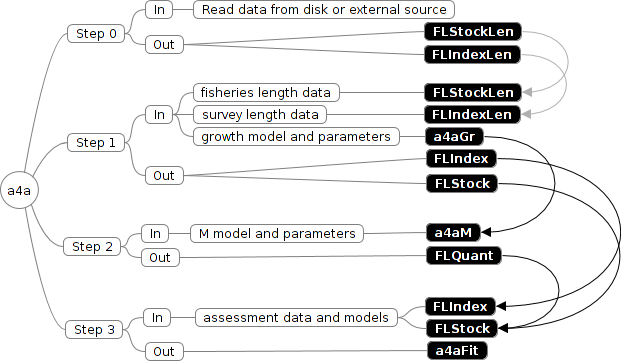
\includegraphics[width=\textwidth]{./inout}
\caption{In/out process of the \initiative{a4a} approach. The boxes in black represent the classes of the objects that carry the information in and out of each step.}
\label{fig:inout}
\end{figure}

Analysis related to projections and biological reference points are dealt with by the \pkg{FLR} packages \pkg{FLash} and \pkg{FLBRP}. As such the Initiative does not provide specific methods for these analyses.

In Steps 1 and 2 there is no fitting of growth models or natural mortality models. The rationale is to provide tools that allow the uncertainty associated with these processes to be carried on into the stock assessment, e.g. through parameter uncertainty. This approach allows the users to pick up the required information from other sources of information such as papers, PhDs, Fishbase, other stocks, etc. If the stock under analysis does not have specific information on the growth or natural mortality processes, generic information about life history invariants may be used such as the generic priors suggested by \href{http://icesjms.oxfordjournals.org/content/early/2014/03/04/icesjms.fsu023.abstract}{Bentley, (2014)}.

Note that an environment like the one distributed by \initiative{a4a} promotes the exploration of different models for each process, giving the analyst a lot of flexibility. It also opens the possibility to efficiently include distinct models in the analysis. For example, a stock assessment using two growth, or several models for natural mortality could be performed. Our suggestion to streamline the assessment process is to combine the final outcomes using model averaging (\href{http://icesjms.oxfordjournals.org/content/early/2014/03/31/icesjms.fsu043.abstract}{Miller, et. al, 2014}). Other solutions may be implemented, like scenario analysis, etc. What is important is to keep the data flowing smoothly and the models clear. R (\href{http://www.R-project.org/}{R Core Team, 2014}) and \pkg{FLR} (\href{http://icesjms.oxfordjournals.org/content/64/4/640.abstract}{Kell, et.al, 200}) provide powerful platforms for this approach.

\subsection{How to read this document}

The target audience for this document are readers with some experience in R and some background on stock assessment.

The document explains the approach being developed by \initiative{a4a} for fish stock assessment and scientific advice. It presents a mixture of text and code, where the first explains the concepts behind the methods, while the last shows how these can be run with the software provided. Moreover, having the code allows the reader to copy/paste and replicate the analysis presented here.

The sections and subsections are as independent as possible, so it can be used as a reference document for the \pkg{FLa4a}. 

Section~\ref{sec:in} deals with reading and preparing data in \pkg{FLR} objects, which constitute the basic dataset for stock assessment with length structured models. This section is independent from \pkg{FLa4a} and relies mostly on \R and \pkg{reshape}.

Sections~\ref{sec:l2a},\ref{sec:M} and \ref{sec:sca} are related with \pkg{FLa4a} and describe the concepts described in the previous section.

Finally, this document is a work in progress and will be updated and released often.

\subsubsection{Loading libraries, data and defining some useful functions}

To run the \pkg{FLa4a} methods the reader will need to install the package and its dependencies and load them, together with a couple of other packages. Some datsets are distributed with the package and as such need to be loaded too. A set of auxiliary functions are also required, to avoid having long and repetitive code.

\begin{knitrout}
\definecolor{shadecolor}{rgb}{0.949, 0.949, 0.949}\color{fgcolor}\begin{kframe}
\begin{alltt}
\hlcom{# from CRAN}
\hlkwd{install.packages}\hlstd{(}\hlkwd{c}\hlstd{(}\hlstr{"copula"}\hlstd{,}\hlstr{"triangle"}\hlstd{))}
\hlcom{# from FLR}
\hlkwd{install.packages}\hlstd{(}\hlkwd{c}\hlstd{(}\hlstr{"FLCore"}\hlstd{,} \hlstr{"FLa4a"}\hlstd{),} \hlkwc{repos}\hlstd{=}\hlstr{"http://flr-project.org/R"}\hlstd{)}
\end{alltt}
\end{kframe}
\end{knitrout}

\begin{knitrout}
\definecolor{shadecolor}{rgb}{0.949, 0.949, 0.949}\color{fgcolor}\begin{kframe}
\begin{alltt}
\hlcom{# libraries}
\hlkwd{library}\hlstd{(FLa4a)}
\hlkwd{library}\hlstd{(XML)}
\hlkwd{library}\hlstd{(reshape2)}
\hlkwd{library}\hlstd{(diagram)}
\hlkwd{library}\hlstd{(plot3D)}
\hlcom{# datasets}
\hlkwd{data}\hlstd{(ple4)}
\hlkwd{data}\hlstd{(ple4.indices)}
\hlkwd{data}\hlstd{(ple4.index)}
\hlkwd{data}\hlstd{(rfLen)}
\end{alltt}
\end{kframe}
\end{knitrout}

\begin{knitrout}
\definecolor{shadecolor}{rgb}{0.949, 0.949, 0.949}\color{fgcolor}\begin{kframe}
\begin{verbatim}
## [1] "wireframe"
## [1] "wireframe"
\end{verbatim}
\end{kframe}
\end{knitrout}

\begin{knitrout}
\definecolor{shadecolor}{rgb}{0.949, 0.949, 0.949}\color{fgcolor}\begin{kframe}
\begin{alltt}
\hlcom{# recode Gadget's length categories}
\hlstd{qt2qt} \hlkwb{<-} \hlkwa{function}\hlstd{(}\hlkwc{object}\hlstd{,} \hlkwc{id}\hlstd{=}\hlnum{5}\hlstd{,} \hlkwc{split}\hlstd{=}\hlstr{"-"}\hlstd{)\{}
        \hlstd{qt} \hlkwb{<-} \hlstd{object[,id]}
        \hlkwd{levels}\hlstd{(qt)} \hlkwb{<-} \hlkwd{unlist}\hlstd{(}\hlkwd{lapply}\hlstd{(}\hlkwd{strsplit}\hlstd{(}\hlkwd{levels}\hlstd{(qt),} \hlkwc{split}\hlstd{=split),} \hlstr{"[["}\hlstd{,} \hlnum{2}\hlstd{))}
        \hlkwd{as.numeric}\hlstd{(}\hlkwd{as.character}\hlstd{(qt))}
\hlstd{\}}

\hlcom{# function to check import and do some massage}
\hlstd{cim} \hlkwb{<-} \hlkwa{function}\hlstd{(}\hlkwc{object}\hlstd{,} \hlkwc{n}\hlstd{,} \hlkwc{wt}\hlstd{,} \hlkwc{hrv}\hlstd{=}\hlstr{"missing"}\hlstd{)\{}
        \hlstd{v} \hlkwb{<-} \hlstd{object[}\hlkwd{sample}\hlstd{(}\hlnum{1}\hlopt{:}\hlkwd{nrow}\hlstd{(object),} \hlnum{1}\hlstd{),]}
        \hlstd{c1} \hlkwb{<-} \hlkwd{c}\hlstd{(n[}\hlkwd{as.character}\hlstd{(v}\hlopt{$}\hlstd{V5),}\hlkwd{as.character}\hlstd{(v}\hlopt{$}\hlstd{V1),}\hlnum{1}\hlstd{,}\hlkwd{as.character}\hlstd{(v}\hlopt{$}\hlstd{V2)]}\hlopt{==}\hlstd{v}\hlopt{$}\hlstd{V6)}
        \hlstd{c2} \hlkwb{<-} \hlkwd{c}\hlstd{(wt[}\hlkwd{as.character}\hlstd{(v}\hlopt{$}\hlstd{V5),}\hlkwd{as.character}\hlstd{(v}\hlopt{$}\hlstd{V1),}\hlnum{1}\hlstd{,}\hlkwd{as.character}\hlstd{(v}\hlopt{$}\hlstd{V2)]}\hlopt{==}\hlstd{v}\hlopt{$}\hlstd{V7)}
        \hlkwa{if}\hlstd{(}\hlkwd{missing}\hlstd{(hrv))\{}
                \hlstd{c1} \hlopt{+} \hlstd{c2} \hlopt{==} \hlnum{2}
        \hlstd{\}} \hlkwa{else} \hlstd{\{}
                \hlstd{c3} \hlkwb{<-} \hlkwd{c}\hlstd{(hrv[}\hlkwd{as.character}\hlstd{(v}\hlopt{$}\hlstd{V5),}\hlkwd{as.character}\hlstd{(v}\hlopt{$}\hlstd{V1),}\hlnum{1}\hlstd{,}\hlkwd{as.character}\hlstd{(v}\hlopt{$}\hlstd{V2)]}\hlopt{==}\hlstd{v}\hlopt{$}\hlstd{V8)}
                \hlstd{c1} \hlopt{+} \hlstd{c2} \hlopt{+} \hlstd{c3} \hlopt{==} \hlnum{3}
        \hlstd{\}}
\hlstd{\}}

\hlcom{# plot for S4 data structures with diagram}
\hlstd{plotS4} \hlkwb{<-} \hlkwa{function}\hlstd{(}\hlkwc{object}\hlstd{,} \hlkwc{linktext}\hlstd{=}\hlstr{"typeof"}\hlstd{,} \hlkwc{main}\hlstd{=}\hlstr{"S4 class"}\hlstd{,} \hlkwc{...}\hlstd{)\{}
        \hlstd{args} \hlkwb{<-} \hlkwd{list}\hlstd{(...)}
        \hlstd{obj} \hlkwb{<-} \hlkwd{getClass}\hlstd{(}\hlkwd{as.character}\hlstd{(object))}
        \hlstd{df0} \hlkwb{<-} \hlkwd{data.frame}\hlstd{(}\hlkwd{names}\hlstd{(obj}\hlopt{@}\hlkwc{slots}\hlstd{),} \hlkwd{unlist}\hlstd{(}\hlkwd{lapply}\hlstd{(obj}\hlopt{@}\hlkwc{slots}\hlstd{,} \hlstr{"[["}\hlstd{,} \hlnum{1}\hlstd{)))}
        \hlstd{nms} \hlkwb{<-} \hlkwd{c}\hlstd{(}\hlkwd{t}\hlstd{(df0))}
        \hlstd{nslts} \hlkwb{<-} \hlkwd{length}\hlstd{(nms)}\hlopt{/}\hlnum{2}
        \hlstd{M} \hlkwb{<-} \hlkwd{matrix}\hlstd{(}\hlkwc{nrow} \hlstd{=} \hlkwd{length}\hlstd{(nms),} \hlkwc{ncol} \hlstd{=} \hlkwd{length}\hlstd{(nms),} \hlkwc{byrow} \hlstd{=} \hlnum{TRUE}\hlstd{,} \hlkwc{data} \hlstd{=} \hlnum{0}\hlstd{)}
        \hlkwa{for}\hlstd{(i} \hlkwa{in} \hlnum{1}\hlopt{:}\hlstd{nslts)\{}
                \hlstd{M[i}\hlopt{*}\hlnum{2}\hlstd{,i}\hlopt{*}\hlnum{2}\hlopt{-}\hlnum{1}\hlstd{]} \hlkwb{<-} \hlstd{linktext}
        \hlstd{\}}
        \hlstd{args}\hlopt{$}\hlstd{A}\hlkwb{=}\hlstd{M}
        \hlstd{args}\hlopt{$}\hlstd{pos}\hlkwb{=}\hlkwd{rep}\hlstd{(}\hlnum{2}\hlstd{,} \hlkwd{length}\hlstd{(nms)}\hlopt{/}\hlnum{2}\hlstd{)}
        \hlstd{args}\hlopt{$}\hlstd{name} \hlkwb{=} \hlstd{nms}
        \hlstd{args}\hlopt{$}\hlstd{main}\hlkwb{=}\hlstd{main}
        \hlkwd{do.call}\hlstd{(}\hlstr{"plotmat"}\hlstd{, args)}
\hlstd{\}}
\end{alltt}
\end{kframe}
\end{knitrout}

\section{Reading files and building \pkg{FLR} objects}\label{sec:in}

For this document we'll use the plaice in ICES area IV dataset, provided by \pkg{FLR}, and a length-based simulated dataset based on red fish, using \href{http://www.hafro.is/gadget}{\pkg{Gadget}}, provided by Daniel Howell (Institute of Marine Research, Norway). In this section we'll read in the \pkg{Gadget} data files, and transform them into \pkg{FLR} objects, by first reading the files as data frames, recode some variables and finally creating \pkg{FLR} objects. Note that the following code assumes that the files are in the working directory.

\begin{knitrout}
\definecolor{shadecolor}{rgb}{0.949, 0.949, 0.949}\color{fgcolor}\begin{kframe}
\begin{alltt}
\hlcom{# catch}
\hlstd{cth.orig} \hlkwb{<-} \hlkwd{read.table}\hlstd{(}\hlstr{"catch.len"}\hlstd{,} \hlkwc{skip}\hlstd{=}\hlnum{5}\hlstd{)}

\hlcom{# check the format of the files}
\hlkwd{head}\hlstd{(cth.orig)}
\end{alltt}
\begin{verbatim}
##     V1 V2       V3      V4          V5        V6        V7        V8
## 1 1986  1 allareas allages len-1.0-2.0 0.0001290 6.532e-09 3.796e-08
## 2 1986  1 allareas allages len-2.0-3.0 0.0004493 1.053e-07 6.102e-08
## 3 1986  1 allareas allages len-3.0-4.0 0.0014999 9.646e-07 9.807e-08
## 4 1986  1 allareas allages len-4.0-5.0 0.0047867 6.543e-06 1.576e-07
## 5 1986  1 allareas allages len-5.0-6.0 0.0145722 3.637e-05 2.533e-07
## 6 1986  1 allareas allages len-6.0-7.0 0.0422405 1.740e-04 4.072e-07
\end{verbatim}
\begin{alltt}
\hlcom{# stock}
\hlstd{stk.orig} \hlkwb{<-} \hlkwd{read.table}\hlstd{(}\hlstr{"red.len"}\hlstd{,} \hlkwc{skip}\hlstd{=}\hlnum{4}\hlstd{)}

\hlcom{# surveys}
\hlstd{idx.orig} \hlkwb{<-} \hlkwd{read.table}\hlstd{(}\hlstr{"survey.len"}\hlstd{,} \hlkwc{skip}\hlstd{=}\hlnum{5}\hlstd{)}
\hlstd{idxJmp.orig} \hlkwb{<-} \hlkwd{read.table}\hlstd{(}\hlstr{"jump.survey.len"}\hlstd{,} \hlkwc{skip}\hlstd{=}\hlnum{5}\hlstd{)}
\hlstd{idxTrd.orig} \hlkwb{<-} \hlkwd{read.table}\hlstd{(}\hlstr{"tend.survey.len"}\hlstd{,} \hlkwc{skip}\hlstd{=}\hlnum{5}\hlstd{)}

\hlcom{# Recode the length categories into something usable}

\hlcom{# catch}
\hlstd{cth.orig[,}\hlnum{5}\hlstd{]} \hlkwb{<-} \hlkwd{qt2qt}\hlstd{(cth.orig)}

\hlcom{# stock}
\hlstd{stk.orig[,}\hlnum{5}\hlstd{]} \hlkwb{<-} \hlkwd{qt2qt}\hlstd{(stk.orig)}

\hlcom{# surveys}
\hlstd{idx.orig[,}\hlnum{5}\hlstd{]} \hlkwb{<-} \hlkwd{qt2qt}\hlstd{(idx.orig)}
\hlstd{idxJmp.orig[,}\hlnum{5}\hlstd{]} \hlkwb{<-} \hlkwd{qt2qt}\hlstd{(idxJmp.orig)}
\hlstd{idxTrd.orig[,}\hlnum{5}\hlstd{]} \hlkwb{<-} \hlkwd{qt2qt}\hlstd{(idxTrd.orig)}
\end{alltt}
\end{kframe}
\end{knitrout}

Then we reshape the data frames into six dimensional arrays using \code{cast()} from package \pkg{reshape2}. Note that the columns names are \code{V\#} due to the importing method, which will have to be used in the formula argument to \code{acast}.

\begin{knitrout}
\definecolor{shadecolor}{rgb}{0.949, 0.949, 0.949}\color{fgcolor}\begin{kframe}
\begin{alltt}
\hlcom{# catch}
\hlstd{cth.n} \hlkwb{<-} \hlkwd{acast}\hlstd{(V5}\hlopt{~}\hlstd{V1}\hlopt{~}\hlnum{1}\hlopt{~}\hlstd{V2}\hlopt{~}\hlnum{1}\hlopt{~}\hlnum{1}\hlstd{,} \hlkwc{value.var}\hlstd{=}\hlstr{"V6"}\hlstd{,} \hlkwc{data}\hlstd{=cth.orig)}
\hlstd{cth.wt} \hlkwb{<-} \hlkwd{acast}\hlstd{(V5}\hlopt{~}\hlstd{V1}\hlopt{~}\hlnum{1}\hlopt{~}\hlstd{V2}\hlopt{~}\hlnum{1}\hlopt{~}\hlnum{1}\hlstd{,} \hlkwc{value.var}\hlstd{=}\hlstr{"V7"}\hlstd{,} \hlkwc{data}\hlstd{=cth.orig)}
\hlstd{hrv} \hlkwb{<-} \hlkwd{acast}\hlstd{(V5}\hlopt{~}\hlstd{V1}\hlopt{~}\hlnum{1}\hlopt{~}\hlstd{V2}\hlopt{~}\hlnum{1}\hlopt{~}\hlnum{1}\hlstd{,} \hlkwc{value.var}\hlstd{=}\hlstr{"V8"}\hlstd{,} \hlkwc{data}\hlstd{=cth.orig)}

\hlcom{# stock}
\hlstd{stk.n} \hlkwb{<-} \hlkwd{acast}\hlstd{(V5}\hlopt{~}\hlstd{V1}\hlopt{~}\hlnum{1}\hlopt{~}\hlstd{V2}\hlopt{~}\hlnum{1}\hlopt{~}\hlnum{1}\hlstd{,} \hlkwc{value.var}\hlstd{=}\hlstr{"V6"}\hlstd{,} \hlkwc{data}\hlstd{=stk.orig)}
\hlstd{stk.wt} \hlkwb{<-} \hlkwd{acast}\hlstd{(V5}\hlopt{~}\hlstd{V1}\hlopt{~}\hlnum{1}\hlopt{~}\hlstd{V2}\hlopt{~}\hlnum{1}\hlopt{~}\hlnum{1}\hlstd{,} \hlkwc{value.var}\hlstd{=}\hlstr{"V7"}\hlstd{,} \hlkwc{data}\hlstd{=stk.orig)}

\hlcom{# surveys}
\hlstd{idx.n} \hlkwb{<-} \hlkwd{acast}\hlstd{(V5}\hlopt{~}\hlstd{V1}\hlopt{~}\hlnum{1}\hlopt{~}\hlstd{V2}\hlopt{~}\hlnum{1}\hlopt{~}\hlnum{1}\hlstd{,} \hlkwc{value.var}\hlstd{=}\hlstr{"V6"}\hlstd{,} \hlkwc{data}\hlstd{=idx.orig)}
\hlstd{idx.wt} \hlkwb{<-} \hlkwd{acast}\hlstd{(V5}\hlopt{~}\hlstd{V1}\hlopt{~}\hlnum{1}\hlopt{~}\hlstd{V2}\hlopt{~}\hlnum{1}\hlopt{~}\hlnum{1}\hlstd{,} \hlkwc{value.var}\hlstd{=}\hlstr{"V7"}\hlstd{,} \hlkwc{data}\hlstd{=idx.orig)}
\hlstd{idx.hrv} \hlkwb{<-} \hlkwd{acast}\hlstd{(V5}\hlopt{~}\hlstd{V1}\hlopt{~}\hlnum{1}\hlopt{~}\hlstd{V2}\hlopt{~}\hlnum{1}\hlopt{~}\hlnum{1}\hlstd{,} \hlkwc{value.var}\hlstd{=}\hlstr{"V8"}\hlstd{,} \hlkwc{data}\hlstd{=idx.orig)}
\hlstd{idxJmp.n} \hlkwb{<-} \hlkwd{acast}\hlstd{(V5}\hlopt{~}\hlstd{V1}\hlopt{~}\hlnum{1}\hlopt{~}\hlstd{V2}\hlopt{~}\hlnum{1}\hlopt{~}\hlnum{1}\hlstd{,} \hlkwc{value.var}\hlstd{=}\hlstr{"V6"}\hlstd{,} \hlkwc{data}\hlstd{=idxJmp.orig)}
\hlstd{idxJmp.wt} \hlkwb{<-} \hlkwd{acast}\hlstd{(V5}\hlopt{~}\hlstd{V1}\hlopt{~}\hlnum{1}\hlopt{~}\hlstd{V2}\hlopt{~}\hlnum{1}\hlopt{~}\hlnum{1}\hlstd{,} \hlkwc{value.var}\hlstd{=}\hlstr{"V7"}\hlstd{,} \hlkwc{data}\hlstd{=idxJmp.orig)}
\hlstd{idxJmp.hrv} \hlkwb{<-} \hlkwd{acast}\hlstd{(V5}\hlopt{~}\hlstd{V1}\hlopt{~}\hlnum{1}\hlopt{~}\hlstd{V2}\hlopt{~}\hlnum{1}\hlopt{~}\hlnum{1}\hlstd{,} \hlkwc{value.var}\hlstd{=}\hlstr{"V8"}\hlstd{,} \hlkwc{data}\hlstd{=idxJmp.orig)}
\hlstd{idxTrd.n} \hlkwb{<-} \hlkwd{acast}\hlstd{(V5}\hlopt{~}\hlstd{V1}\hlopt{~}\hlnum{1}\hlopt{~}\hlstd{V2}\hlopt{~}\hlnum{1}\hlopt{~}\hlnum{1}\hlstd{,} \hlkwc{value.var}\hlstd{=}\hlstr{"V6"}\hlstd{,} \hlkwc{data}\hlstd{=idxTrd.orig)}
\hlstd{idxTrd.wt} \hlkwb{<-} \hlkwd{acast}\hlstd{(V5}\hlopt{~}\hlstd{V1}\hlopt{~}\hlnum{1}\hlopt{~}\hlstd{V2}\hlopt{~}\hlnum{1}\hlopt{~}\hlnum{1}\hlstd{,} \hlkwc{value.var}\hlstd{=}\hlstr{"V7"}\hlstd{,} \hlkwc{data}\hlstd{=idxTrd.orig)}
\hlstd{idxTrd.hrv} \hlkwb{<-} \hlkwd{acast}\hlstd{(V5}\hlopt{~}\hlstd{V1}\hlopt{~}\hlnum{1}\hlopt{~}\hlstd{V2}\hlopt{~}\hlnum{1}\hlopt{~}\hlnum{1}\hlstd{,} \hlkwc{value.var}\hlstd{=}\hlstr{"V8"}\hlstd{,} \hlkwc{data}\hlstd{=idxTrd.orig)}
\end{alltt}
\end{kframe}
\end{knitrout}

We take the arrays and make \class{FLQuant} objects from them.

\begin{knitrout}
\definecolor{shadecolor}{rgb}{0.949, 0.949, 0.949}\color{fgcolor}\begin{kframe}
\begin{alltt}
\hlcom{# catch}
\hlstd{dnms} \hlkwb{<-} \hlkwd{dimnames}\hlstd{(cth.n)}
\hlkwd{names}\hlstd{(dnms)} \hlkwb{<-} \hlkwd{names}\hlstd{(}\hlkwd{dimnames}\hlstd{(}\hlkwd{FLQuant}\hlstd{()))}
\hlkwd{names}\hlstd{(dnms)[}\hlnum{1}\hlstd{]} \hlkwb{<-} \hlstr{"len"}
\hlstd{cth.n} \hlkwb{<-} \hlkwd{FLQuant}\hlstd{(cth.n,} \hlkwc{dimnames}\hlstd{=dnms)}
\hlstd{cth.wt} \hlkwb{<-} \hlkwd{FLQuant}\hlstd{(cth.wt,} \hlkwc{dimnames}\hlstd{=dnms)}
\hlstd{hrv} \hlkwb{<-} \hlkwd{FLQuant}\hlstd{(hrv,} \hlkwc{dimnames}\hlstd{=dnms)}
\hlkwd{units}\hlstd{(hrv)} \hlkwb{<-} \hlstr{"f"}

\hlcom{# stock}
\hlstd{dnms} \hlkwb{<-} \hlkwd{dimnames}\hlstd{(stk.n)}
\hlkwd{names}\hlstd{(dnms)} \hlkwb{<-} \hlkwd{names}\hlstd{(}\hlkwd{dimnames}\hlstd{(}\hlkwd{FLQuant}\hlstd{()))}
\hlkwd{names}\hlstd{(dnms)[}\hlnum{1}\hlstd{]} \hlkwb{<-} \hlstr{"len"}
\hlstd{stk.n} \hlkwb{<-} \hlkwd{FLQuant}\hlstd{(stk.n,} \hlkwc{dimnames}\hlstd{=dnms)}
\hlstd{stk.wt} \hlkwb{<-} \hlkwd{FLQuant}\hlstd{(stk.wt,} \hlkwc{dimnames}\hlstd{=dnms)}

\hlcom{# surveys}
\hlstd{dnms} \hlkwb{<-} \hlkwd{dimnames}\hlstd{(idx.n)}
\hlkwd{names}\hlstd{(dnms)} \hlkwb{<-} \hlkwd{names}\hlstd{(}\hlkwd{dimnames}\hlstd{(}\hlkwd{FLQuant}\hlstd{()))}
\hlkwd{names}\hlstd{(dnms)[}\hlnum{1}\hlstd{]} \hlkwb{<-} \hlstr{"len"}
\hlstd{idx.n} \hlkwb{<-} \hlkwd{FLQuant}\hlstd{(idx.n,} \hlkwc{dimnames}\hlstd{=dnms)}
\hlstd{idx.wt} \hlkwb{<-} \hlkwd{FLQuant}\hlstd{(idx.wt,} \hlkwc{dimnames}\hlstd{=dnms)}
\hlstd{idx.hrv} \hlkwb{<-} \hlkwd{FLQuant}\hlstd{(idx.hrv,} \hlkwc{dimnames}\hlstd{=dnms)}

\hlstd{dnms} \hlkwb{<-} \hlkwd{dimnames}\hlstd{(idxJmp.n)}
\hlkwd{names}\hlstd{(dnms)} \hlkwb{<-} \hlkwd{names}\hlstd{(}\hlkwd{dimnames}\hlstd{(}\hlkwd{FLQuant}\hlstd{()))}
\hlkwd{names}\hlstd{(dnms)[}\hlnum{1}\hlstd{]} \hlkwb{<-} \hlstr{"len"}
\hlstd{idxJmp.n} \hlkwb{<-} \hlkwd{FLQuant}\hlstd{(idxJmp.n,} \hlkwc{dimnames}\hlstd{=dnms)}
\hlstd{idxJmp.wt} \hlkwb{<-} \hlkwd{FLQuant}\hlstd{(idxJmp.wt,} \hlkwc{dimnames}\hlstd{=dnms)}
\hlstd{idxJmp.hrv} \hlkwb{<-} \hlkwd{FLQuant}\hlstd{(idxJmp.hrv,} \hlkwc{dimnames}\hlstd{=dnms)}

\hlstd{dnms} \hlkwb{<-} \hlkwd{dimnames}\hlstd{(idxTrd.n)}
\hlkwd{names}\hlstd{(dnms)} \hlkwb{<-} \hlkwd{names}\hlstd{(}\hlkwd{dimnames}\hlstd{(}\hlkwd{FLQuant}\hlstd{()))}
\hlkwd{names}\hlstd{(dnms)[}\hlnum{1}\hlstd{]} \hlkwb{<-} \hlstr{"len"}
\hlstd{idxTrd.n} \hlkwb{<-} \hlkwd{FLQuant}\hlstd{(idxTrd.n,} \hlkwc{dimnames}\hlstd{=dnms)}
\hlstd{idxTrd.wt} \hlkwb{<-} \hlkwd{FLQuant}\hlstd{(idxTrd.wt,} \hlkwc{dimnames}\hlstd{=dnms)}
\hlstd{idxTrd.hrv} \hlkwb{<-} \hlkwd{FLQuant}\hlstd{(idxTrd.hrv,} \hlkwc{dimnames}\hlstd{=dnms)}
\end{alltt}
\end{kframe}
\end{knitrout}

Some sanity checks to check that the resulting objects have matching dimensions.

\begin{knitrout}
\definecolor{shadecolor}{rgb}{0.949, 0.949, 0.949}\color{fgcolor}\begin{kframe}
\begin{alltt}
\hlcom{# catch}
\hlkwd{cim}\hlstd{(cth.orig, cth.n, cth.wt, hrv)}
\end{alltt}
\begin{verbatim}
## [1] TRUE
\end{verbatim}
\begin{alltt}
\hlcom{# stock}
\hlkwd{cim}\hlstd{(stk.orig, stk.n, stk.wt)}
\end{alltt}
\begin{verbatim}
## [1] TRUE
\end{verbatim}
\begin{alltt}
\hlcom{# surveys}
\hlkwd{cim}\hlstd{(idx.orig, idx.n, idx.wt, idx.hrv)}
\end{alltt}
\begin{verbatim}
## [1] TRUE
\end{verbatim}
\begin{alltt}
\hlkwd{cim}\hlstd{(idxJmp.orig, idxJmp.n, idxJmp.wt, idxJmp.hrv)}
\end{alltt}
\begin{verbatim}
## [1] TRUE
\end{verbatim}
\begin{alltt}
\hlkwd{cim}\hlstd{(idxTrd.orig, idxTrd.n, idxTrd.wt, idxTrd.hrv)}
\end{alltt}
\begin{verbatim}
## [1] TRUE
\end{verbatim}
\end{kframe}
\end{knitrout}

Finally, we make \pkg{FLR} objects from the data.

\begin{knitrout}
\definecolor{shadecolor}{rgb}{0.949, 0.949, 0.949}\color{fgcolor}\begin{kframe}
\begin{alltt}
\hlcom{# stock}
\hlstd{rfLen.stk} \hlkwb{<-} \hlkwd{FLStockLen}\hlstd{(}\hlkwc{stock.n}\hlstd{=stk.n,} \hlkwc{stock.wt}\hlstd{=stk.wt,} \hlkwc{stock}\hlstd{=}\hlkwd{quantSums}\hlstd{(stk.wt}\hlopt{*}\hlstd{stk.n),} \hlkwc{catch.n}\hlstd{=cth.n,} \hlkwc{catch.wt}\hlstd{=cth.wt}\hlopt{/}\hlstd{cth.n,} \hlkwc{catch}\hlstd{=}\hlkwd{quantSums}\hlstd{(cth.wt),} \hlkwc{harvest}\hlstd{=hrv)}
\hlkwd{m}\hlstd{(rfLen.stk)[]} \hlkwb{<-} \hlnum{0.05}
\hlkwd{mat}\hlstd{(rfLen.stk)[]} \hlkwb{<-} \hlkwd{m.spwn}\hlstd{(rfLen.stk)[]} \hlkwb{<-} \hlkwd{harvest.spwn}\hlstd{(rfLen.stk)[]} \hlkwb{<-} \hlnum{0}
\hlkwd{mat}\hlstd{(rfLen.stk)[}\hlnum{38}\hlopt{:}\hlnum{59}\hlstd{,,,}\hlnum{3}\hlopt{:}\hlnum{4}\hlstd{]} \hlkwb{<-} \hlnum{1}

\hlcom{# surveys}
\hlstd{rfTrawl.idx} \hlkwb{<-} \hlkwd{FLIndex}\hlstd{(}\hlkwc{index}\hlstd{=idx.n,} \hlkwc{catch.n}\hlstd{=idx.n,} \hlkwc{catch.wt}\hlstd{=idx.wt,} \hlkwc{sel.pattern}\hlstd{=idx.hrv)}
\hlkwd{effort}\hlstd{(rfTrawl.idx)[]} \hlkwb{<-} \hlnum{100}

\hlstd{rfTrawlJmp.idx} \hlkwb{<-} \hlkwd{FLIndex}\hlstd{(}\hlkwc{index}\hlstd{=idxJmp.n,} \hlkwc{catch.n}\hlstd{=idxJmp.n,} \hlkwc{catch.wt}\hlstd{=idxJmp.wt,} \hlkwc{sel.pattern}\hlstd{=idxJmp.hrv)}
\hlkwd{effort}\hlstd{(rfTrawlJmp.idx)[]} \hlkwb{<-} \hlnum{100}

\hlstd{rfTrawlTrd.idx} \hlkwb{<-} \hlkwd{FLIndex}\hlstd{(}\hlkwc{index}\hlstd{=idxTrd.n,} \hlkwc{catch.n}\hlstd{=idxTrd.n,} \hlkwc{catch.wt}\hlstd{=idxTrd.wt,} \hlkwc{sel.pattern}\hlstd{=idxTrd.hrv)}
\hlkwd{effort}\hlstd{(rfTrawlTrd.idx)[]} \hlkwb{<-} \hlnum{100}
\end{alltt}
\end{kframe}
\end{knitrout}

\pagebreak
\section{Converting from length to age based data}\label{sec:l2a}

The \initiative{a4a} stock assessment framework is based on age dynamics. Therefore, to use length information it must be processed before it can be used in an assessment. The rationale is that the processing should give the analyst the flexibility to use a range of sources of information, \emph{e.g.} literature or online databases, to grab information about the species growth model and the uncertainty about the model parameters.

Within the \initiative{a4a} framework this is handled using the \class{a4aGr} class. In this section we introduce the \class{a4aGr} class and look at the variety of ways that parameter uncertainty can be included.

\subsection{a4aGr - The growth class}

The conversion of length data to age is performed through the use of a growth model. The implementation is done through the \class{a4aGr} class.

\begin{knitrout}
\definecolor{shadecolor}{rgb}{0.949, 0.949, 0.949}\color{fgcolor}\begin{kframe}
\begin{alltt}
\hlkwd{showClass}\hlstd{(}\hlstr{"a4aGr"}\hlstd{)}
\end{alltt}
\begin{verbatim}
## Class "a4aGr" [package "FLa4a"]
## 
## Slots:
##                                                                   
## Name:      grMod  grInvMod    params      vcov     distr      name
## Class:   formula   formula     FLPar     array character character
##                           
## Name:       desc     range
## Class: character   numeric
## 
## Extends: "FLComp"
\end{verbatim}
\end{kframe}
\end{knitrout}

To construct an \class{a4aGr} object, the growth model and parameters must be provided.
Check the help file for more information.

Here we show an example using the von Bertalanffy growth model. To create the \class{a4aGr} object it's necessary to pass the model equation ($length \sim time$), the inverse model equation ($time \sim length$) and the parameters. Any growth model can be used as long as it's possible to write the model (and the inverse) as an R formula.

\begin{knitrout}
\definecolor{shadecolor}{rgb}{0.949, 0.949, 0.949}\color{fgcolor}\begin{kframe}
\begin{alltt}
\hlstd{vbObj} \hlkwb{<-} \hlkwd{a4aGr}\hlstd{(}
        \hlkwc{grMod}\hlstd{=}\hlopt{~}\hlstd{linf}\hlopt{*}\hlstd{(}\hlnum{1}\hlopt{-}\hlkwd{exp}\hlstd{(}\hlopt{-}\hlstd{k}\hlopt{*}\hlstd{(t}\hlopt{-}\hlstd{t0))),}
        \hlkwc{grInvMod}\hlstd{=}\hlopt{~}\hlstd{t0}\hlopt{-}\hlnum{1}\hlopt{/}\hlstd{k}\hlopt{*}\hlkwd{log}\hlstd{(}\hlnum{1}\hlopt{-}\hlstd{len}\hlopt{/}\hlstd{linf),}
        \hlkwc{params}\hlstd{=}\hlkwd{FLPar}\hlstd{(}\hlkwc{linf}\hlstd{=}\hlnum{58.5}\hlstd{,} \hlkwc{k}\hlstd{=}\hlnum{0.086}\hlstd{,} \hlkwc{t0}\hlstd{=}\hlnum{0.001}\hlstd{,} \hlkwc{units}\hlstd{=}\hlkwd{c}\hlstd{(}\hlstr{"cm"}\hlstd{,}\hlstr{"ano-1"}\hlstd{,}\hlstr{"ano"}\hlstd{))}
\hlstd{)}

\hlcom{# Check the model and its inverse}
\hlstd{lc}\hlkwb{=}\hlnum{20}
\hlkwd{predict}\hlstd{(vbObj,} \hlkwc{len}\hlstd{=lc)}
\end{alltt}
\begin{verbatim}
##    iter
##         1
##   1 4.866
\end{verbatim}
\begin{alltt}
\hlkwd{predict}\hlstd{(vbObj,} \hlkwc{t}\hlstd{=}\hlkwd{predict}\hlstd{(vbObj,} \hlkwc{len}\hlstd{=lc))}\hlopt{==}\hlstd{lc}
\end{alltt}
\begin{verbatim}
##    iter
##        1
##   1 TRUE
\end{verbatim}
\end{kframe}
\end{knitrout}

The predict method allows the transformation between age and lengths using the growth model.

\begin{knitrout}
\definecolor{shadecolor}{rgb}{0.949, 0.949, 0.949}\color{fgcolor}\begin{kframe}
\begin{alltt}
\hlkwd{predict}\hlstd{(vbObj,} \hlkwc{len}\hlstd{=}\hlnum{5}\hlopt{:}\hlnum{10}\hlopt{+}\hlnum{0.5}\hlstd{)}
\end{alltt}
\begin{verbatim}
##    iter
##         1
##   1 1.149
##   2 1.371
##   3 1.596
##   4 1.827
##   5 2.062
##   6 2.301
\end{verbatim}
\begin{alltt}
\hlkwd{predict}\hlstd{(vbObj,} \hlkwc{t}\hlstd{=}\hlnum{5}\hlopt{:}\hlnum{10}\hlopt{+}\hlnum{0.5}\hlstd{)}
\end{alltt}
\begin{verbatim}
##    iter
##         1
##   1 22.04
##   2 25.05
##   3 27.80
##   4 30.33
##   5 32.66
##   6 34.78
\end{verbatim}
\end{kframe}
\end{knitrout}

\subsection{Adding uncertainty to growth parameters with a multivariate normal distribution}

Uncertainty in the growth model is introduced through the inclusion of parameter uncertainty.
This is done by making use of the parameter variance-covariance matrix (the \code{vcov} slot of the \class{a4aGr} class) and assuming a distribution. The numbers in the variance-covariance matrix could come from the parameter uncertainty from fitting the growth model parameters.

Here we set the variance-covariance matrix by scaling a correlation matrix, using a cv of 0.2.

\begin{knitrout}
\definecolor{shadecolor}{rgb}{0.949, 0.949, 0.949}\color{fgcolor}\begin{kframe}
\begin{alltt}
\hlcom{# Make an empty cor matrix}
\hlstd{cm} \hlkwb{<-} \hlkwd{diag}\hlstd{(}\hlkwd{c}\hlstd{(}\hlnum{1}\hlstd{,}\hlnum{1}\hlstd{,}\hlnum{1}\hlstd{))}
\hlcom{# k and linf are negatively correlated while t0 is independent}
\hlstd{cm[}\hlnum{1}\hlstd{,}\hlnum{2}\hlstd{]} \hlkwb{<-} \hlstd{cm[}\hlnum{2}\hlstd{,}\hlnum{1}\hlstd{]} \hlkwb{<-} \hlopt{-}\hlnum{0.5}
\hlcom{# scale cor to var using CV=0.2}
\hlstd{cv} \hlkwb{<-} \hlnum{0.2}
\hlstd{p} \hlkwb{<-} \hlkwd{c}\hlstd{(}\hlkwc{linf}\hlstd{=}\hlnum{60}\hlstd{,} \hlkwc{k}\hlstd{=}\hlnum{0.09}\hlstd{,} \hlkwc{t0}\hlstd{=}\hlopt{-}\hlnum{0.01}\hlstd{)}
\hlstd{vc} \hlkwb{<-} \hlkwd{matrix}\hlstd{(}\hlnum{1}\hlstd{,} \hlkwc{ncol}\hlstd{=}\hlnum{3}\hlstd{,} \hlkwc{nrow}\hlstd{=}\hlnum{3}\hlstd{)}
\hlstd{l} \hlkwb{<-} \hlstd{vc}
\hlstd{l[}\hlnum{1}\hlstd{,]} \hlkwb{<-} \hlstd{l[,}\hlnum{1}\hlstd{]} \hlkwb{<-} \hlstd{p[}\hlnum{1}\hlstd{]}\hlopt{*}\hlstd{cv}
\hlstd{k} \hlkwb{<-} \hlstd{vc}
\hlstd{k[,}\hlnum{2}\hlstd{]} \hlkwb{<-} \hlstd{k[}\hlnum{2}\hlstd{,]} \hlkwb{<-} \hlstd{p[}\hlnum{2}\hlstd{]}\hlopt{*}\hlstd{cv}
\hlstd{t} \hlkwb{<-} \hlstd{vc}
\hlstd{t[}\hlnum{3}\hlstd{,]} \hlkwb{<-} \hlstd{t[,}\hlnum{3}\hlstd{]} \hlkwb{<-} \hlstd{p[}\hlnum{3}\hlstd{]}\hlopt{*}\hlstd{cv}
\hlstd{mm} \hlkwb{<-} \hlstd{t}\hlopt{*}\hlstd{k}\hlopt{*}\hlstd{l}
\hlkwd{diag}\hlstd{(mm)} \hlkwb{<-} \hlkwd{diag}\hlstd{(mm)}\hlopt{^}\hlnum{2}
\hlstd{mm} \hlkwb{<-} \hlstd{mm}\hlopt{*}\hlstd{cm}
\hlcom{# check that we have the intended correlation}
\hlkwd{all.equal}\hlstd{(cm,} \hlkwd{cov2cor}\hlstd{(mm))}
\end{alltt}
\begin{verbatim}
## [1] TRUE
\end{verbatim}
\end{kframe}
\end{knitrout}

Create the a4aGr object as before but now we also include the vcov argument for the variance-covariance matrix.
\begin{knitrout}
\definecolor{shadecolor}{rgb}{0.949, 0.949, 0.949}\color{fgcolor}\begin{kframe}
\begin{alltt}
\hlstd{vbObj} \hlkwb{<-} \hlkwd{a4aGr}\hlstd{(}\hlkwc{grMod}\hlstd{=}\hlopt{~}\hlstd{linf}\hlopt{*}\hlstd{(}\hlnum{1}\hlopt{-}\hlkwd{exp}\hlstd{(}\hlopt{-}\hlstd{k}\hlopt{*}\hlstd{(t}\hlopt{-}\hlstd{t0))),} \hlkwc{grInvMod}\hlstd{=}\hlopt{~}\hlstd{t0}\hlopt{-}\hlnum{1}\hlopt{/}\hlstd{k}\hlopt{*}\hlkwd{log}\hlstd{(}\hlnum{1}\hlopt{-}\hlstd{len}\hlopt{/}\hlstd{linf),} \hlkwc{params}\hlstd{=}\hlkwd{FLPar}\hlstd{(}\hlkwc{linf}\hlstd{=p[}\hlstr{"linf"}\hlstd{],} \hlkwc{k}\hlstd{=p[}\hlstr{"k"}\hlstd{],} \hlkwc{t0}\hlstd{=p[}\hlstr{"t0"}\hlstd{],} \hlkwc{units}\hlstd{=}\hlkwd{c}\hlstd{(}\hlstr{"cm"}\hlstd{,}\hlstr{"ano-1"}\hlstd{,}\hlstr{"ano"}\hlstd{)),} \hlkwc{vcov}\hlstd{=mm)}
\end{alltt}
\end{kframe}
\end{knitrout}

First we show a simple example where we assume that the parameters are represented using a multivariate normal distribution.
% This covariance matrix can have iterations (i.e. each iteration can have a different covariance matrix). CHECK
% If the parameters or the covariance matrix have iterations then the medians accross iterations are computed before simulating. Check help for \code{mvrnorm} for more information.

\begin{knitrout}
\definecolor{shadecolor}{rgb}{0.949, 0.949, 0.949}\color{fgcolor}\begin{kframe}
\begin{alltt}
\hlcom{# Note that the object we have just created has a single iteration of each parameter}
\hlstd{vbObj}\hlopt{@}\hlkwc{params}
\end{alltt}
\begin{verbatim}
## An object of class "FLPar"
## params
##  linf     k    t0 
## 60.00  0.09 -0.01 
## units:  cm ano-1 ano
\end{verbatim}
\begin{alltt}
\hlkwd{dim}\hlstd{(vbObj}\hlopt{@}\hlkwc{params}\hlstd{)}
\end{alltt}
\begin{verbatim}
## [1] 3 1
\end{verbatim}
\begin{alltt}
\hlcom{# We simulate 10000 iterations from the a4aGr object by calling mvrnorm() using the the variance-covariance matrix we created earlier.}
\hlstd{vbNorm} \hlkwb{<-} \hlkwd{mvrnorm}\hlstd{(}\hlnum{10000}\hlstd{,vbObj)}
\hlcom{# Now we have 10000 iterations of each parameter, randomly sampled from the multivariate normal distribution}
\hlstd{vbNorm}\hlopt{@}\hlkwc{params}
\end{alltt}
\begin{verbatim}
## An object of class "FLPar"
## iters:  10000 
## 
## params
##                linf                   k                  t0 
## 59.8599263(12.1486)  0.0903261( 0.0183) -0.0099746( 0.0020) 
## units:  cm ano-1 ano
\end{verbatim}
\begin{alltt}
\hlkwd{dim}\hlstd{(vbNorm}\hlopt{@}\hlkwc{params}\hlstd{)}
\end{alltt}
\begin{verbatim}
## [1]     3 10000
\end{verbatim}
\end{kframe}
\end{knitrout}

We can now convert from length to ages data based on the 10000 parameter iterations. This gives us 10000 sets of age data. For example, here we convert a single length vector using each of the 10000 parameter iterations: 

\begin{knitrout}
\definecolor{shadecolor}{rgb}{0.949, 0.949, 0.949}\color{fgcolor}\begin{kframe}
\begin{alltt}
\hlstd{ages} \hlkwb{<-} \hlkwd{predict}\hlstd{(vbNorm,} \hlkwc{len}\hlstd{=}\hlnum{5}\hlopt{:}\hlnum{10}\hlopt{+}\hlnum{0.5}\hlstd{)}
\hlkwd{dim}\hlstd{(ages)}
\end{alltt}
\begin{verbatim}
## [1]     6 10000
\end{verbatim}
\begin{alltt}
\hlcom{# We show the first ten iterations only as an illustration}
\hlstd{ages[,}\hlnum{1}\hlopt{:}\hlnum{10}\hlstd{]}
\end{alltt}
\begin{verbatim}
##    iter
##         1     2     3     4     5      6     7     8     9    10
##   1 1.183 1.248 1.089 1.542 1.044 0.9086 0.893 1.252 1.281 1.169
##   2 1.413 1.486 1.298 1.840 1.243 1.0864 1.066 1.500 1.524 1.397
##   3 1.647 1.727 1.511 2.145 1.445 1.2678 1.241 1.754 1.771 1.629
##   4 1.885 1.971 1.727 2.455 1.648 1.4530 1.419 2.015 2.020 1.866
##   5 2.128 2.218 1.946 2.771 1.854 1.6422 1.601 2.283 2.272 2.109
##   6 2.376 2.467 2.169 3.093 2.063 1.8356 1.785 2.559 2.527 2.357
\end{verbatim}
\end{kframe}
\end{knitrout}

The marginal distributions can be seen in Figure~\ref{fig:plot_norm_params}.

\begin{knitrout}
\definecolor{shadecolor}{rgb}{0.949, 0.949, 0.949}\color{fgcolor}\begin{kframe}
\begin{alltt}
\hlkwd{par}\hlstd{(}\hlkwc{mfrow}\hlstd{=}\hlkwd{c}\hlstd{(}\hlnum{3}\hlstd{,}\hlnum{1}\hlstd{))}
\hlkwd{hist}\hlstd{(}\hlkwd{c}\hlstd{(}\hlkwd{params}\hlstd{(vbNorm)[}\hlstr{"linf"}\hlstd{,]),} \hlkwc{main}\hlstd{=}\hlstr{"linf"}\hlstd{,} \hlkwc{xlab}\hlstd{=}\hlstr{""}\hlstd{)}
\hlkwd{hist}\hlstd{(}\hlkwd{c}\hlstd{(}\hlkwd{params}\hlstd{(vbNorm)[}\hlstr{"k"}\hlstd{,]),} \hlkwc{main}\hlstd{=}\hlstr{"k"}\hlstd{,} \hlkwc{prob}\hlstd{=}\hlnum{TRUE}\hlstd{,} \hlkwc{xlab}\hlstd{=}\hlstr{""}\hlstd{)}
\hlkwd{hist}\hlstd{(}\hlkwd{c}\hlstd{(}\hlkwd{params}\hlstd{(vbNorm)[}\hlstr{"t0"}\hlstd{,]),} \hlkwc{main}\hlstd{=}\hlstr{"t0"}\hlstd{,} \hlkwc{xlab}\hlstd{=}\hlstr{""}\hlstd{)}
\end{alltt}
\end{kframe}\begin{figure}[H]


{\centering \includegraphics[width=\maxwidth]{figure/plot_norm_params} 

}

\caption[The marginal distributions of each of the parameters from using a multivariate normal distribution]{The marginal distributions of each of the parameters from using a multivariate normal distribution.\label{fig:plot_norm_params}}
\end{figure}


\end{knitrout}

The shape of the correlation can be seen in Figure~\ref{fig:plot_norm_scatter}.
\begin{knitrout}
\definecolor{shadecolor}{rgb}{0.949, 0.949, 0.949}\color{fgcolor}\begin{kframe}
\begin{alltt}
\hlkwd{splom}\hlstd{(}\hlkwd{data.frame}\hlstd{(}\hlkwd{t}\hlstd{(}\hlkwd{params}\hlstd{(vbNorm)}\hlopt{@}\hlkwc{.Data}\hlstd{)),} \hlkwc{pch}\hlstd{=}\hlstr{"."}\hlstd{)}
\end{alltt}
\end{kframe}\begin{figure}[H]


{\centering \includegraphics[width=\maxwidth]{figure/plot_norm_scatter} 

}

\caption[Scatter plot of the 10000 samples parameter from the multivariate normal distribution]{Scatter plot of the 10000 samples parameter from the multivariate normal distribution.\label{fig:plot_norm_scatter}}
\end{figure}


\end{knitrout}

Growth curves for the 1000 iterations can be seen in Figure~\ref{fig:plot_mv_growth}.

\begin{knitrout}
\definecolor{shadecolor}{rgb}{0.949, 0.949, 0.949}\color{fgcolor}\begin{kframe}
\begin{alltt}
\hlkwd{boxplot}\hlstd{(}\hlkwd{t}\hlstd{(}\hlkwd{predict}\hlstd{(vbNorm,} \hlkwc{t}\hlstd{=}\hlnum{0}\hlopt{:}\hlnum{50}\hlopt{+}\hlnum{0.5}\hlstd{)))}
\end{alltt}
\end{kframe}\begin{figure}[H]


{\centering \includegraphics[width=\maxwidth]{figure/plot_mv_growth} 

}

\caption[Growth curves using parameters simulated from a multivariate normal distribution]{Growth curves using parameters simulated from a multivariate normal distribution.\label{fig:plot_mv_growth}}
\end{figure}


\end{knitrout}

\subsection{Adding uncertainty to growth parameters with a multivariate triangle distribution}
\label{sec:growth_triangle_cop}

One alternative to using a normal distribution is to use a \href{http://en.wikipedia.org/wiki/Triangle\_distribution}{triangle distribution}. We use the package \href{http://cran.r-project.org/web/packages/triangle/index.html}{\pkg{triangle}}, where this distribution is parametrized using the minimum, maximum and median values. This can be very attractive if the analyst needs to scrape information from the web or literature and perform some kind of meta-analysis.

Here we show an example of setting a triangle distribution with values taken from Fishbase.

\begin{knitrout}
\definecolor{shadecolor}{rgb}{0.949, 0.949, 0.949}\color{fgcolor}\begin{kframe}
\begin{alltt}
\hlcom{# The web address for the growth parameters for redfish (Sebastes norvegicus)}
\hlstd{addr} \hlkwb{<-} \hlstr{"http://www.fishbase.org/PopDyn/PopGrowthList.php?ID=501"}
\hlcom{# Scrape the data}
\hlstd{tab} \hlkwb{<-} \hlkwd{try}\hlstd{(}\hlkwd{readHTMLTable}\hlstd{(addr))}
\hlcom{# Interrogate the data table and get vectors of the values}
\hlstd{linf} \hlkwb{<-} \hlkwd{as.numeric}\hlstd{(}\hlkwd{as.character}\hlstd{(tab}\hlopt{$}\hlstd{dataTable[,}\hlnum{2}\hlstd{]))}
\hlstd{k} \hlkwb{<-} \hlkwd{as.numeric}\hlstd{(}\hlkwd{as.character}\hlstd{(tab}\hlopt{$}\hlstd{dataTable[,}\hlnum{4}\hlstd{]))}
\hlstd{t0} \hlkwb{<-} \hlkwd{as.numeric}\hlstd{(}\hlkwd{as.character}\hlstd{(tab}\hlopt{$}\hlstd{dataTable[,}\hlnum{5}\hlstd{]))}
\hlcom{# Set the min (a), max (b) and median (c) values for the parameter as a list of lists}
\hlcom{# Note that t0 has no 'c' (median) value. This makes the distribution symmetrical}
\hlstd{triPars} \hlkwb{<-} \hlkwd{list}\hlstd{(}\hlkwd{list}\hlstd{(}\hlkwc{a}\hlstd{=}\hlkwd{min}\hlstd{(linf),} \hlkwc{b}\hlstd{=}\hlkwd{max}\hlstd{(linf),} \hlkwc{c}\hlstd{=}\hlkwd{median}\hlstd{(linf)),}
             \hlkwd{list}\hlstd{(}\hlkwc{a}\hlstd{=}\hlkwd{min}\hlstd{(k),} \hlkwc{b}\hlstd{=}\hlkwd{max}\hlstd{(k),} \hlkwc{c}\hlstd{=}\hlkwd{median}\hlstd{(k)),}
             \hlkwd{list}\hlstd{(}\hlkwc{a}\hlstd{=}\hlkwd{median}\hlstd{(t0,} \hlkwc{na.rm}\hlstd{=T)}\hlopt{-}\hlkwd{IQR}\hlstd{(t0,} \hlkwc{na.rm}\hlstd{=T)}\hlopt{/}\hlnum{2}\hlstd{,} \hlkwc{b}\hlstd{=}\hlkwd{median}\hlstd{(t0,} \hlkwc{na.rm}\hlstd{=T)}\hlopt{+}\hlkwd{IQR}\hlstd{(t0,} \hlkwc{na.rm}\hlstd{=T)}\hlopt{/}\hlnum{2}\hlstd{))}
\hlcom{# Simulate 10000 times using mvrtriangle}
\hlstd{vbTri} \hlkwb{<-} \hlkwd{mvrtriangle}\hlstd{(}\hlnum{10000}\hlstd{, vbObj,} \hlkwc{paramMargins}\hlstd{=triPars)}
\end{alltt}
\end{kframe}
\end{knitrout}

The marginals will reflect the uncertainty on the parameter values that were scraped from \href{http://fishbase.org}{Fishbase} but, as we don't really believe the parameters are multivariate normal, here we adopted a distribution based on a \emph{t} copula with triangle marginals.
The marginal distributions can be seen in Figure~\ref{fig:plot_tri_params} and the shape of the correlation can be seen in Figure~\ref{fig:plot_tri_scatter}.

\begin{knitrout}
\definecolor{shadecolor}{rgb}{0.949, 0.949, 0.949}\color{fgcolor}\begin{kframe}


{\ttfamily\noindent\bfseries\color{errorcolor}{\#\# Error: invalid number of 'breaks'}}

{\ttfamily\noindent\bfseries\color{errorcolor}{\#\# Error: invalid number of 'breaks'}}

{\ttfamily\noindent\bfseries\color{errorcolor}{\#\# Error: invalid number of 'breaks'}}\end{kframe}
\end{knitrout}

\begin{knitrout}
\definecolor{shadecolor}{rgb}{0.949, 0.949, 0.949}\color{fgcolor}\begin{kframe}


{\ttfamily\noindent\bfseries\color{errorcolor}{\#\# Error: Viewport 'plot\_01.panel.1.1.off.vp' was not found}}\end{kframe}\begin{figure}[H]


{\centering \includegraphics[width=\maxwidth]{figure/plot_tri_scatter} 

}

\caption[Scatter plot of the 10000 samples parameter from the multivariate triangle distribution]{Scatter plot of the 10000 samples parameter from the multivariate triangle distribution.\label{fig:plot_tri_scatter}}
\end{figure}


\end{knitrout}

We can still use \code{predict()} to see the growth model uncertainty (Figure~\ref{fig:plot_tri_growth}).

\begin{knitrout}
\definecolor{shadecolor}{rgb}{0.949, 0.949, 0.949}\color{fgcolor}\begin{kframe}


{\ttfamily\noindent\bfseries\color{errorcolor}{\#\# Error: need finite 'ylim' values}}\end{kframe}\begin{figure}[H]


{\centering \includegraphics[width=\maxwidth]{figure/plot_tri_growth} 

}

\caption[Growth curves using parameters simulated from a multivariate triangle distribution]{Growth curves using parameters simulated from a multivariate triangle distribution.\label{fig:plot_tri_growth}}
\end{figure}


\end{knitrout}

Remember that the above examples use a variance-covariance matrix that we essentially made up. An alternative would be to scrape the entire growth parameters dataset from Fishbase and compute the shape of the variance-covariance matrix yourself.

\subsection{Adding uncertainty to growth parameters with statistical copulas}

A more general approach to adding parameter uncertainty is to make use of \href{http://www.encyclopediaofmath.org/index.php/Copula}{statistical copulas} and marginal distributions of choice. This is possible with the \code{mvrcop()} function borrowed from the package \href{http://cran.r-project.org/web/packages/copula/}{\pkg{copula}}. The example below keeps the same parameters and changes only the copula type and family but a lot more can be done. Check the package \pkg{copula} for more information. 

% Needs more explanation

\begin{knitrout}
\definecolor{shadecolor}{rgb}{0.949, 0.949, 0.949}\color{fgcolor}\begin{kframe}
\begin{alltt}
\hlstd{vbCop} \hlkwb{<-} \hlkwd{mvrcop}\hlstd{(}\hlnum{10000}\hlstd{, vbObj,} \hlkwc{copula}\hlstd{=}\hlstr{"archmCopula"}\hlstd{,} \hlkwc{family}\hlstd{=}\hlstr{"clayton"}\hlstd{,} \hlkwc{param}\hlstd{=}\hlnum{2}\hlstd{,} \hlkwc{margins}\hlstd{=}\hlstr{"triangle"}\hlstd{,} \hlkwc{paramMargins}\hlstd{=triPars)}
\end{alltt}
\end{kframe}
\end{knitrout}

The shape of the correlation changes (Figure~\ref{fig:plot_cop_tri_scatter}) as well as the resulting growth curves (Figure~\ref{fig:plot_cop_tri_growth}). 

\begin{knitrout}
\definecolor{shadecolor}{rgb}{0.949, 0.949, 0.949}\color{fgcolor}\begin{kframe}


{\ttfamily\noindent\bfseries\color{errorcolor}{\#\# Error: Viewport 'plot\_01.panel.1.1.off.vp' was not found}}\end{kframe}\begin{figure}[H]


{\centering \includegraphics[width=\maxwidth]{figure/plot_cop_tri_scatter} 

}

\caption[Scatter plot of the 10000 samples parameter from the using an archmCopula copula with triangle margins]{Scatter plot of the 10000 samples parameter from the using an archmCopula copula with triangle margins.\label{fig:plot_cop_tri_scatter}}
\end{figure}


\end{knitrout}

\begin{knitrout}
\definecolor{shadecolor}{rgb}{0.949, 0.949, 0.949}\color{fgcolor}\begin{kframe}


{\ttfamily\noindent\bfseries\color{errorcolor}{\#\# Error: need finite 'ylim' values}}\end{kframe}\begin{figure}[H]


{\centering \includegraphics[width=\maxwidth]{figure/plot_cop_tri_growth} 

}

\caption[Growth curves from the using an archmCopula copula with triangle margins]{Growth curves from the using an archmCopula copula with triangle margins.\label{fig:plot_cop_tri_growth}}
\end{figure}


\end{knitrout}

\subsection{Converting from length to age based data - the \code{l2a()} method}

After introducing uncertainty in the growth model through the parameters it's time to transform the length-based dataset into an age-based dataset. The method that deals with this process is \code{l2a()}. The implementation of this method for the \class{FLQuant} class is the main workhorse. There are two other implementations, for the \class{FLStock} and \class{FLIndex} classes, which are mainly wrappers that call the \class{FLQuant} method several times.

When converting from length-based data to age-based data you need to be aware of how the aggregation of length classes is performed. For example, individuals in length classes 1-2, 2-3, and 3-4 cm may all be considered as being of age 1 (obviously depending on the growth model). How should the values in those length classes be combined?

If the values are abundances then the values should be summed. Summing other types of values, such as mean weight, does not make sense. Instead these values are averaged over the length classes (possibly weighted by the abundance). This is controlled using the \code{stat} argument which can be either \code{mean} or \code{sum} (the default). Fishing mortality is not computed to avoid making wrong assumptions about the meaning of F at length.

We demonstrate the method by converting a catch-at-length \class{FLQuant} to a catch-at-age \class{FLQuant}. First we make an \class{a4aGr} object with a multivariate triangle distribution (using the parameters we set above). We use 10 iterations as an example. And call \code{l2a()} by passing in the length-based \class{FLQuant} and the \class{a4aGr} object.

\begin{knitrout}
\definecolor{shadecolor}{rgb}{0.949, 0.949, 0.949}\color{fgcolor}\begin{kframe}
\begin{alltt}
\hlstd{vbTriSmall} \hlkwb{<-} \hlkwd{mvrtriangle}\hlstd{(}\hlnum{10}\hlstd{, vbObj,} \hlkwc{paramMargins}\hlstd{=triPars)}
\hlstd{cth.n} \hlkwb{<-} \hlkwd{l2a}\hlstd{(}\hlkwd{catch.n}\hlstd{(rfLen.stk), vbTriSmall)}
\end{alltt}


{\ttfamily\noindent\bfseries\color{errorcolor}{\#\# Error: argument of length 0}}\end{kframe}
\end{knitrout}

\begin{knitrout}
\definecolor{shadecolor}{rgb}{0.949, 0.949, 0.949}\color{fgcolor}\begin{kframe}
\begin{alltt}
\hlkwd{dim}\hlstd{(cth.n)}
\end{alltt}
\begin{verbatim}
## [1] 59 26  1  4  1  1
\end{verbatim}
\end{kframe}
\end{knitrout}

In the previous example, the \class{FLQuant} object that was sliced (\code{catch.n(rfLen.stk)}) had only one iteration. This iteration was sliced by each of the iterations in the growth model. It is possible for the \class{FLQuant} object to have the same number of iterations as the growth model, in which case each iteration of the \class{FLQuant} and the growth model are used together. It is also possible for the growth model to have only one iteration while the \class{FLQuant} object has many iterations. The same growth model is then used for each of the \class{FLQuant} iterations. As with all \pkg{FLR} objects, the general rule is \emph{one or n} iterations.


As well as converting one \class{FLQuant} at a time, we can convert entire \class{FLStock} and \class{FLIndex} objects. In these cases the individual \class{FLQuant} slots of those classes are converted from length-based to age-based. As mentioned above, the aggregation method depends on the type of values the slots contain. The abundance slots (\code{*.n}, such as \code{stock.n}) are summed. The \code{*.wt}, \code{m}, \code{mat}, \code{harvest.spwn} and \code{m.spwn} slots of an \class{FLStock} object are averaged. The \code{index}, \code{catch.wt}, \code{index.var}, \code{sel.pattern} and \code{index.q} slots of an \class{FLIndex} object are averaged.

The method for \class{FLStock} classes takes an additional argument for the plusgroup.

\begin{knitrout}
\definecolor{shadecolor}{rgb}{0.949, 0.949, 0.949}\color{fgcolor}\begin{kframe}
\begin{alltt}
\hlstd{aStk} \hlkwb{<-} \hlkwd{l2a}\hlstd{(rfLen.stk, vbTriSmall,} \hlkwc{plusgroup}\hlstd{=}\hlnum{14}\hlstd{)}
\end{alltt}


{\ttfamily\noindent\bfseries\color{errorcolor}{\#\# Error: argument of length 0}}\begin{alltt}
\hlstd{aIdx} \hlkwb{<-} \hlkwd{l2a}\hlstd{(rfTrawl.idx, vbTriSmall)}
\end{alltt}


{\ttfamily\noindent\bfseries\color{errorcolor}{\#\# Error: argument of length 0}}\end{kframe}
\end{knitrout}

When converting with \code{l2a()} all lengths above Linf are converted to the maximum age, as there is no information in the growth model about how to deal with individuals larger than Linf. 

\pagebreak
\section{Natural mortality}\label{sec:M}

In the \initiative{a4a} natural mortality is dealt with as an external parameter to the stock assessment model. The rationale to modelling natural mortality is similar to that of growth: one should be able to grab information from a range of sources and feed it into the assessment.

The mechanism used by \initiative{a4a} is to build an interface that makes it transparent, flexible and hopefully easy to explore different options. In relation to natural mortality it means that the analyst should be able to use distinct models like Gislasson's, Charnov's, Pauly's, etc in a coherent framework making it possible to compare the outcomes of the assessment. 

Within the \initiative{a4a} framework, the general method for inserting natural mortality in the stock assessment is to:

\begin{itemize}
    \item Create an object of class \class{a4aM} which holds the natural mortality model and parameters.
    \item Add uncertainty to the parameters in the \class{a4aM} object.
    \item Apply the \code{m()} method to the \class{a4aM} object to create an age or length based \class{FLQuant} object of the required dimensions.
\end{itemize}

The resulting \class{FLQuant} object can then be directly inserted into an \class {FLStock} object to be used for the assessment.   

In this section we go through each of the steps in detail using a variety of different models.

\subsection{\code{a4aM} - The M class}

Natural mortality is implemented in a class named \class{a4aM}. This class is made up of three objects of the class \class{FLModelSim}. Each object is a model that represents one effect: an age or length effect, a scaling (level) effect and a time trend, named \code{shape}, \code{level} and \code{trend}, respectively. The impact of the models is multiplicative, i.e. the overal natural mortality is given by \class{shape} x  \class{level} x \class{trend}. Check the help files for more information.

\begin{knitrout}
\definecolor{shadecolor}{rgb}{0.949, 0.949, 0.949}\color{fgcolor}\begin{kframe}
\begin{alltt}
\hlkwd{showClass}\hlstd{(}\hlstr{"a4aM"}\hlstd{)}
\end{alltt}
\begin{verbatim}
## Class "a4aM" [package "FLa4a"]
## 
## Slots:
##                                                                         
## Name:       shape      level      trend       name       desc      range
## Class: FLModelSim FLModelSim FLModelSim  character  character    numeric
## 
## Extends: "FLComp"
\end{verbatim}
\end{kframe}
\end{knitrout}

The \class{a4aM} constructor requires that the models and parameters are provided. The default method will build each of these models as a constant value of 1.

As a simple example, the usual "0.2" guessestimate could be set up by setting the \code{level} model to have a single parameter with a fixed value, while the other two models, \class{shape} and \class{trend}, have a default value of 1 (meaning that they have no effect).

\begin{knitrout}
\definecolor{shadecolor}{rgb}{0.949, 0.949, 0.949}\color{fgcolor}\begin{kframe}
\begin{alltt}
\hlstd{mod02} \hlkwb{<-} \hlkwd{FLModelSim}\hlstd{(}\hlkwc{model}\hlstd{=}\hlopt{~}\hlstd{a,} \hlkwc{params}\hlstd{=}\hlkwd{FLPar}\hlstd{(}\hlkwc{a}\hlstd{=}\hlnum{0.2}\hlstd{))}
\hlstd{m1} \hlkwb{<-} \hlkwd{a4aM}\hlstd{(}\hlkwc{level}\hlstd{=mod02)}
\hlstd{m1}
\end{alltt}
\begin{verbatim}
## a4aM object:
##   shape: ~1
##   level: ~a
##   trend: ~1
\end{verbatim}
\end{kframe}
\end{knitrout}

More interesting natural mortality shapes can be set up using biological knowledge. The following example uses an exponential decay over ages (implying that the resulting \class{FLQuant} generated by the \code{m()} method will be age based). We also use Jensen's second estimator (\href{}{Kenshington, 2013}) as a scaling \code{level} model, which is based on the von Bertalanffy $K$ parameter, $M=1.5K$. 

\begin{knitrout}
\definecolor{shadecolor}{rgb}{0.949, 0.949, 0.949}\color{fgcolor}\begin{kframe}
\begin{alltt}
\hlstd{shape2} \hlkwb{<-} \hlkwd{FLModelSim}\hlstd{(}\hlkwc{model}\hlstd{=}\hlopt{~}\hlkwd{exp}\hlstd{(}\hlopt{-}\hlstd{age}\hlopt{-}\hlnum{0.5}\hlstd{))}
\hlstd{level2} \hlkwb{<-} \hlkwd{FLModelSim}\hlstd{(}\hlkwc{model}\hlstd{=}\hlopt{~}\hlnum{1.5}\hlopt{*}\hlstd{k,} \hlkwc{params}\hlstd{=}\hlkwd{FLPar}\hlstd{(}\hlkwc{k}\hlstd{=}\hlnum{0.4}\hlstd{))}
\hlstd{m2} \hlkwb{<-} \hlkwd{a4aM}\hlstd{(}\hlkwc{shape}\hlstd{=shape2,} \hlkwc{level}\hlstd{=level2)}
\hlstd{m2}
\end{alltt}
\begin{verbatim}
## a4aM object:
##   shape: ~exp(-age - 0.5)
##   level: ~1.5 * k
##   trend: ~1
\end{verbatim}
\end{kframe}
\end{knitrout}

Note that the \code{shape} model has \code{age} as a parameter of the model but is not set using the \code{params} argument.

The \code{shape} model does not have to be age-based. For example, here we set up a \code{shape} model using Gislason's second estimator (\href{}{Kenshington, 2013}):
$M_l=K(\frac{L_{\inf}}{l})^{1.5}$. We use the default \code{level} and \class{trend} models.
% Current m() method is not ideal for length based methods as you cannot specify length range and half-widths to make compatible with FLStockLen

\begin{knitrout}
\definecolor{shadecolor}{rgb}{0.949, 0.949, 0.949}\color{fgcolor}\begin{kframe}
\begin{alltt}
\hlstd{shape_len} \hlkwb{<-} \hlkwd{FLModelSim}\hlstd{(}\hlkwc{model}\hlstd{=}\hlopt{~}\hlstd{K}\hlopt{*}\hlstd{(linf}\hlopt{/}\hlstd{len)}\hlopt{^}\hlnum{1.5}\hlstd{,} \hlkwc{params}\hlstd{=}\hlkwd{FLPar}\hlstd{(}\hlkwc{linf}\hlstd{=}\hlnum{60}\hlstd{,} \hlkwc{K}\hlstd{=}\hlnum{0.4}\hlstd{))}
\hlstd{m_len} \hlkwb{<-} \hlkwd{a4aM}\hlstd{(}\hlkwc{shape}\hlstd{=shape_len)}
\end{alltt}
\end{kframe}
\end{knitrout}

Another option is to model how an external factor may impact the natural mortality. This can be added through the \code{trend} model. Suppose natural mortality can be modelled with a dependency on the NAO index, due to some mechanism that results in having lower mortality when NAO is negative and higher when it's positive. In this example, the impact is represented by the NAO value on the quarter before spawning, which occurs in the second quarter. 

We use this to make a complicated natural mortality model with an age based shape model, a level model based on $K$ and a trend model driven by NAO, where mortality increases by 50\% if NAO is positive on the first quarter.

\begin{knitrout}
\definecolor{shadecolor}{rgb}{0.949, 0.949, 0.949}\color{fgcolor}\begin{kframe}
\begin{alltt}
\hlcom{# Get NAO}
\hlstd{nao.orig} \hlkwb{<-} \hlkwd{read.table}\hlstd{(}\hlstr{"http://www.cdc.noaa.gov/data/correlation/nao.data"}\hlstd{,} \hlkwc{skip}\hlstd{=}\hlnum{1}\hlstd{,} \hlkwc{nrow}\hlstd{=}\hlnum{62}\hlstd{,} \hlkwc{na.strings}\hlstd{=}\hlstr{"-99.90"}\hlstd{)}
\hlstd{dnms} \hlkwb{<-} \hlkwd{list}\hlstd{(}\hlkwc{quant}\hlstd{=}\hlstr{"nao"}\hlstd{,} \hlkwc{year}\hlstd{=}\hlnum{1948}\hlopt{:}\hlnum{2009}\hlstd{,} \hlkwc{unit}\hlstd{=}\hlstr{"unique"}\hlstd{,} \hlkwc{season}\hlstd{=}\hlnum{1}\hlopt{:}\hlnum{12}\hlstd{,} \hlkwc{area}\hlstd{=}\hlstr{"unique"}\hlstd{)}
\hlcom{# Build an FLQuant from the NAO data}
\hlstd{nao.flq} \hlkwb{<-} \hlkwd{FLQuant}\hlstd{(}\hlkwd{unlist}\hlstd{(nao.orig[,}\hlopt{-}\hlnum{1}\hlstd{]),} \hlkwc{dimnames}\hlstd{=dnms,} \hlkwc{units}\hlstd{=}\hlstr{"nao"}\hlstd{)}
\hlcom{# Build covar by calculating mean over the first 3 months}
\hlstd{nao} \hlkwb{<-} \hlkwd{seasonMeans}\hlstd{(nao.flq[,,,}\hlnum{1}\hlopt{:}\hlnum{3}\hlstd{])}
\hlcom{# Turn into Boolean}
\hlstd{nao} \hlkwb{<-} \hlstd{(nao}\hlopt{>}\hlnum{0}\hlstd{)}
\hlcom{# Constructor}
\hlstd{trend3} \hlkwb{<-} \hlkwd{FLModelSim}\hlstd{(}\hlkwc{model}\hlstd{=}\hlopt{~}\hlnum{1}\hlopt{+}\hlstd{b}\hlopt{*}\hlstd{nao,} \hlkwc{params}\hlstd{=}\hlkwd{FLPar}\hlstd{(}\hlkwc{b}\hlstd{=}\hlnum{0.5}\hlstd{))}
\hlstd{shape3} \hlkwb{<-} \hlkwd{FLModelSim}\hlstd{(}\hlkwc{model}\hlstd{=}\hlopt{~}\hlkwd{exp}\hlstd{(}\hlopt{-}\hlstd{age}\hlopt{-}\hlnum{0.5}\hlstd{))}
\hlstd{level3} \hlkwb{<-} \hlkwd{FLModelSim}\hlstd{(}\hlkwc{model}\hlstd{=}\hlopt{~}\hlnum{1.5}\hlopt{*}\hlstd{k,} \hlkwc{params}\hlstd{=}\hlkwd{FLPar}\hlstd{(}\hlkwc{k}\hlstd{=}\hlnum{0.4}\hlstd{))}
\hlstd{m3} \hlkwb{<-} \hlkwd{a4aM}\hlstd{(}\hlkwc{shape}\hlstd{=shape3,} \hlkwc{level}\hlstd{=level3,} \hlkwc{trend}\hlstd{=trend3)}
\hlstd{m3}
\end{alltt}
\begin{verbatim}
## a4aM object:
##   shape: ~exp(-age - 0.5)
##   level: ~1.5 * k
##   trend: ~1 + b * nao
\end{verbatim}
\end{kframe}
\end{knitrout}

\subsection{Adding uncertainty to natural mortality parameters with a multivariate normal distribution}

Uncertainty on natural mortality is added through uncertainty on the parameters.

In this section we show how to add multivariate normal uncertainty. We make use of the class \class{FLModelSim} method \code{mvrnorm()}, which is a wrapper for the method \code{mvrnorm()} distributed by the package \pkg{MASS}.

We create an \class{a4aM} object with an exponential shape, a \code{level} model based on $k$ and temperature (Jensen's third estimator), and a \code{trend} model driven by the NAO (as above). We include a variance-covariance matrix for the \code{level} and \code{trend} models. We create a 100 iterations using the \code{mvrnorm()} method.

\begin{knitrout}
\definecolor{shadecolor}{rgb}{0.949, 0.949, 0.949}\color{fgcolor}\begin{kframe}
\begin{alltt}
\hlstd{shape4} \hlkwb{<-} \hlkwd{FLModelSim}\hlstd{(}\hlkwc{model}\hlstd{=}\hlopt{~}\hlkwd{exp}\hlstd{(}\hlopt{-}\hlstd{age}\hlopt{-}\hlnum{0.5}\hlstd{))}
\hlstd{level4} \hlkwb{<-} \hlkwd{FLModelSim}\hlstd{(}\hlkwc{model}\hlstd{=}\hlopt{~}\hlstd{k}\hlopt{^}\hlnum{0.66}\hlopt{*}\hlstd{t}\hlopt{^}\hlnum{0.57}\hlstd{,} \hlkwc{params}\hlstd{=}\hlkwd{FLPar}\hlstd{(}\hlkwc{k}\hlstd{=}\hlnum{0.4}\hlstd{,} \hlkwc{t}\hlstd{=}\hlnum{10}\hlstd{),} \hlkwc{vcov}\hlstd{=}\hlkwd{array}\hlstd{(}\hlkwd{c}\hlstd{(}\hlnum{0.002}\hlstd{,} \hlnum{0.01}\hlstd{,}\hlnum{0.01}\hlstd{,} \hlnum{1}\hlstd{),} \hlkwc{dim}\hlstd{=}\hlkwd{c}\hlstd{(}\hlnum{2}\hlstd{,}\hlnum{2}\hlstd{)))}
\hlstd{trend4} \hlkwb{<-} \hlkwd{FLModelSim}\hlstd{(}\hlkwc{model}\hlstd{=}\hlopt{~}\hlnum{1}\hlopt{+}\hlstd{b}\hlopt{*}\hlstd{nao,} \hlkwc{params}\hlstd{=}\hlkwd{FLPar}\hlstd{(}\hlkwc{b}\hlstd{=}\hlnum{0.5}\hlstd{),} \hlkwc{vcov}\hlstd{=}\hlkwd{matrix}\hlstd{(}\hlnum{0.02}\hlstd{))}
\hlstd{m4} \hlkwb{<-} \hlkwd{a4aM}\hlstd{(}\hlkwc{shape}\hlstd{=shape4,} \hlkwc{level}\hlstd{=level4,} \hlkwc{trend}\hlstd{=trend4)}
\hlcom{# Call mvrnorm()}
\hlstd{m4} \hlkwb{<-} \hlkwd{mvrnorm}\hlstd{(}\hlnum{100}\hlstd{, m4)}
\hlstd{m4}
\end{alltt}
\begin{verbatim}
## a4aM object:
##   shape: ~exp(-age - 0.5)
##   level: ~k^0.66 * t^0.57
##   trend: ~1 + b * nao
\end{verbatim}
\begin{alltt}
\hlcom{# Look at the level model (for example)}
\hlstd{m4}\hlopt{@}\hlkwc{level}
\end{alltt}
\begin{verbatim}
## An object of class "FLModelSim"
## Slot "model":
## ~k^0.66 * t^0.57
## 
## Slot "params":
## An object of class "FLPar"
## iters:  100 
## 
## params
##                k                t 
##  0.40151(0.0478) 10.00917(0.8508) 
## units:  NA 
## 
## Slot "vcov":
##       [,1] [,2]
## [1,] 0.002 0.01
## [2,] 0.010 1.00
## 
## Slot "distr":
## [1] "norm"
\end{verbatim}
\begin{alltt}
\hlcom{# Note the variance in the parameters. The trend model also has uncertainty}
\hlkwd{params}\hlstd{(}\hlkwd{trend}\hlstd{(m4))}
\end{alltt}
\begin{verbatim}
## An object of class "FLPar"
## iters:  100 
## 
## params
##              b 
## 0.47978(0.117) 
## units:  NA
\end{verbatim}
\begin{alltt}
\hlcom{# However, the shape model has no parameters and no uncertainty}
\hlkwd{params}\hlstd{(}\hlkwd{shape}\hlstd{(m4))}
\end{alltt}
\begin{verbatim}
## An object of class "FLPar"
## params
##    
## NA 
## units:  NA
\end{verbatim}
\end{kframe}
\end{knitrout}

In this particular case, the \code{shape} model will not be randomized because it doesn't have a variance-covariance matrix. Also note that because there is only one parameter in the \code{trend} model, the randomization will use a univariate normal distribution.

The same model could be achieved by using \code{mnrnorm()} on each model component:

\begin{knitrout}
\definecolor{shadecolor}{rgb}{0.949, 0.949, 0.949}\color{fgcolor}\begin{kframe}
\begin{alltt}
\hlstd{m4} \hlkwb{<-} \hlkwd{a4aM}\hlstd{(}\hlkwc{shape}\hlstd{=shape4,} \hlkwc{level}\hlstd{=}\hlkwd{mvrnorm}\hlstd{(}\hlnum{100}\hlstd{, level4),} \hlkwc{trend}\hlstd{=}\hlkwd{mvrnorm}\hlstd{(}\hlnum{100}\hlstd{, trend4))}
\end{alltt}
\end{kframe}
\end{knitrout}

%Note: How to include ageing error ???

\subsection{Adding uncertainty to natural mortality parameters with statistical copulas}

We can also use copulas to add parameter uncertainty to the natural mortality model, similar to the way we use them for the growth model in Section \ref{sec:growth_triangle_cop}. As stated above these processes make use of the methods implemented for the \class{FLModelSim} class.

% EXPAND...

In the following example we'll use again Gislason's second estimator, $M_l=K(\frac{L_{\inf}}{l})^{1.5}$ and a triangle copula to model parameter uncertainty. The method \code{mvrtriangle()} is used to create 1000 iterations.

\begin{knitrout}
\definecolor{shadecolor}{rgb}{0.949, 0.949, 0.949}\color{fgcolor}\begin{kframe}
\begin{alltt}
\hlstd{linf} \hlkwb{<-} \hlnum{60}
\hlstd{k} \hlkwb{<-} \hlnum{0.4}
\hlcom{# vcov matrix (make up some values)}
\hlstd{mm} \hlkwb{<-} \hlkwd{matrix}\hlstd{(}\hlnum{NA}\hlstd{,} \hlkwc{ncol}\hlstd{=}\hlnum{2}\hlstd{,} \hlkwc{nrow}\hlstd{=}\hlnum{2}\hlstd{)}
\hlcom{# 10% cv}
\hlkwd{diag}\hlstd{(mm)} \hlkwb{<-} \hlkwd{c}\hlstd{((linf}\hlopt{*}\hlnum{0.1}\hlstd{)}\hlopt{^}\hlnum{2}\hlstd{, (k}\hlopt{*}\hlnum{0.1}\hlstd{)}\hlopt{^}\hlnum{2}\hlstd{)}
\hlcom{# 0.2 correlation}
\hlstd{mm[}\hlkwd{upper.tri}\hlstd{(mm)]} \hlkwb{<-} \hlstd{mm[}\hlkwd{lower.tri}\hlstd{(mm)]} \hlkwb{<-} \hlkwd{c}\hlstd{(}\hlnum{0.05}\hlstd{)}
\hlcom{# a good way to check is using cov2cor}
\hlkwd{cov2cor}\hlstd{(mm)}
\end{alltt}
\begin{verbatim}
##        [,1]   [,2]
## [1,] 1.0000 0.2083
## [2,] 0.2083 1.0000
\end{verbatim}
\begin{alltt}
\hlcom{# create object}
\hlstd{mgis2} \hlkwb{<-} \hlkwd{FLModelSim}\hlstd{(}\hlkwc{model}\hlstd{=}\hlopt{~}\hlstd{k}\hlopt{*}\hlstd{(linf}\hlopt{/}\hlstd{len)}\hlopt{^}\hlnum{1.5}\hlstd{,} \hlkwc{params}\hlstd{=}\hlkwd{FLPar}\hlstd{(}\hlkwc{linf}\hlstd{=linf,} \hlkwc{k}\hlstd{=k),} \hlkwc{vcov}\hlstd{=mm)}
\hlcom{# set the lower, upper and (optionally) centre of the parameters (without the centre, the triangle is symmetrical)}
\hlstd{pars} \hlkwb{<-} \hlkwd{list}\hlstd{(}\hlkwd{list}\hlstd{(}\hlkwc{a}\hlstd{=}\hlnum{55}\hlstd{,}\hlkwc{b}\hlstd{=}\hlnum{65}\hlstd{),} \hlkwd{list}\hlstd{(}\hlkwc{a}\hlstd{=}\hlnum{0.3}\hlstd{,} \hlkwc{b}\hlstd{=}\hlnum{0.6}\hlstd{,} \hlkwc{c}\hlstd{=}\hlnum{0.35}\hlstd{))}
\hlstd{mgis2} \hlkwb{<-} \hlkwd{mvrtriangle}\hlstd{(}\hlnum{1000}\hlstd{, mgis2,} \hlkwc{paramMargins}\hlstd{=pars)}
\hlstd{mgis2}
\end{alltt}
\begin{verbatim}
## An object of class "FLModelSim"
## Slot "model":
## ~k * (linf/len)^1.5
## 
## Slot "params":
## An object of class "FLPar"
## iters:  1000 
## 
## params
##             linf                k 
## 59.91783(2.2087)  0.40234(0.0671) 
## units:  NA 
## 
## Slot "vcov":
##       [,1]   [,2]
## [1,] 36.00 0.0500
## [2,]  0.05 0.0016
## 
## Slot "distr":
## [1] "un t copula family  triangle"
\end{verbatim}
\end{kframe}
\end{knitrout}

The resulting parameter estimates and marginal distributions can be seen in Figure~\ref{fig:plot_tri_gis_m} and \ref{fig:plot_tri_gis_m_hist}

\begin{knitrout}
\definecolor{shadecolor}{rgb}{0.949, 0.949, 0.949}\color{fgcolor}\begin{figure}[H]


{\centering \includegraphics[width=\maxwidth]{figure/plot_tri_gis_m} 

}

\caption[Parameter estimates for Gislason's second natural mortality model from using a triangle distribution]{Parameter estimates for Gislason's second natural mortality model from using a triangle distribution.\label{fig:plot_tri_gis_m}}
\end{figure}


\end{knitrout}

\begin{knitrout}
\definecolor{shadecolor}{rgb}{0.949, 0.949, 0.949}\color{fgcolor}\begin{figure}[H]


{\centering \includegraphics[width=\maxwidth]{figure/plot_tri_gis_m_hist} 

}

\caption[Marginal distributions of the parameters for Gislason's second natural mortality model using a triangle distribution]{Marginal distributions of the parameters for Gislason's second natural mortality model using a triangle distribution.\label{fig:plot_tri_gis_m_hist}}
\end{figure}


\end{knitrout}

We now have a new model that can be used for the \code{shape} model. You can use the constructor or the set method to add the new model. Note that we have a quite complex method now for M. A length based \code{shape} model from Gislason's work, Jensen's third model based on temperature \code{level} and a time \code{trend} depending on NAO. All of the component models have uncertainty in their parameters.

\begin{knitrout}
\definecolor{shadecolor}{rgb}{0.949, 0.949, 0.949}\color{fgcolor}\begin{kframe}
\begin{alltt}
\hlstd{m5} \hlkwb{<-} \hlkwd{a4aM}\hlstd{(}\hlkwc{shape}\hlstd{=mgis2,} \hlkwc{level}\hlstd{=level4,} \hlkwc{trend}\hlstd{=trend4)}
\hlcom{# or}
\hlstd{m5} \hlkwb{<-} \hlstd{m4}
\hlkwd{shape}\hlstd{(m5)} \hlkwb{<-} \hlstd{mgis2}
\end{alltt}
\end{kframe}
\end{knitrout}

\subsection{Computing natural mortality time series - the "m" method}

Now that we have set up the natural mortality \class{a4aM} model and added parameter uncertainty to each component, we are ready to generate the \class{FLQuant} of natural mortality. For that we need the \code{m()} method.

The \code{m()} method is the workhorse method for computing natural mortality. The method returns an \class{FLQuant} that can be inserted in an \class{FLStock} for usage by the assessment method.

%The method uses the \code{range} slot to work out the dimensions of the \class{FLQuant} object. 
% Future developments will also allow for easy insertion into FLStockLen objects.

The size of the \class{FLQuant} object is determined by the \code{min}, \code{max}, \code{minyear} and \code{maxyear} elements of the \code{range} slot of the \class{a4aM} object. By default the values of these elements are set to 0. Giving an \class{FLQuant} with length 1 in the \code{quant} and \code{year} dimension. The \code{range} slot can be set by hand, or by using the \code{rngquant()} and \code{rngyear()} methods.

The name of the first dimension of the output \class{FLQuant} (e.g. 'age' or 'len') is determined by the parameters of the \code{shape} model. If it is not clear what the name should be then the name is set to 'quant'.

Here we demonstrate \code{m()} using the simple \class{a4aM} object we created above that has constant natural mortality:

\begin{knitrout}
\definecolor{shadecolor}{rgb}{0.949, 0.949, 0.949}\color{fgcolor}\begin{kframe}
\begin{alltt}
\hlcom{# Start with the simplest model}
\hlstd{m1}
\end{alltt}
\begin{verbatim}
## a4aM object:
##   shape: ~1
##   level: ~a
##   trend: ~1
\end{verbatim}
\begin{alltt}
\hlcom{# Check the range}
\hlkwd{range}\hlstd{(m1)}
\end{alltt}
\begin{verbatim}
##       min       max plusgroup   minyear   maxyear   minmbar   maxmbar 
##         0         0         0         0         0         0         0
\end{verbatim}
\begin{alltt}
\hlcom{# Simple - no ages or years}
\hlkwd{m}\hlstd{(m1)}
\end{alltt}
\begin{verbatim}
## An object of class "FLQuant"
## , , unit = unique, season = all, area = unique
## 
##      year
## quant 0  
##     0 0.2
## 
## units:  NA
\end{verbatim}
\begin{alltt}
\hlcom{# Set the quant range}
\hlkwd{rngquant}\hlstd{(m1)} \hlkwb{<-} \hlkwd{c}\hlstd{(}\hlnum{0}\hlstd{,}\hlnum{7}\hlstd{)} \hlcom{# set the quant range}
\hlkwd{range}\hlstd{(m1)}
\end{alltt}
\begin{verbatim}
##       min       max plusgroup   minyear   maxyear   minmbar   maxmbar 
##         0         7         0         0         0         0         0
\end{verbatim}
\begin{alltt}
\hlkwd{m}\hlstd{(m1)}
\end{alltt}
\begin{verbatim}
## An object of class "FLQuant"
## , , unit = unique, season = all, area = unique
## 
##      year
## quant 0  
##     0 0.2
##     1 0.2
##     2 0.2
##     3 0.2
##     4 0.2
##     5 0.2
##     6 0.2
##     7 0.2
## 
## units:  NA
\end{verbatim}
\begin{alltt}
\hlcom{# Set the year range too}
\hlkwd{rngyear}\hlstd{(m1)} \hlkwb{<-} \hlkwd{c}\hlstd{(}\hlnum{2000}\hlstd{,} \hlnum{2010}\hlstd{)} \hlcom{# set the year range}
\hlkwd{range}\hlstd{(m1)}
\end{alltt}
\begin{verbatim}
##       min       max plusgroup   minyear   maxyear   minmbar   maxmbar 
##         0         7         0      2000      2010         0         0
\end{verbatim}
\begin{alltt}
\hlkwd{m}\hlstd{(m1)}
\end{alltt}
\begin{verbatim}
## An object of class "FLQuant"
## , , unit = unique, season = all, area = unique
## 
##      year
## quant 2000 2001 2002 2003 2004 2005 2006 2007 2008 2009 2010
##     0 0.2  0.2  0.2  0.2  0.2  0.2  0.2  0.2  0.2  0.2  0.2 
##     1 0.2  0.2  0.2  0.2  0.2  0.2  0.2  0.2  0.2  0.2  0.2 
##     2 0.2  0.2  0.2  0.2  0.2  0.2  0.2  0.2  0.2  0.2  0.2 
##     3 0.2  0.2  0.2  0.2  0.2  0.2  0.2  0.2  0.2  0.2  0.2 
##     4 0.2  0.2  0.2  0.2  0.2  0.2  0.2  0.2  0.2  0.2  0.2 
##     5 0.2  0.2  0.2  0.2  0.2  0.2  0.2  0.2  0.2  0.2  0.2 
##     6 0.2  0.2  0.2  0.2  0.2  0.2  0.2  0.2  0.2  0.2  0.2 
##     7 0.2  0.2  0.2  0.2  0.2  0.2  0.2  0.2  0.2  0.2  0.2 
## 
## units:  NA
\end{verbatim}
\begin{alltt}
\hlcom{# Note the name of the first dimension is 'quant'}
\end{alltt}
\end{kframe}
\end{knitrout}

The next example has an age-based shape. As the \code{shape} model has 'age' as a variable which is not included in the \class{FLPar} slot it is used as the name of the first dimension of the resulting \class{FLQuant}. Note that in this case the \code{mbar} values in the range become relevant. \code{mbar} the range of quants (in this case, ages) that is used to compute the mean level. This mean level will match the value given by the \code{level} model. The \code{mbar} range can be changed with the \code{rngmbar()} method.

We illustrate this by making an \class{FLQuant} with age varying natural mortality:

\begin{knitrout}
\definecolor{shadecolor}{rgb}{0.949, 0.949, 0.949}\color{fgcolor}\begin{kframe}
\begin{alltt}
\hlcom{# Remind ourselves of the model}
\hlstd{m2}
\end{alltt}
\begin{verbatim}
## a4aM object:
##   shape: ~exp(-age - 0.5)
##   level: ~1.5 * k
##   trend: ~1
\end{verbatim}
\begin{alltt}
\hlcom{# Simple with no ages or years - note that the first dimension will be 'age'}
\hlkwd{m}\hlstd{(m2)}
\end{alltt}
\begin{verbatim}
## An object of class "FLQuant"
## , , unit = unique, season = all, area = unique
## 
##    year
## age 0  
##   0 0.6
## 
## units:  NA
\end{verbatim}
\begin{alltt}
\hlcom{# With ages}
\hlkwd{rngquant}\hlstd{(m2)} \hlkwb{<-} \hlkwd{c}\hlstd{(}\hlnum{0}\hlstd{,}\hlnum{7}\hlstd{)}
\hlkwd{m}\hlstd{(m2)}
\end{alltt}
\begin{verbatim}
## An object of class "FLQuant"
## , , unit = unique, season = all, area = unique
## 
##    year
## age 0         
##   0 0.60000000
##   1 0.22072766
##   2 0.08120117
##   3 0.02987224
##   4 0.01098938
##   5 0.00404277
##   6 0.00148725
##   7 0.00054713
## 
## units:  NA
\end{verbatim}
\begin{alltt}
\hlcom{# With ages and years}
\hlkwd{rngyear}\hlstd{(m2)} \hlkwb{<-} \hlkwd{c}\hlstd{(}\hlnum{2000}\hlstd{,} \hlnum{2003}\hlstd{)}
\hlkwd{m}\hlstd{(m2)}
\end{alltt}
\begin{verbatim}
## An object of class "FLQuant"
## , , unit = unique, season = all, area = unique
## 
##    year
## age 2000       2001       2002       2003      
##   0 0.60000000 0.60000000 0.60000000 0.60000000
##   1 0.22072766 0.22072766 0.22072766 0.22072766
##   2 0.08120117 0.08120117 0.08120117 0.08120117
##   3 0.02987224 0.02987224 0.02987224 0.02987224
##   4 0.01098938 0.01098938 0.01098938 0.01098938
##   5 0.00404277 0.00404277 0.00404277 0.00404277
##   6 0.00148725 0.00148725 0.00148725 0.00148725
##   7 0.00054713 0.00054713 0.00054713 0.00054713
## 
## units:  NA
\end{verbatim}
\begin{alltt}
\hlcom{# Note that the level value is:}
\hlkwd{predict}\hlstd{(}\hlkwd{level}\hlstd{(m2))}
\end{alltt}
\begin{verbatim}
##    iter
##       1
##   1 0.6
\end{verbatim}
\begin{alltt}
\hlcom{# Is the same as}
\hlkwd{m}\hlstd{(m2)[}\hlstr{"0"}\hlstd{]}
\end{alltt}
\begin{verbatim}
## An object of class "FLQuant"
## , , unit = unique, season = all, area = unique
## 
##    year
## age 2000 2001 2002 2003
##   0 0.6  0.6  0.6  0.6 
## 
## units:  NA
\end{verbatim}
\begin{alltt}
\hlcom{# This is because the mbar range is currently set to "0" and "0"}
\hlkwd{range}\hlstd{(m2)}
\end{alltt}
\begin{verbatim}
##       min       max plusgroup   minyear   maxyear   minmbar   maxmbar 
##         0         7         0      2000      2003         0         0
\end{verbatim}
\begin{alltt}
\hlcom{# The mean natural mortality value over this range is given by the level model}
\hlcom{# We can change the mbar range}
\hlkwd{rngmbar}\hlstd{(m2)}\hlkwb{<-} \hlkwd{c}\hlstd{(}\hlnum{0}\hlstd{,}\hlnum{5}\hlstd{)}
\hlkwd{range}\hlstd{(m2)}
\end{alltt}
\begin{verbatim}
##       min       max plusgroup   minyear   maxyear   minmbar   maxmbar 
##         0         7         0      2000      2003         0         5
\end{verbatim}
\begin{alltt}
\hlcom{# This rescales the natural mortality at age:}
\hlkwd{m}\hlstd{(m2)}
\end{alltt}
\begin{verbatim}
## An object of class "FLQuant"
## , , unit = unique, season = all, area = unique
## 
##    year
## age 2000      2001      2002      2003     
##   0 2.2812888 2.2812888 2.2812888 2.2812888
##   1 0.8392392 0.8392392 0.8392392 0.8392392
##   2 0.3087389 0.3087389 0.3087389 0.3087389
##   3 0.1135787 0.1135787 0.1135787 0.1135787
##   4 0.0417833 0.0417833 0.0417833 0.0417833
##   5 0.0153712 0.0153712 0.0153712 0.0153712
##   6 0.0056547 0.0056547 0.0056547 0.0056547
##   7 0.0020803 0.0020803 0.0020803 0.0020803
## 
## units:  NA
\end{verbatim}
\begin{alltt}
\hlcom{# Check that the mortality over the mean range is the same as the level model}
\hlkwd{quantMeans}\hlstd{(}\hlkwd{m}\hlstd{(m2)[}\hlkwd{as.character}\hlstd{(}\hlnum{0}\hlopt{:}\hlnum{5}\hlstd{)])}
\end{alltt}
\begin{verbatim}
## An object of class "FLQuant"
## , , unit = unique, season = all, area = unique
## 
##      year
## age   2000 2001 2002 2003
##   all 0.6  0.6  0.6  0.6 
## 
## units:  NA
\end{verbatim}
\end{kframe}
\end{knitrout}

The next example uses a time trend for the \code{trend} model. We use the \code{m3} model we made earlier. The \code{trend} model for this model has a covariate, 'nao'. This needs to be passed to the \code{m()} method. The year range of the 'nao' covariate should match that of the \code{range} slot.

\begin{knitrout}
\definecolor{shadecolor}{rgb}{0.949, 0.949, 0.949}\color{fgcolor}\begin{kframe}
\begin{alltt}
\hlcom{# Simple, pass in a single nao value (only one year)}
\hlkwd{m}\hlstd{(m3,} \hlkwc{nao}\hlstd{=}\hlnum{1}\hlstd{)}
\end{alltt}
\begin{verbatim}
## An object of class "FLQuant"
## , , unit = unique, season = all, area = unique
## 
##    year
## age 0  
##   0 0.9
## 
## units:  NA
\end{verbatim}
\begin{alltt}
\hlcom{# Set some ages}
\hlkwd{rngquant}\hlstd{(m3)} \hlkwb{<-} \hlkwd{c}\hlstd{(}\hlnum{0}\hlstd{,}\hlnum{7}\hlstd{)}
\hlkwd{m}\hlstd{(m3,} \hlkwc{nao}\hlstd{=}\hlnum{0}\hlstd{)}
\end{alltt}
\begin{verbatim}
## An object of class "FLQuant"
## , , unit = unique, season = all, area = unique
## 
##    year
## age 0         
##   0 0.60000000
##   1 0.22072766
##   2 0.08120117
##   3 0.02987224
##   4 0.01098938
##   5 0.00404277
##   6 0.00148725
##   7 0.00054713
## 
## units:  NA
\end{verbatim}
\begin{alltt}
\hlcom{# With ages and years - passing in the NAO data as numeric (1,0,1,0)}
\hlkwd{rngyear}\hlstd{(m3)} \hlkwb{<-} \hlkwd{c}\hlstd{(}\hlnum{2000}\hlstd{,} \hlnum{2003}\hlstd{)}
\hlkwd{m}\hlstd{(m3,} \hlkwc{nao}\hlstd{=}\hlkwd{as.numeric}\hlstd{(nao[,}\hlkwd{as.character}\hlstd{(}\hlnum{2000}\hlopt{:}\hlnum{2003}\hlstd{)]))}
\end{alltt}
\begin{verbatim}
## An object of class "FLQuant"
## , , unit = unique, season = all, area = unique
## 
##    year
## age 2000       2001       2002       2003      
##   0 0.90000000 0.60000000 0.90000000 0.60000000
##   1 0.33109150 0.22072766 0.33109150 0.22072766
##   2 0.12180175 0.08120117 0.12180175 0.08120117
##   3 0.04480836 0.02987224 0.04480836 0.02987224
##   4 0.01648407 0.01098938 0.01648407 0.01098938
##   5 0.00606415 0.00404277 0.00606415 0.00404277
##   6 0.00223088 0.00148725 0.00223088 0.00148725
##   7 0.00082069 0.00054713 0.00082069 0.00054713
## 
## units:  NA
\end{verbatim}
\end{kframe}
\end{knitrout}

The final example show how \code{m()} can be used to make an \class{FLQuant} with uncertainty (see Figure~\ref{fig:uncertain_m}). We use the \code{m4} object from earlier with uncertainty on the \code{level} and \code{trend} parameters.

\begin{knitrout}
\definecolor{shadecolor}{rgb}{0.949, 0.949, 0.949}\color{fgcolor}\begin{kframe}
\begin{alltt}
\hlcom{# Simple - no time trend but with iterations}
\hlkwd{m}\hlstd{(m4,} \hlkwc{nao}\hlstd{=}\hlnum{1}\hlstd{)}
\end{alltt}
\begin{verbatim}
## An object of class "FLQuant"
## iters:  100 
## 
## , , unit = unique, season = all, area = unique
## 
##    year
## age 0            
##   0 2.9486(0.499)
## 
## units:  NA
\end{verbatim}
\begin{alltt}
\hlkwd{dim}\hlstd{(}\hlkwd{m}\hlstd{(m4,} \hlkwc{nao}\hlstd{=}\hlnum{1}\hlstd{))}
\end{alltt}
\begin{verbatim}
##    age   year   unit season   area   iter 
##      1      1      1      1      1    100
\end{verbatim}
\begin{alltt}
\hlcom{# With ages}
\hlkwd{rngquant}\hlstd{(m4)} \hlkwb{<-} \hlkwd{c}\hlstd{(}\hlnum{0}\hlstd{,}\hlnum{7}\hlstd{)}
\hlkwd{m}\hlstd{(m4,} \hlkwc{nao}\hlstd{=}\hlnum{0}\hlstd{)}
\end{alltt}
\begin{verbatim}
## An object of class "FLQuant"
## iters:  100 
## 
## , , unit = unique, season = all, area = unique
## 
##    year
## age 0                  
##   0 1.9892105(0.235861)
##   1 0.7317896(0.086769)
##   2 0.2692104(0.031920)
##   3 0.0990370(0.011743)
##   4 0.0364337(0.004320)
##   5 0.0134032(0.001589)
##   6 0.0049308(0.000585)
##   7 0.0018139(0.000215)
## 
## units:  NA
\end{verbatim}
\begin{alltt}
\hlkwd{dim}\hlstd{(}\hlkwd{m}\hlstd{(m4,} \hlkwc{nao}\hlstd{=}\hlnum{0}\hlstd{))}
\end{alltt}
\begin{verbatim}
##    age   year   unit season   area   iter 
##      8      1      1      1      1    100
\end{verbatim}
\begin{alltt}
\hlcom{# With ages and years}
\hlkwd{rngyear}\hlstd{(m4)} \hlkwb{<-} \hlkwd{c}\hlstd{(}\hlnum{2000}\hlstd{,} \hlnum{2003}\hlstd{)}
\hlkwd{m}\hlstd{(m4,} \hlkwc{nao}\hlstd{=}\hlkwd{as.numeric}\hlstd{(nao[,}\hlkwd{as.character}\hlstd{(}\hlnum{2000}\hlopt{:}\hlnum{2003}\hlstd{)]))}
\end{alltt}
\begin{verbatim}
## An object of class "FLQuant"
## iters:  100 
## 
## , , unit = unique, season = all, area = unique
## 
##    year
## age 2000                2001                2002               
##   0 2.9485996(0.498962) 1.9892105(0.235861) 2.9485996(0.498962)
##   1 1.0847292(0.183558) 0.7317896(0.086769) 1.0847292(0.183558)
##   2 0.3990496(0.067527) 0.2692104(0.031920) 0.3990496(0.067527)
##   3 0.1468021(0.024842) 0.0990370(0.011743) 0.1468021(0.024842)
##   4 0.0540055(0.009139) 0.0364337(0.004320) 0.0540055(0.009139)
##   5 0.0198675(0.003362) 0.0134032(0.001589) 0.0198675(0.003362)
##   6 0.0073088(0.001237) 0.0049308(0.000585) 0.0073088(0.001237)
##   7 0.0026888(0.000455) 0.0018139(0.000215) 0.0026888(0.000455)
##    year
## age 2003               
##   0 1.9892105(0.235861)
##   1 0.7317896(0.086769)
##   2 0.2692104(0.031920)
##   3 0.0990370(0.011743)
##   4 0.0364337(0.004320)
##   5 0.0134032(0.001589)
##   6 0.0049308(0.000585)
##   7 0.0018139(0.000215)
## 
## units:  NA
\end{verbatim}
\begin{alltt}
\hlkwd{dim}\hlstd{(}\hlkwd{m}\hlstd{(m4,} \hlkwc{nao}\hlstd{=}\hlkwd{as.numeric}\hlstd{(nao[,}\hlkwd{as.character}\hlstd{(}\hlnum{2000}\hlopt{:}\hlnum{2003}\hlstd{)])))}
\end{alltt}
\begin{verbatim}
##    age   year   unit season   area   iter 
##      8      4      1      1      1    100
\end{verbatim}
\end{kframe}
\end{knitrout}

\begin{knitrout}
\definecolor{shadecolor}{rgb}{0.949, 0.949, 0.949}\color{fgcolor}\begin{figure}[H]


{\centering \includegraphics[width=\maxwidth]{figure/uncertain_m} 

}

\caption[Natural mortality with age and year trend]{Natural mortality with age and year trend.\label{fig:uncertain_m}}
\end{figure}


\end{knitrout}

\pagebreak
\section{Running assessments}\label{sec:sca}

In the \initiative{a4a} assessment model, the model structure is defined by submodels, which are the different parts of a statistical catch at age model that require structural assumptions.

There are 5 submodels in operation: a model for F-at-age, a model for the initial age structure, a model for recruitment, a (list) of model(s) for abundance indices catchability-at-age, and a list of models for the observation variance of catch-at-age and abundance indices. In practice, we fix the variance models and the initial age structure models, but in theory these can be changed.

The submodels form use linear models. This opens the possibility of using the linear modelling tools available in R: see for example the \href{http://cran.r-project.org/web/packages/mgcv/index.html}{mgcv} gam formulas, or factorial design formulas using \code{lm()}. In R's linear modelling language, a constant model is coded as $\sim 1$, while a slope over age would simply be $\sim age$. For example, we can write a traditional year/age separable F model like $\sim factor(age) + factor(year)$.

The 'language' of linear models has been developing within the statistical community for many years, and constitutes an elegant way of defining models without going through the complexity of mathematical representations. This approach makes it also easier to communicate among scientists 
  \begin{itemize}
  \item \href{http://rspa.royalsocietypublishing.org/content/283/1393/147.short}{1965 J. A. Nelder}, notation for randomized block design
  \item \href{http://www.jstor.org/stable/info/2346786}{1973 Wilkinson and Rodgers}, symbolic description for factorial designs
  \item \href{http://books.google.com/books?isbn=0412343908}{1990 Hastie and Tibshirani}, introduced notation for smoothers
  \item \href{http://books.google.com/books?isbn=041283040X}{1991 Chambers and Hastie}, further developed for use in S
  \end{itemize}

There are two basic types of assessments available in \initiative{a4a}: the management procedure fit and the full assessment fit. The management procedure fit does not compute estimates of covariances and is therefore quicker to execute, while the full assessment fit returns parameter estimates and their covariances at the expense of longer fitting time.

\subsection{Stock assessment model details}

The statistical catch at age model is based on the well known Baranov catch equation

\begin{equation*}
e^{\E{\log C_{ay}}} = \frac{\mathbf{F_{ay}}}{\mathbf{F_{ay}}+M_{ay}}\left(1 - e^{-(\mathbf{F_{ay}}+M_{ay})}\right) \mathbf{R_{a=0,y}}e^{-\sum (\mathbf{F_{ay}} + M_{ay})}
\end{equation*}

and the common survey/index catchability 

\begin{equation*}
e^{\E{\log I_{ay}}} = \mathbf{Q_{ay}} \mathbf{R_{a=0,y}}e^{-\sum (\mathbf{F_{ay}} + M_{ay})}
\end{equation*}

where 

\begin{equation*}
C_{ay} \sim LogNormal(\E{\log C_{ay}}, \mathbf{\sigma^2_{ay}}) \qquad I \sim LogNormal(\E{\log I_{ay}}, \mathbf{\tau^2_{ay}})
\end{equation*}

The likelihood is defined by 

\begin{equation*}
\hat{\ell}_C = \sum_{ay}(w^{(c)}_{ay}\ \hat{\ell}_N(log \hat{C}_{ay}, \hat{\sigma}^2_{ay};\ \log C_{ay})) 
\end{equation*}

\begin{equation*}
\hat{\ell}_I = \sum_s \sum_{ay}(w^{(s)}_{ays}\ \hat{\ell}_N(log \hat{I}_{ays}, \hat{\tau}_{ays}^2;\ \log I_{ays}))
\end{equation*}

\begin{equation*}
\hat{\ell} = \hat{\ell}_C + \hat{\ell}_I
\end{equation*}

If there's a S/R model it's likelihood will be added

\begin{equation*}
\hat{\ell}_{SR} = \sum_y( \hat{\ell}_N(log \tilde{R}_y, \phi_y^2;\ \log \hat{R}_y))
\end{equation*}

In these equations $M$ is natural mortality, $F$ fishing mortality, $R$ recruitment, $Q$ survey catchability, $C$ catch and $\hat{\ell}$ is the negative log-likelihood of a normal distribution. All these variables are defined by age groups, although in the formula the indices were removed for better readability.
 
The quantities $\log{F}$, $\log{Q}$, $\log{R}$, $\log{observation\,variances}$ and $\log{ initial\,age\,structure}$ (in bold in the equations above), need to be given a form, which is done using linear models. Recruitment is a special case. It is modelled as a fixed variance random effect, using the hard coded models Ricker, Beverton Holt, smooth hockeystick or geometric mean, which can use linear models for their parameters $\log{a}$ or $\log{b}$, where relevant. As an alternative the $\log{R}$ submodel can use a linear model like the other submodels 

\subsection{Quick and dirty}

Here we show a simple example of using the assessment model using plaice in the North Sea. The default settings of the stock assessment model work reasonably well. It's an area of research that will improve with time. Note that because the survey index for plaice has missing values we get a warning saying that we assume these values are missing at random.

\begin{knitrout}
\definecolor{shadecolor}{rgb}{0.949, 0.949, 0.949}\color{fgcolor}\begin{kframe}
\begin{alltt}
\hlkwd{data}\hlstd{(ple4)}
\hlkwd{data}\hlstd{(ple4.indices)}
\hlstd{fit} \hlkwb{<-} \hlkwd{sca}\hlstd{(ple4, ple4.indices)}
\end{alltt}


{\ttfamily\noindent\itshape\color{messagecolor}{\#\# Note: The following observations are treated as being missing at random:\\\#\# 	\ \ \ \ \ \  fleet year age\\\#\# 	\ \ \ \ BTS-Isis 1997\ \  1\\\#\# 	\ \ \ \ BTS-Isis 1997\ \  2\\\#\# 	 BTS-Tridens 1997\ \  1\\\#\# 	 BTS-Tridens 1997\ \  2\\\#\# 	\ \ \ \ \ \ \ \  SNS 1997\ \  1\\\#\# 	\ \ \ \ \ \ \ \  SNS 1997\ \  2\\\#\# 	\ \ \ \ \ \ \ \  SNS 2003\ \  1\\\#\# 	\ \ \ \ \ \ \ \  SNS 2003\ \  2\\\#\# 	\ \ \ \ \ \ \ \  SNS 2003\ \  3\\\#\#\ \ \ \ \ \  Predictions will be made for missing observations.}}\end{kframe}
\end{knitrout}

To inspect the stock assessment summary constituted of trends of fishing mortality (harvest), spawning stock biomass (SSB), catch and recruits, the user may add the \code{a4aFit} object to the original \code{FLStock} object using the \code{+} method and plot the result (Figure~\ref{fig:summ}).

\begin{knitrout}
\definecolor{shadecolor}{rgb}{0.949, 0.949, 0.949}\color{fgcolor}\begin{kframe}
\begin{alltt}
\hlstd{stk} \hlkwb{<-} \hlstd{ple4} \hlopt{+} \hlstd{fit}
\hlkwd{plot}\hlstd{(stk)}
\end{alltt}
\end{kframe}\begin{figure}[H]


{\centering \includegraphics[width=\maxwidth]{figure/summ} 

}

\caption[Stock summary for Plaice in ICES area IV, recruits, SSB (Stock Spawning Biomass), catch (catch and landings) and harvest (fishing mortality or F)]{Stock summary for Plaice in ICES area IV, recruits, SSB (Stock Spawning Biomass), catch (catch and landings) and harvest (fishing mortality or F).\label{fig:summ}}
\end{figure}


\end{knitrout}

In more detail, one can plot a 3D representation of fishing mortality (Figure~\ref{fig:F}),

\begin{knitrout}
\definecolor{shadecolor}{rgb}{0.949, 0.949, 0.949}\color{fgcolor}\begin{kframe}
\begin{alltt}
\hlkwd{persp3D}\hlstd{(}\hlkwc{z}\hlstd{=}\hlkwd{harvest}\hlstd{(fit)[}\hlkwc{drop}\hlstd{=}\hlnum{TRUE}\hlstd{],} \hlkwc{x}\hlstd{=}\hlkwd{as.numeric}\hlstd{(}\hlkwd{dimnames}\hlstd{(}\hlkwd{harvest}\hlstd{(fit))[[}\hlnum{1}\hlstd{]]),} \hlkwc{y}\hlstd{=}\hlkwd{as.numeric}\hlstd{(}\hlkwd{dimnames}\hlstd{(}\hlkwd{harvest}\hlstd{(fit))[[}\hlnum{2}\hlstd{]]),} \hlkwc{expand} \hlstd{=} \hlnum{0.9}\hlstd{,} \hlkwc{space} \hlstd{=} \hlnum{0.3}\hlstd{,} \hlkwc{along} \hlstd{=} \hlstr{"xy"}\hlstd{,} \hlkwc{colkey} \hlstd{=} \hlkwd{list}\hlstd{(}\hlkwc{side}\hlstd{=}\hlnum{1}\hlstd{,} \hlkwc{width} \hlstd{=} \hlnum{0.9}\hlstd{,} \hlkwc{length} \hlstd{=} \hlnum{0.4}\hlstd{,} \hlkwc{cex.axis} \hlstd{=} \hlnum{0.8}\hlstd{),} \hlkwc{box} \hlstd{=} \hlnum{TRUE}\hlstd{,} \hlkwc{col.var}\hlstd{=}\hlkwd{harvest}\hlstd{(fit)[}\hlkwc{drop}\hlstd{=}\hlnum{TRUE}\hlstd{],} \hlkwc{zlab}\hlstd{=}\hlstr{"Fishing mortality"}\hlstd{,} \hlkwc{ylab}\hlstd{=}\hlstr{"Year"}\hlstd{,} \hlkwc{xlab}\hlstd{=}\hlstr{"Age"}\hlstd{)}
\end{alltt}
\end{kframe}\begin{figure}[H]


{\centering \includegraphics[width=\maxwidth]{figure/F} 

}

\caption[3D contour plot of estimated fishing mortality at age and year]{3D contour plot of estimated fishing mortality at age and year\label{fig:F}}
\end{figure}


\end{knitrout}

population abundance (Figure~\ref{fig:N}) is displaid as a 3D ribbon, 

\begin{knitrout}
\definecolor{shadecolor}{rgb}{0.949, 0.949, 0.949}\color{fgcolor}\begin{kframe}
\begin{alltt}
\hlkwd{ribbon3D}\hlstd{(} \hlkwc{z} \hlstd{=} \hlkwd{stock.n}\hlstd{(fit)[}\hlkwc{drop}\hlstd{=}\hlnum{TRUE}\hlstd{],} \hlkwc{x}\hlstd{=} \hlkwd{as.numeric}\hlstd{(}\hlkwd{dimnames}\hlstd{(}\hlkwd{stock.n}\hlstd{(fit))[[}\hlnum{1}\hlstd{]]),} \hlkwc{y}\hlstd{=} \hlkwd{as.numeric}\hlstd{(}\hlkwd{dimnames}\hlstd{(}\hlkwd{stock.n}\hlstd{(fit))[[}\hlnum{2}\hlstd{]]) ,} \hlkwc{expand} \hlstd{=} \hlnum{0.9}\hlstd{,} \hlkwc{space} \hlstd{=} \hlnum{0.1}\hlstd{,} \hlkwc{along} \hlstd{=} \hlstr{"x"}\hlstd{,} \hlkwc{colkey} \hlstd{=} \hlkwd{list}\hlstd{(} \hlkwc{side}\hlstd{=}\hlnum{1}\hlstd{,} \hlkwc{width} \hlstd{=} \hlnum{0.9}\hlstd{,} \hlkwc{length} \hlstd{=} \hlnum{0.4}\hlstd{,} \hlkwc{cex.axis} \hlstd{=} \hlnum{0.8}\hlstd{),} \hlkwc{main}\hlstd{=}\hlstr{"Population Abundance"} \hlstd{,} \hlkwc{box} \hlstd{=} \hlnum{TRUE}\hlstd{,} \hlkwc{col.var}\hlstd{=}\hlkwd{stock.n}\hlstd{(fit)[}\hlkwc{drop}\hlstd{=}\hlnum{TRUE}\hlstd{],}   \hlkwc{zlab}\hlstd{=}\hlstr{"Stock Numbers"}\hlstd{,} \hlkwc{ylab}\hlstd{=}\hlstr{"Year"}\hlstd{,} \hlkwc{xlab}\hlstd{=}\hlstr{"Age"}\hlstd{)}
\end{alltt}
\end{kframe}\begin{figure}[H]


{\centering \includegraphics[width=\maxwidth]{figure/N} 

}

\caption[Population abundance by age and year]{Population abundance by age and year\label{fig:N}}
\end{figure}


\end{knitrout}

as well as catch-at-age (Figure~\ref{fig:C}).

\begin{knitrout}
\definecolor{shadecolor}{rgb}{0.949, 0.949, 0.949}\color{fgcolor}\begin{kframe}
\begin{alltt}
\hlkwd{ribbon3D}\hlstd{(} \hlkwc{z} \hlstd{=} \hlkwd{catch.n}\hlstd{(fit)[}\hlkwc{drop}\hlstd{=}\hlnum{TRUE}\hlstd{],} \hlkwc{x}\hlstd{=} \hlkwd{as.numeric}\hlstd{(}\hlkwd{dimnames}\hlstd{(}\hlkwd{catch.n}\hlstd{(fit))[[}\hlnum{1}\hlstd{]]),} \hlkwc{y}\hlstd{=} \hlkwd{as.numeric}\hlstd{(}\hlkwd{dimnames}\hlstd{(}\hlkwd{catch.n}\hlstd{(fit))[[}\hlnum{2}\hlstd{]]) ,} \hlkwc{expand} \hlstd{=} \hlnum{0.9}\hlstd{,} \hlkwc{space} \hlstd{=} \hlnum{0.3}\hlstd{,} \hlkwc{along} \hlstd{=} \hlstr{"x"}\hlstd{,} \hlkwc{colkey} \hlstd{=} \hlkwd{list}\hlstd{(} \hlkwc{side}\hlstd{=}\hlnum{1}\hlstd{,} \hlkwc{width} \hlstd{=} \hlnum{0.9}\hlstd{,} \hlkwc{length} \hlstd{=} \hlnum{0.4}\hlstd{,} \hlkwc{cex.axis} \hlstd{=} \hlnum{0.8}\hlstd{),}\hlkwc{box} \hlstd{=} \hlnum{TRUE}\hlstd{,} \hlkwc{col.var}\hlstd{=}\hlkwd{catch.n}\hlstd{(fit)[}\hlkwc{drop}\hlstd{=}\hlnum{TRUE}\hlstd{] ,} \hlkwc{zlab}\hlstd{=}\hlstr{"Catch at age (tons)"}\hlstd{,} \hlkwc{ylab}\hlstd{=}\hlstr{"Year"}\hlstd{,} \hlkwc{xlab}\hlstd{=}\hlstr{"Age"}\hlstd{)}
\end{alltt}
\end{kframe}\begin{figure}[H]


{\centering \includegraphics[width=\maxwidth]{figure/C} 

}

\caption[Catches in number of individuals by age and year]{Catches in number of individuals by age and year\label{fig:C}}
\end{figure}


\end{knitrout}

\subsection{Diagnostics}

A set of plots to inspect the fit quality and assumptions are implemented. The most common is to look at standardized log-residuals to check for biased results or large variances. Note that the standardization should produce residuals with variance ~1, which means that most residual values should be between $\sim -2$ and $\sim 2$. These residuals also allow the user to check for deviances from the log-normal assumption.

The \code{residuals()} method will compute standardized residuals which can be plotted using a set of packed methods.

\begin{knitrout}
\definecolor{shadecolor}{rgb}{0.949, 0.949, 0.949}\color{fgcolor}\begin{kframe}
\begin{alltt}
\hlstd{res} \hlkwb{<-} \hlkwd{residuals}\hlstd{(fit, ple4, ple4.indices)}
\end{alltt}
\end{kframe}
\end{knitrout}

Figure~\ref{fig:res} shows a scatterplot of residuals by age and survey, with a smoother to guide (or mis-guide ...) your visual analysis.

\begin{knitrout}
\definecolor{shadecolor}{rgb}{0.949, 0.949, 0.949}\color{fgcolor}\begin{kframe}
\begin{alltt}
\hlkwd{plot}\hlstd{(res)}
\end{alltt}
\end{kframe}\begin{figure}[H]


{\centering \includegraphics[width=\maxwidth]{figure/res} 

}

\caption[Standardized residuals for abundance indices (SNS, BTS Tridens and BTS Isis) and for catch numbers (catch]{Standardized residuals for abundance indices (SNS, BTS Tridens and BTS Isis) and for catch numbers (catch.n). Each panel is coded by age class, dots represent standardized residuals and lines a simple smoother.\label{fig:res}}
\end{figure}


\end{knitrout}

The common bubble plot by year and age for each survey are shown in Figure~\ref{fig:bub}. It shows the same information as Figure~\ref{fig:res} but in a multivariate perspective.

\begin{knitrout}
\definecolor{shadecolor}{rgb}{0.949, 0.949, 0.949}\color{fgcolor}\begin{kframe}
\begin{alltt}
\hlkwd{bubbles}\hlstd{(res)}
\end{alltt}
\end{kframe}\begin{figure}[H]


{\centering \includegraphics[width=\maxwidth]{figure/bub} 

}

\caption[Bubbles plot of standardized residuals for abundance indices (SNS, BTS Tridens and BTS Isis) and for catch numbers (catch]{Bubbles plot of standardized residuals for abundance indices (SNS, BTS Tridens and BTS Isis) and for catch numbers (catch.n).\label{fig:bub}}
\end{figure}


\end{knitrout}

Figure~\ref{fig:qq} shows a quantile-quantile plot to assess how well do the residuals match the normal distribution.

\begin{knitrout}
\definecolor{shadecolor}{rgb}{0.949, 0.949, 0.949}\color{fgcolor}\begin{kframe}
\begin{alltt}
\hlkwd{qqmath}\hlstd{(res)}
\end{alltt}
\end{kframe}\begin{figure}[H]


{\centering \includegraphics[width=\maxwidth]{figure/qq} 

}

\caption[Quantile-quantile plot of standardized residuals for abundance indices (SNS, BTS Tridens and BTS Isis) and for catch numbers (catch]{Quantile-quantile plot of standardized residuals for abundance indices (SNS, BTS Tridens and BTS Isis) and for catch numbers (catch.n). Each panel is coded by age class, dots represent standardized residuals and lines the normal distribution quantiles.\label{fig:qq}}
\end{figure}


\end{knitrout}

To have a look at how well is the model predicting catches and abundance, one can use the \code{plot()} method with the \class{a4aFit} object and the \class{FLStock} (Figure~\ref{fig:selplt}) object or the \class{FLIndex} object (Figure~\ref{fig:idxplt}).

\begin{knitrout}
\definecolor{shadecolor}{rgb}{0.949, 0.949, 0.949}\color{fgcolor}\begin{kframe}
\begin{alltt}
\hlkwd{plot}\hlstd{(fit, ple4)}
\end{alltt}
\end{kframe}\begin{figure}[H]


{\centering \includegraphics[width=\maxwidth]{figure/selplt} 

}

\caption[Predict and observed catch-at-age]{Predict and observed catch-at-age\label{fig:selplt}}
\end{figure}


\end{knitrout}

\begin{knitrout}
\definecolor{shadecolor}{rgb}{0.949, 0.949, 0.949}\color{fgcolor}\begin{kframe}
\begin{alltt}
\hlkwd{plot}\hlstd{(fit, ple4.indices)}
\end{alltt}
\end{kframe}\begin{figure}[H]


{\centering \includegraphics[width=\maxwidth]{figure/idxplt} 

}

\caption[Predict and observed abundance-at-age]{Predict and observed abundance-at-age\label{fig:idxplt}}
\end{figure}


\end{knitrout}

%Finally a retrospective analysis can be carried out using the method \code{ra()}. Figure~\ref{fig:retro} shows the results for this assessment.

%<<retro, fig.cap="Retrospective analysis">>=
%retro <- ra(ple4, ple4.indices, 5)
%plot(retro)
%@

To get information about the likelihood fit the method \code{fitSumm()} will extract information about likelihood, number of parameters, etc, and the methods \code{AIC()} and \code{BIC()} will compute the information criteria.

\begin{knitrout}
\definecolor{shadecolor}{rgb}{0.949, 0.949, 0.949}\color{fgcolor}\begin{kframe}
\begin{alltt}
\hlkwd{fitSumm}\hlstd{(fit)}
\end{alltt}
\begin{verbatim}
##          iters
##                   1
##   nopar   2.090e+02
##   nlogl   1.102e+02
##   maxgrad 1.246e-05
##   nobs    9.010e+02
##   gcv     6.816e-02
\end{verbatim}
\begin{alltt}
\hlkwd{AIC}\hlstd{(fit)}
\end{alltt}
\begin{verbatim}
## [1] 638.4
\end{verbatim}
\begin{alltt}
\hlkwd{BIC}\hlstd{(fit)}
\end{alltt}
\begin{verbatim}
## [1] 1642
\end{verbatim}
\end{kframe}
\end{knitrout}

\subsection{Data structures}

As mentioned above, the output of the stock assessment method may be simpler, with or without all the information about the parameters of the model like the variance-covariance matrix. In the first case the class of the output object is \class{a4aFitSA} while in the second case is \class{a4aFit}.

This section will describe the data structures of these classes and the classes that compose them.

Starting with the basic model output class, \class{a4aFit}, the slots of this class are shown on the code below and Figure~\ref{fig:a4aFit}.

\begin{knitrout}
\definecolor{shadecolor}{rgb}{0.949, 0.949, 0.949}\color{fgcolor}\begin{kframe}
\begin{alltt}
\hlkwd{showClass}\hlstd{(}\hlstr{"a4aFit"}\hlstd{)}
\end{alltt}
\begin{verbatim}
## Class "a4aFit" [package "FLa4a"]
## 
## Slots:
##                                                                   
## Name:       call     clock   fitSumm   stock.n   harvest   catch.n
## Class:      call   numeric     array   FLQuant   FLQuant   FLQuant
##                                               
## Name:      index      name      desc     range
## Class:  FLQuants character character   numeric
## 
## Extends: "FLComp"
## 
## Known Subclasses: "a4aFitSA"
\end{verbatim}
\end{kframe}
\end{knitrout}

\begin{knitrout}
\definecolor{shadecolor}{rgb}{0.949, 0.949, 0.949}\color{fgcolor}\begin{figure}[H]


{\centering \includegraphics[width=\maxwidth]{figure/a4aFit} 

}

\caption[The a4aFit class]{The a4aFit class\label{fig:a4aFit}}
\end{figure}


\end{knitrout}

Fitted values are stored in the \code{stock.n}, \code{harvest}, \code{catch.n} and \code{index} slots. It also contains information carried over from the stock object used to fit the model, like the the name of the stock in \code{name}, any description provided in \code{desc} and the age and year range and mean F range in \code{range}. There is also a wall clock that has a breakdown of the time taken to run the model in \code{clock}.

The full assessment fit returns an object of class \class{a4aFitSA}, the slots of this class are shown on the code below and Figure~\ref{fig:a4aFitSA}.

\begin{knitrout}
\definecolor{shadecolor}{rgb}{0.949, 0.949, 0.949}\color{fgcolor}\begin{kframe}
\begin{alltt}
\hlkwd{showClass}\hlstd{(}\hlstr{"a4aFitSA"}\hlstd{)}
\end{alltt}
\begin{verbatim}
## Class "a4aFitSA" [package "FLa4a"]
## 
## Slots:
##                                                                   
## Name:       pars      call     clock   fitSumm   stock.n   harvest
## Class:   SCAPars      call   numeric     array   FLQuant   FLQuant
##                                                         
## Name:    catch.n     index      name      desc     range
## Class:   FLQuant  FLQuants character character   numeric
## 
## Extends: 
## Class "a4aFit", directly
## Class "FLComp", by class "a4aFit", distance 2
\end{verbatim}
\end{kframe}
\end{knitrout}

\begin{knitrout}
\definecolor{shadecolor}{rgb}{0.949, 0.949, 0.949}\color{fgcolor}\begin{figure}[H]


{\centering \includegraphics[width=\maxwidth]{figure/a4aFitSA} 

}

\caption[The a4aFitSA class]{The a4aFitSA class\label{fig:a4aFitSA}}
\end{figure}


\end{knitrout}

The additional slots in the assessment output are the \code{fitSumm} and \code{pars} slots, which are containers for model summaries and the model parameters. The \code{pars} slot is a class of type \class{SCAPars} (Figure~\ref{fig:SCAPars}) which is itself composed of sub-classes, designed to contain the information necessary to simulate from the model.

\begin{knitrout}
\definecolor{shadecolor}{rgb}{0.949, 0.949, 0.949}\color{fgcolor}\begin{kframe}
\begin{alltt}
\hlkwd{showClass}\hlstd{(}\hlstr{"SCAPars"}\hlstd{)}
\end{alltt}
\begin{verbatim}
## Class "SCAPars" [package "FLa4a"]
## 
## Slots:
##                                              
## Name:      stkmodel       qmodel       vmodel
## Class: a4aStkParams    submodels    submodels
\end{verbatim}
\begin{alltt}
\hlkwd{showClass}\hlstd{(}\hlstr{"a4aStkParams"}\hlstd{)}
\end{alltt}
\begin{verbatim}
## Class "a4aStkParams" [package "FLa4a"]
## 
## Slots:
##                                                                   
## Name:       fMod     n1Mod     srMod    params      vcov centering
## Class:   formula   formula   formula     FLPar     array   numeric
##                                                                   
## Name:      distr         m        wt     units      name      desc
## Class: character   FLQuant   FLQuant character character character
##                 
## Name:      range
## Class:   numeric
## 
## Extends: "FLComp"
\end{verbatim}
\begin{alltt}
\hlkwd{showClass}\hlstd{(}\hlstr{"submodel"}\hlstd{)}
\end{alltt}
\begin{verbatim}
## Class "submodel" [package "FLa4a"]
## 
## Slots:
##                                                                   
## Name:        Mod    params      vcov centering     distr      name
## Class:   formula     FLPar     array   numeric character character
##                           
## Name:       desc     range
## Class: character   numeric
## 
## Extends: "FLComp"
\end{verbatim}
\end{kframe}
\end{knitrout}

\begin{knitrout}
\definecolor{shadecolor}{rgb}{0.949, 0.949, 0.949}\color{fgcolor}\begin{figure}[H]


{\centering \includegraphics[width=\maxwidth]{figure/SCAPars} 

}

\caption[The SCAPars class]{The SCAPars class\label{fig:SCAPars}}
\end{figure}


\end{knitrout}

The \class{SCAPars} is built using objects of class \class{a4aStkParams} (Figure~\ref{fig:a4aStkParams}) and \class{submodel} (Figure~\ref{fig:submod}). These classes have the following slots.

\begin{knitrout}
\definecolor{shadecolor}{rgb}{0.949, 0.949, 0.949}\color{fgcolor}\begin{figure}[H]


{\centering \includegraphics[width=\maxwidth]{figure/a4aStkParams} 

}

\caption[The a4aStkParams class]{The a4aStkParams class\label{fig:a4aStkParams}}
\end{figure}


\end{knitrout}

\begin{knitrout}
\definecolor{shadecolor}{rgb}{0.949, 0.949, 0.949}\color{fgcolor}\begin{figure}[H]


{\centering \includegraphics[width=\maxwidth]{figure/submod} 

}

\caption[The submodel class]{The submodel class\label{fig:submod}}
\end{figure}


\end{knitrout}

For example, all the parameters required so simulate a time-series of mean F trends is contained in the \code{stkmodel} slot, which is a class of type \class{a4aStkParams}. This class contains the relevant submodels (see later), their parameters \code{params} and the joint covariance matrix \code{vcov} for all stock related parameters.

\subsection{The statistical catch-at-age stock assessment framework - the \code{sca} method}

The statistical catch at age (\code{sca()}) method used in the previous section with the default settings, can be parametrized to control other features of the stock assessment framework. The most interesting ones are the submodels for fishing mortality ($F$), catchability ($Q$) and recruitment ($R$). 

An important argument for \code{sca()} is the type of fit, which controls if a full assessment will be performed or a management procedure type of assessment. The argument is called \code{fit} and can have the values 'assessment' for a full assessemt or 'MP' for a simpler assessment. By default \code{sca()} uses \code{fit='MP'}. 

We'll start by looking at the submodel for $F$, then $Q$ and finally $R$.

Please note that each of these model \emph{forms} have not been tuned to the data. The degrees of freedom of each model can be better tuned to the data by using model selection procedures such as Akaike Information Criterion (AIC) or Bayesian Information Criterion (BIC), etc.

\subsubsection{Fishing mortality submodel}

We will now take a look at some examples for F models and the forms that we can get. We'll fix the $Q$ and $R$ submodels. 

Lets start with a separable model in which age and year effects are modelled as dummy variables, using the \code{factor} coding provided by R (Figure~\ref{fig:sep1}). 

\begin{knitrout}
\definecolor{shadecolor}{rgb}{0.949, 0.949, 0.949}\color{fgcolor}\begin{kframe}
\begin{alltt}
\hlstd{qmod} \hlkwb{<-} \hlkwd{list}\hlstd{(}\hlopt{~} \hlkwd{factor}\hlstd{(age))}
\hlstd{fmod} \hlkwb{<-} \hlopt{~} \hlkwd{factor}\hlstd{(age)} \hlopt{+} \hlkwd{factor}\hlstd{(year)}
\hlstd{srmod} \hlkwb{<-} \hlopt{~} \hlkwd{factor}\hlstd{(year)}
\hlstd{fit} \hlkwb{<-} \hlkwd{sca}\hlstd{(}\hlkwc{stock} \hlstd{= ple4,} \hlkwc{indices} \hlstd{= ple4.indices[}\hlnum{1}\hlstd{],} \hlkwc{fmodel}\hlstd{=fmod,} \hlkwc{qmodel}\hlstd{=qmod,} \hlkwc{srmodel}\hlstd{=srmod)}
\end{alltt}
\end{kframe}
\end{knitrout}

\begin{knitrout}
\definecolor{shadecolor}{rgb}{0.949, 0.949, 0.949}\color{fgcolor}\begin{figure}[H]


{\centering \includegraphics[width=\maxwidth]{figure/sep1} 

}

\caption[Fishing mortality separable model]{Fishing mortality separable model\label{fig:sep1}}
\end{figure}


\end{knitrout}

Next we may make things a bit more interesting by using an (unpenalised) thin plate spline, where we'll borrow the smoothing splines method (\code{s()}) provided by package \href{http://cran.r-project.org/web/packages/mgcv/}{\pkg{mgcv}}. We're using the North Sea Plaice data again, and since it has 10 ages we will use a simple rule of thumb that the spline should have fewer than $\frac{10}{2} = 5$ degrees of freedom, and so we opt for 4 degrees of freedom. We will also do the same for year and model the change in F through time as a smoother with 20 degrees of freedom. Note that this is still a separable model, it's a smoothed version of the previous model (Figure~\ref{fig:sep2}).

\begin{knitrout}
\definecolor{shadecolor}{rgb}{0.949, 0.949, 0.949}\color{fgcolor}\begin{kframe}
\begin{alltt}
\hlstd{fmod} \hlkwb{<-} \hlopt{~} \hlkwd{s}\hlstd{(age,} \hlkwc{k}\hlstd{=}\hlnum{4}\hlstd{)} \hlopt{+} \hlkwd{s}\hlstd{(year,} \hlkwc{k} \hlstd{=} \hlnum{20}\hlstd{)}
\hlstd{fit1} \hlkwb{<-} \hlkwd{sca}\hlstd{(ple4, ple4.indices[}\hlnum{1}\hlstd{], fmod, qmod, srmod)} \hlcom{# notice that you can specify the submodels without the argument, as an ex you don't need fmodel=fmod, but the order should be respected}
\end{alltt}
\end{kframe}
\end{knitrout}

\begin{knitrout}
\definecolor{shadecolor}{rgb}{0.949, 0.949, 0.949}\color{fgcolor}\begin{figure}[H]


{\centering \includegraphics[width=\maxwidth]{figure/sep2} 

}

\caption[Fishing mortality smoothed separable model]{Fishing mortality smoothed separable model\label{fig:sep2}}
\end{figure}


\end{knitrout}

A non-separable model, where we consider age and year to interact can be modeled using a smooth interaction term in the F model using a tensor product of cubic splines with the \code{te} method (Figure~\ref{fig:te1}), again borrowed from \href{http://cran.r-project.org/web/packages/mgcv/index.html}{\pkg{mgcv}}. 

\begin{knitrout}
\definecolor{shadecolor}{rgb}{0.949, 0.949, 0.949}\color{fgcolor}\begin{kframe}
\begin{alltt}
\hlstd{fmod} \hlkwb{<-} \hlopt{~} \hlkwd{te}\hlstd{(age, year,} \hlkwc{k} \hlstd{=} \hlkwd{c}\hlstd{(}\hlnum{4}\hlstd{,}\hlnum{20}\hlstd{))}
\hlstd{fit3} \hlkwb{<-} \hlkwd{sca}\hlstd{(ple4, ple4.indices[}\hlnum{1}\hlstd{], fmod, qmod, srmod)}
\end{alltt}
\end{kframe}
\end{knitrout}

\begin{knitrout}
\definecolor{shadecolor}{rgb}{0.949, 0.949, 0.949}\color{fgcolor}\begin{figure}[H]


{\centering \includegraphics[width=\maxwidth]{figure/te1} 

}

\caption[Fishing mortality smoothed non-separable model]{Fishing mortality smoothed non-separable model\label{fig:te1}}
\end{figure}


\end{knitrout}

In the last examples the fishing mortalities (Fs') are linked across age and time.  What if we want to free up a specific age class because in the residuals we see a consistent pattern.  This can happen, for example, if the spatial distribution of juveniles is disconnected to the distribution of adults.  The fishery focuses on the adult fish, and therefore the the F on young fish is a function of the distribution of the juveniles and could deserve a specific model. This can be achieved by adding a component for the year effect on age 1 (Figure~\ref{fig:age1}).

\begin{knitrout}
\definecolor{shadecolor}{rgb}{0.949, 0.949, 0.949}\color{fgcolor}\begin{kframe}
\begin{alltt}
\hlstd{fmod} \hlkwb{<-} \hlopt{~} \hlkwd{te}\hlstd{(age, year,} \hlkwc{k} \hlstd{=} \hlkwd{c}\hlstd{(}\hlnum{4}\hlstd{,}\hlnum{20}\hlstd{))} \hlopt{+} \hlkwd{s}\hlstd{(year,} \hlkwc{k} \hlstd{=} \hlnum{5}\hlstd{,} \hlkwc{by} \hlstd{=} \hlkwd{as.numeric}\hlstd{(age}\hlopt{==}\hlnum{1}\hlstd{))}
\hlstd{fit4} \hlkwb{<-} \hlkwd{sca}\hlstd{(ple4, ple4.indices[}\hlnum{1}\hlstd{], fmod, qmod, srmod)}
\end{alltt}
\end{kframe}
\end{knitrout}

\begin{knitrout}
\definecolor{shadecolor}{rgb}{0.949, 0.949, 0.949}\color{fgcolor}\begin{figure}[H]


{\centering \includegraphics[width=\maxwidth]{figure/age1} 

}

\caption[Fishing mortality age-year interaction model with extra age 1 smoother]{Fishing mortality age-year interaction model with extra age 1 smoother.\label{fig:age1}}
\end{figure}


\end{knitrout}

\subsubsection{Catchability submodel}

The catchability submodel is set up the same way as the $F$ submodel and the tools available are the same. The only difference is that the submodel is set up as a list of formulas, where each formula relates with one abundance index.

We'll start by fixing the $F$ and $R$ models and compute the fraction of the year the index relates to, which will allow us to compute catchability at age and year. 

\begin{knitrout}
\definecolor{shadecolor}{rgb}{0.949, 0.949, 0.949}\color{fgcolor}\begin{kframe}
\begin{alltt}
\hlstd{fmod} \hlkwb{<-} \hlopt{~} \hlkwd{factor}\hlstd{(age)} \hlopt{+} \hlkwd{factor}\hlstd{(year)}
\hlstd{srmod} \hlkwb{<-} \hlopt{~} \hlkwd{factor}\hlstd{(year)}
\end{alltt}
\end{kframe}
\end{knitrout}

A first model is simply a dummy effect on age, which means that a coefficient will be estimated for each age. Note that this kind of model considers that levels of the factor are independent (Figure~\ref{fig:dummyage}).

\begin{knitrout}
\definecolor{shadecolor}{rgb}{0.949, 0.949, 0.949}\color{fgcolor}\begin{kframe}
\begin{alltt}
\hlstd{qmod} \hlkwb{<-} \hlkwd{list}\hlstd{(}\hlopt{~} \hlkwd{factor}\hlstd{(age))}
\hlstd{fit} \hlkwb{<-} \hlkwd{sca}\hlstd{(ple4, ple4.indices[}\hlnum{1}\hlstd{], fmod, qmod, srmod)}
\end{alltt}
\end{kframe}
\end{knitrout}

To compute the catchability estimated for each index we'll need to compute the abundance at the moment the index was carried out and divide the predicted index by the abundance. More precisely we'll compute abundance in the mid of the index period, which is stored in the \code{FLIndex} object, in the slot \code{range}, in fractions of the year. Later we'll see that we can use the method \code{predict()} to get the same result, but we'll need a \class{a4aFitSA} object to get the fitted parameters.

\begin{knitrout}
\definecolor{shadecolor}{rgb}{0.949, 0.949, 0.949}\color{fgcolor}\begin{kframe}
\begin{alltt}
\hlcom{# compute N for the fraction of the year the survey is carried out}
\hlstd{sfrac} \hlkwb{<-} \hlkwd{mean}\hlstd{(}\hlkwd{range}\hlstd{(ple4.indices[[}\hlnum{1}\hlstd{]])[}\hlkwd{c}\hlstd{(}\hlstr{"startf"}\hlstd{,} \hlstr{"endf"}\hlstd{)])}
\hlcom{# fraction of total mortality up to that moment}
\hlstd{Z} \hlkwb{<-} \hlstd{(}\hlkwd{m}\hlstd{(ple4)} \hlopt{+} \hlkwd{harvest}\hlstd{(fit))}\hlopt{*}\hlstd{sfrac}
\hlstd{lst} \hlkwb{<-} \hlkwd{dimnames}\hlstd{(fit}\hlopt{@}\hlkwc{index}\hlstd{[[}\hlnum{1}\hlstd{]])}
\hlcom{# survivors}
\hlstd{lst}\hlopt{$}\hlstd{x} \hlkwb{<-} \hlkwd{stock.n}\hlstd{(fit)}\hlopt{*}\hlkwd{exp}\hlstd{(}\hlopt{-}\hlstd{Z)}
\hlstd{stkn} \hlkwb{<-} \hlkwd{do.call}\hlstd{(}\hlstr{"trim"}\hlstd{, lst)}
\hlstd{qhat} \hlkwb{<-} \hlkwd{index}\hlstd{(fit)[[}\hlnum{1}\hlstd{]]}\hlopt{/}\hlstd{stkn}
\end{alltt}
\end{kframe}
\end{knitrout}

\begin{knitrout}
\definecolor{shadecolor}{rgb}{0.949, 0.949, 0.949}\color{fgcolor}\begin{figure}[H]


{\centering \includegraphics[width=\maxwidth]{figure/dummyage} 

}

\caption[Catchability age independent model]{Catchability age independent model\label{fig:dummyage}}
\end{figure}


\end{knitrout}

If one considers catchability at a specific age to be dependent on catchability on the other ages, similar to a selectivity modelling approach, one option is to use a smoother at age, and let the data 'speak' regarding the shape (Figure~\ref{fig:smoothage}).

\begin{knitrout}
\definecolor{shadecolor}{rgb}{0.949, 0.949, 0.949}\color{fgcolor}\begin{kframe}
\begin{alltt}
\hlstd{qmod} \hlkwb{<-} \hlkwd{list}\hlstd{(}\hlopt{~} \hlkwd{s}\hlstd{(age,} \hlkwc{k}\hlstd{=}\hlnum{4}\hlstd{))}
\hlstd{fit} \hlkwb{<-} \hlkwd{sca}\hlstd{(ple4, ple4.indices[}\hlnum{1}\hlstd{], fmod, qmod, srmod)}

\hlcom{# compute N for the fraction of the year the survey is carried out}
\hlstd{Z} \hlkwb{<-} \hlstd{(}\hlkwd{m}\hlstd{(ple4)} \hlopt{+} \hlkwd{harvest}\hlstd{(fit))}\hlopt{*}\hlstd{sfrac}
\hlstd{lst} \hlkwb{<-} \hlkwd{dimnames}\hlstd{(fit}\hlopt{@}\hlkwc{index}\hlstd{[[}\hlnum{1}\hlstd{]])}
\hlstd{lst}\hlopt{$}\hlstd{x} \hlkwb{<-} \hlkwd{stock.n}\hlstd{(fit)}\hlopt{*}\hlkwd{exp}\hlstd{(}\hlopt{-}\hlstd{Z)}
\hlstd{stkn} \hlkwb{<-} \hlkwd{do.call}\hlstd{(}\hlstr{"trim"}\hlstd{, lst)}
\hlstd{qhat} \hlkwb{<-} \hlkwd{index}\hlstd{(fit)[[}\hlnum{1}\hlstd{]]}\hlopt{/}\hlstd{stkn}
\end{alltt}
\end{kframe}
\end{knitrout}

\begin{knitrout}
\definecolor{shadecolor}{rgb}{0.949, 0.949, 0.949}\color{fgcolor}\begin{figure}[H]


{\centering \includegraphics[width=\maxwidth]{figure/smoothage} 

}

\caption[Catchability smoother age model]{Catchability smoother age model\label{fig:smoothage}}
\end{figure}


\end{knitrout}

As in the case of $F$, one may consider catchability to be a process that evolves with age and year, including an interaction between the two effects. Such model can be modelled using the tensor product of cubic splines, the same way we did for the $F$ model (Figure~\ref{fig:te2}).

\begin{knitrout}
\definecolor{shadecolor}{rgb}{0.949, 0.949, 0.949}\color{fgcolor}\begin{kframe}
\begin{alltt}
\hlstd{qmod} \hlkwb{<-} \hlkwd{list}\hlstd{(}\hlopt{~} \hlkwd{te}\hlstd{(age, year,} \hlkwc{k} \hlstd{=} \hlkwd{c}\hlstd{(}\hlnum{3}\hlstd{,}\hlnum{40}\hlstd{)))}
\hlstd{fit} \hlkwb{<-} \hlkwd{sca}\hlstd{(ple4, ple4.indices[}\hlnum{1}\hlstd{], fmod, qmod, srmod)}

\hlcom{# compute N for the fraction of the year the survey is carried out}
\hlstd{Z} \hlkwb{<-} \hlstd{(}\hlkwd{m}\hlstd{(ple4)} \hlopt{+} \hlkwd{harvest}\hlstd{(fit))}\hlopt{*}\hlstd{sfrac}
\hlstd{lst} \hlkwb{<-} \hlkwd{dimnames}\hlstd{(fit}\hlopt{@}\hlkwc{index}\hlstd{[[}\hlnum{1}\hlstd{]])}
\hlstd{lst}\hlopt{$}\hlstd{x} \hlkwb{<-} \hlkwd{stock.n}\hlstd{(fit)}\hlopt{*}\hlkwd{exp}\hlstd{(}\hlopt{-}\hlstd{Z)}
\hlstd{stkn} \hlkwb{<-} \hlkwd{do.call}\hlstd{(}\hlstr{"trim"}\hlstd{, lst)}
\hlstd{qhat} \hlkwb{<-} \hlkwd{index}\hlstd{(fit)[[}\hlnum{1}\hlstd{]]}\hlopt{/}\hlstd{stkn}
\end{alltt}
\end{kframe}
\end{knitrout}

\begin{knitrout}
\definecolor{shadecolor}{rgb}{0.949, 0.949, 0.949}\color{fgcolor}\begin{figure}[H]


{\centering \includegraphics[width=\maxwidth]{figure/te2} 

}

\caption[Catchability tensor product of age and year]{Catchability tensor product of age and year\label{fig:te2}}
\end{figure}


\end{knitrout}

Finally, one may want to investigate a trend in catchability with time, very common in indices built from CPUE data. In the example given here we'll use a linear trend in time, set up by a simple linear model (Figure~\ref{fig:qtrend}).

\begin{knitrout}
\definecolor{shadecolor}{rgb}{0.949, 0.949, 0.949}\color{fgcolor}\begin{kframe}
\begin{alltt}
\hlstd{qmod} \hlkwb{<-} \hlkwd{list}\hlstd{(} \hlopt{~} \hlkwd{s}\hlstd{(age,} \hlkwc{k}\hlstd{=}\hlnum{4}\hlstd{)} \hlopt{+} \hlstd{year)}
\hlstd{fit} \hlkwb{<-} \hlkwd{sca}\hlstd{(ple4, ple4.indices[}\hlnum{1}\hlstd{], fmod, qmod, srmod)}

\hlcom{# compute N for the fraction of the year the survey is carried out}
\hlstd{Z} \hlkwb{<-} \hlstd{(}\hlkwd{m}\hlstd{(ple4)} \hlopt{+} \hlkwd{harvest}\hlstd{(fit))}\hlopt{*}\hlstd{sfrac}
\hlstd{lst} \hlkwb{<-} \hlkwd{dimnames}\hlstd{(fit}\hlopt{@}\hlkwc{index}\hlstd{[[}\hlnum{1}\hlstd{]])}
\hlstd{lst}\hlopt{$}\hlstd{x} \hlkwb{<-} \hlkwd{stock.n}\hlstd{(fit)}\hlopt{*}\hlkwd{exp}\hlstd{(}\hlopt{-}\hlstd{Z)}
\hlstd{stkn} \hlkwb{<-} \hlkwd{do.call}\hlstd{(}\hlstr{"trim"}\hlstd{, lst)}
\hlstd{qhat} \hlkwb{<-} \hlkwd{index}\hlstd{(fit)[[}\hlnum{1}\hlstd{]]}\hlopt{/}\hlstd{stkn}
\end{alltt}
\end{kframe}
\end{knitrout}

\begin{knitrout}
\definecolor{shadecolor}{rgb}{0.949, 0.949, 0.949}\color{fgcolor}\begin{figure}[H]


{\centering \includegraphics[width=\maxwidth]{figure/qtrend} 

}

\caption[Catchability with a linear trend in year]{Catchability with a linear trend in year\label{fig:qtrend}}
\end{figure}


\end{knitrout}

\subsubsection{Catchability submodel for age aggregated indices}

The previous section was focused on age disaggregated indices, but age aggregated indices (CPUE, biomass, DEPM, etc) may also be used to tune the total biomass of the population. In these cases a slightly different class for the index must be used, the \class{FLIndexBiomass}, which uses a vector \code{index} with the age dimension called "all". Note that in this case the qmodel should be set without age factors, although it can have a "year" component and covariates if needed. An interesting feature with biomass indices is the age range they refer to can be specified.

\begin{knitrout}
\definecolor{shadecolor}{rgb}{0.949, 0.949, 0.949}\color{fgcolor}\begin{kframe}
\begin{alltt}
\hlcom{# creating an index (note the name of the first dimension element)}
\hlstd{dnms} \hlkwb{<-} \hlkwd{list}\hlstd{(}\hlkwc{age}\hlstd{=}\hlstr{"all"}\hlstd{,} \hlkwc{year}\hlstd{=}\hlkwd{range}\hlstd{(ple4)[}\hlstr{"minyear"}\hlstd{]}\hlopt{:}\hlkwd{range}\hlstd{(ple4)[}\hlstr{"maxyear"}\hlstd{])}
\hlstd{bioidx} \hlkwb{<-} \hlkwd{FLIndexBiomass}\hlstd{(}\hlkwd{FLQuant}\hlstd{(}\hlnum{NA}\hlstd{,} \hlkwc{dimnames}\hlstd{=dnms))}
\hlkwd{index}\hlstd{(bioidx)} \hlkwb{<-} \hlkwd{stock}\hlstd{(ple4)}\hlopt{*}\hlnum{0.001}
\hlkwd{index}\hlstd{(bioidx)} \hlkwb{<-} \hlkwd{index}\hlstd{(bioidx)}\hlopt{*}\hlkwd{exp}\hlstd{(}\hlkwd{rnorm}\hlstd{(}\hlkwd{index}\hlstd{(bioidx),} \hlkwc{sd}\hlstd{=}\hlnum{0.1}\hlstd{))}
\hlkwd{range}\hlstd{(bioidx)[}\hlkwd{c}\hlstd{(}\hlstr{"startf"}\hlstd{,}\hlstr{"endf"}\hlstd{)]} \hlkwb{<-} \hlkwd{c}\hlstd{(}\hlnum{0}\hlstd{,}\hlnum{0}\hlstd{)}

\hlcom{# note the name of the first dimension element}
\hlkwd{index}\hlstd{(bioidx)}
\end{alltt}
\begin{verbatim}
## An object of class "FLQuant"
## , , unit = unique, season = all, area = unique
## 
##      year
## age   1957   1958   1959   1960   1961   1962   1963   1964   1965  
##   all 290.51 311.44 367.19 400.57 465.81 425.28 421.08 514.11 495.68
##      year
## age   1966   1967   1968   1969   1970   1971   1972   1973   1974  
##   all 559.26 464.76 505.29 438.15 441.08 399.93 396.81 377.98 402.00
##      year
## age   1975   1976   1977   1978   1979   1980   1981   1982   1983  
##   all 385.81 439.80 499.49 454.33 487.69 417.10 441.37 471.36 488.10
##      year
## age   1984   1985   1986   1987   1988   1989   1990   1991   1992  
##   all 523.72 506.15 705.79 757.52 619.62 545.55 592.21 490.24 408.14
##      year
## age   1993   1994   1995   1996   1997   1998   1999   2000   2001  
##   all 323.00 247.22 295.22 258.52 375.08 366.30 318.92 311.56 368.25
##      year
## age   2002   2003   2004   2005   2006   2007   2008  
##   all 326.37 313.44 251.23 273.01 341.33 271.80 395.36
## 
## units:  t
\end{verbatim}
\begin{alltt}
\hlcom{# fitting the model}
\hlstd{fit} \hlkwb{<-} \hlkwd{sca}\hlstd{(ple4,} \hlkwd{FLIndices}\hlstd{(bioidx),} \hlkwc{qmodel}\hlstd{=}\hlkwd{list}\hlstd{(}\hlopt{~}\hlnum{1}\hlstd{))}
\end{alltt}
\end{kframe}
\end{knitrout}

The same methods that are applied to age disaggregated indices apply here, see standardized log residuals in Figure~\ref{fig:resbio}. It's also possible to mix several indices of both types.

\begin{knitrout}
\definecolor{shadecolor}{rgb}{0.949, 0.949, 0.949}\color{fgcolor}\begin{kframe}
\begin{alltt}
\hlkwd{plot}\hlstd{(}\hlkwd{residuals}\hlstd{(fit, ple4,} \hlkwd{FLIndices}\hlstd{(bioidx)))}
\end{alltt}
\end{kframe}\begin{figure}[H]


{\centering \includegraphics[width=\maxwidth]{figure/resbio} 

}

\caption[Catchability residuals for a biomass index]{Catchability residuals for a biomass index\label{fig:resbio}}
\end{figure}


\end{knitrout}

An example where the biomass index refers only to age 2 to 4 (for example a CPUE that targets these particular ages).

\begin{knitrout}
\definecolor{shadecolor}{rgb}{0.949, 0.949, 0.949}\color{fgcolor}\begin{kframe}
\begin{alltt}
\hlcom{# creating the index}
\hlstd{dnms} \hlkwb{<-} \hlkwd{list}\hlstd{(}\hlkwc{age}\hlstd{=}\hlstr{"all"}\hlstd{,} \hlkwc{year}\hlstd{=}\hlkwd{range}\hlstd{(ple4)[}\hlstr{"minyear"}\hlstd{]}\hlopt{:}\hlkwd{range}\hlstd{(ple4)[}\hlstr{"maxyear"}\hlstd{])}
\hlstd{bioidx} \hlkwb{<-} \hlkwd{FLIndexBiomass}\hlstd{(}\hlkwd{FLQuant}\hlstd{(}\hlnum{NA}\hlstd{,} \hlkwc{dimnames}\hlstd{=dnms))}
\hlcom{# but now use only ages 2:4}
\hlkwd{index}\hlstd{(bioidx)} \hlkwb{<-} \hlkwd{tsb}\hlstd{(ple4[}\hlkwd{ac}\hlstd{(}\hlnum{2}\hlopt{:}\hlnum{4}\hlstd{)])}\hlopt{*}\hlnum{0.001}
\hlkwd{index}\hlstd{(bioidx)} \hlkwb{<-} \hlkwd{index}\hlstd{(bioidx)}\hlopt{*}\hlkwd{exp}\hlstd{(}\hlkwd{rnorm}\hlstd{(}\hlkwd{index}\hlstd{(bioidx),} \hlkwc{sd}\hlstd{=}\hlnum{0.1}\hlstd{))}
\hlkwd{range}\hlstd{(bioidx)[}\hlkwd{c}\hlstd{(}\hlstr{"startf"}\hlstd{,}\hlstr{"endf"}\hlstd{)]} \hlkwb{<-} \hlkwd{c}\hlstd{(}\hlnum{0}\hlstd{,}\hlnum{0}\hlstd{)}
\hlcom{# to pass this information to the model one needs to specify an age range}
\hlkwd{range}\hlstd{(bioidx)[}\hlkwd{c}\hlstd{(}\hlstr{"min"}\hlstd{,}\hlstr{"max"}\hlstd{)]} \hlkwb{<-} \hlkwd{c}\hlstd{(}\hlnum{2}\hlstd{,}\hlnum{4}\hlstd{)}

\hlcom{# fitting the model}
\hlstd{fit} \hlkwb{<-} \hlkwd{sca}\hlstd{(ple4,} \hlkwd{FLIndices}\hlstd{(bioidx),} \hlkwc{qmodel}\hlstd{=}\hlkwd{list}\hlstd{(}\hlopt{~}\hlnum{1}\hlstd{))}
\end{alltt}
\end{kframe}
\end{knitrout}

And once more residuals can be a good dignostics (Figure~\ref{fig:resbio2}).

\begin{knitrout}
\definecolor{shadecolor}{rgb}{0.949, 0.949, 0.949}\color{fgcolor}\begin{kframe}
\begin{alltt}
\hlkwd{plot}\hlstd{(}\hlkwd{residuals}\hlstd{(fit, ple4,} \hlkwd{FLIndices}\hlstd{(bioidx)))}
\end{alltt}
\end{kframe}\begin{figure}[H]


{\centering \includegraphics[width=\maxwidth]{figure/resbio2} 

}

\caption[Catchability residuals for a biomass index]{Catchability residuals for a biomass index\label{fig:resbio2}}
\end{figure}


\end{knitrout}

\subsubsection{Catchability submodel for single age indices}

Similar to age aggregated indices one may have an index that relates only to one age, like a recruitment index. In this case the \class{FLIndex} object must have in the first dimension the age it referes to. The fit is then done relating the index with the proper age in numbers. Note that in this case the qmodel should be set without age factors, although it can have a "year" component and covariates if needed.

\begin{knitrout}
\definecolor{shadecolor}{rgb}{0.949, 0.949, 0.949}\color{fgcolor}\begin{kframe}
\begin{alltt}
\hlstd{fit} \hlkwb{<-} \hlkwd{sca}\hlstd{(ple4,} \hlkwd{FLIndices}\hlstd{(ple4.index[}\hlnum{1}\hlstd{]),} \hlkwc{qmodel}\hlstd{=}\hlkwd{list}\hlstd{(}\hlopt{~}\hlnum{1}\hlstd{))}
\end{alltt}
\end{kframe}
\end{knitrout}

As previously, the same methods apply, see standardized log residuals in Figure~\ref{fig:resrec}.

\begin{knitrout}
\definecolor{shadecolor}{rgb}{0.949, 0.949, 0.949}\color{fgcolor}\begin{kframe}
\begin{alltt}
\hlkwd{plot}\hlstd{(}\hlkwd{residuals}\hlstd{(fit, ple4,} \hlkwd{FLIndices}\hlstd{(ple4.index[}\hlnum{1}\hlstd{])))}
\end{alltt}
\end{kframe}\begin{figure}[H]


{\centering \includegraphics[width=\maxwidth]{figure/resrec} 

}

\caption[Catchability residuals for a single age index]{Catchability residuals for a single age index\label{fig:resrec}}
\end{figure}


\end{knitrout}

\subsubsection{Stock-recruitment submodel}

The S/R submodel is a special case, in the sense that it can be set up with the same linear tools as the $F$ and $Q$ models, but it can also use some hard coded models. The example shows how to set up a simple dummy model with \code{factor()}, a smooth model with \code{s()}, a Ricker model (\code{ricker()}), a Beverton and Holt model (\code{bevholt()}), a hockey stick model (\code{hockey()}), and a geometric mean model (\code{geomean()}). See Figure~\ref{fig:srmod} for results. As mentioned before, the 'structural' models have a fixed variance, which must be set by defining the coefficient of variation. We now fix the $F$ and $Q$ submodels before fiddling around with the S/R model.

\begin{knitrout}
\definecolor{shadecolor}{rgb}{0.949, 0.949, 0.949}\color{fgcolor}\begin{kframe}
\begin{alltt}
\hlstd{fmod} \hlkwb{<-} \hlopt{~} \hlkwd{s}\hlstd{(age,} \hlkwc{k}\hlstd{=}\hlnum{4}\hlstd{)} \hlopt{+} \hlkwd{s}\hlstd{(year,} \hlkwc{k} \hlstd{=} \hlnum{20}\hlstd{)}
\hlstd{qmod} \hlkwb{<-} \hlkwd{list}\hlstd{(}\hlopt{~} \hlkwd{s}\hlstd{(age,} \hlkwc{k}\hlstd{=}\hlnum{4}\hlstd{))}
\end{alltt}
\end{kframe}
\end{knitrout}

\begin{knitrout}
\definecolor{shadecolor}{rgb}{0.949, 0.949, 0.949}\color{fgcolor}\begin{kframe}
\begin{alltt}
\hlstd{srmod} \hlkwb{<-} \hlopt{~} \hlkwd{factor}\hlstd{(year)}
\hlstd{fit} \hlkwb{<-} \hlkwd{sca}\hlstd{(ple4, ple4.indices[}\hlnum{1}\hlstd{], fmod, qmod, srmod)}
\hlstd{srmod} \hlkwb{<-} \hlopt{~} \hlkwd{s}\hlstd{(year,} \hlkwc{k}\hlstd{=}\hlnum{20}\hlstd{)}
\hlstd{fit1} \hlkwb{<-} \hlkwd{sca}\hlstd{(ple4, ple4.indices[}\hlnum{1}\hlstd{], fmod, qmod, srmod)}
\hlstd{srmod} \hlkwb{<-} \hlopt{~} \hlkwd{ricker}\hlstd{(}\hlkwc{CV}\hlstd{=}\hlnum{0.1}\hlstd{)}
\hlstd{fit2} \hlkwb{<-} \hlkwd{sca}\hlstd{(ple4, ple4.indices[}\hlnum{1}\hlstd{], fmod, qmod, srmod)}
\hlstd{srmod} \hlkwb{<-} \hlopt{~} \hlkwd{bevholt}\hlstd{(}\hlkwc{CV}\hlstd{=}\hlnum{0.1}\hlstd{)}
\hlstd{fit3} \hlkwb{<-} \hlkwd{sca}\hlstd{(ple4, ple4.indices[}\hlnum{1}\hlstd{], fmod, qmod, srmod)}
\hlstd{srmod} \hlkwb{<-} \hlopt{~} \hlkwd{hockey}\hlstd{(}\hlkwc{CV}\hlstd{=}\hlnum{0.2}\hlstd{)}
\hlstd{fit4} \hlkwb{<-} \hlkwd{sca}\hlstd{(ple4, ple4.indices[}\hlnum{1}\hlstd{], fmod, qmod, srmod)}
\hlstd{srmod} \hlkwb{<-} \hlopt{~} \hlkwd{geomean}\hlstd{(}\hlkwc{CV}\hlstd{=}\hlnum{0.1}\hlstd{)}
\hlstd{fit5} \hlkwb{<-} \hlkwd{sca}\hlstd{(ple4, ple4.indices[}\hlnum{1}\hlstd{], fmod, qmod, srmod)}
\hlstd{flqs} \hlkwb{<-} \hlkwd{FLQuants}\hlstd{(}\hlkwc{factor}\hlstd{=}\hlkwd{stock.n}\hlstd{(fit)[}\hlnum{1}\hlstd{],} \hlkwc{smother}\hlstd{=}\hlkwd{stock.n}\hlstd{(fit1)[}\hlnum{1}\hlstd{],} \hlkwc{ricker}\hlstd{=}\hlkwd{stock.n}\hlstd{(fit2)[}\hlnum{1}\hlstd{],} \hlkwc{bevertonHolt}\hlstd{=}\hlkwd{stock.n}\hlstd{(fit3)[}\hlnum{1}\hlstd{],} \hlkwc{hockeyStick}\hlstd{=}\hlkwd{stock.n}\hlstd{(fit4)[}\hlnum{1}\hlstd{],} \hlkwc{geometricMean}\hlstd{=}\hlkwd{stock.n}\hlstd{(fit5)[}\hlnum{1}\hlstd{])}
\end{alltt}
\end{kframe}
\end{knitrout}

\begin{knitrout}
\definecolor{shadecolor}{rgb}{0.949, 0.949, 0.949}\color{fgcolor}\begin{kframe}
\begin{alltt}
\hlkwd{xyplot}\hlstd{(data}\hlopt{~}\hlstd{year,} \hlkwc{groups}\hlstd{=qname,} \hlkwc{data}\hlstd{=flqs,} \hlkwc{type}\hlstd{=}\hlstr{"l"}\hlstd{,} \hlkwc{auto.key}\hlstd{=}\hlkwd{list}\hlstd{(}\hlkwc{points}\hlstd{=}\hlnum{FALSE}\hlstd{,} \hlkwc{lines}\hlstd{=}\hlnum{TRUE}\hlstd{,} \hlkwc{columns}\hlstd{=}\hlnum{3}\hlstd{))}
\end{alltt}
\end{kframe}\begin{figure}[H]


{\centering \includegraphics[width=\maxwidth]{figure/srmod} 

}

\caption[Stock-recruitment models fits]{Stock-recruitment models fits\label{fig:srmod}}
\end{figure}


\end{knitrout}

\subsection{The major effects - age, year and cohort}

All submodels use the same type of specification process, the R formula interface, wich gives lot's of flexibility to explore models and combination of sub-models. As a reference one can consider three major effects that can be modelled the same way, the age affect, year effect and cohort effect. As examples note the following models, in these cases applied to fishing mortality, and all of them as a factor, which means one coefficient will be estimated for each level of the factor, meaning age, year or cohort repectively.

\begin{knitrout}
\definecolor{shadecolor}{rgb}{0.949, 0.949, 0.949}\color{fgcolor}\begin{kframe}
\begin{alltt}
\hlcom{# the age effect}
\hlstd{ageeffect} \hlkwb{<-} \hlopt{~} \hlkwd{factor}\hlstd{(age)}

\hlcom{# the year effect}
\hlstd{yeareffect} \hlkwb{<-} \hlopt{~} \hlkwd{factor}\hlstd{(year)}

\hlcom{# the cohort }
\hlstd{cohorteffect} \hlkwb{<-} \hlopt{~} \hlkwd{factor}\hlstd{(year}\hlopt{-}\hlstd{age)}

\hlcom{# the fits}
\hlstd{fit1} \hlkwb{<-} \hlkwd{sca}\hlstd{(ple4, ple4.indices,} \hlkwc{fmodel}\hlstd{=yeareffect)}
\hlstd{fit2} \hlkwb{<-} \hlkwd{sca}\hlstd{(ple4, ple4.indices,} \hlkwc{fmodel}\hlstd{=ageeffect)}
\hlstd{fit3} \hlkwb{<-} \hlkwd{sca}\hlstd{(ple4, ple4.indices,} \hlkwc{fmodel}\hlstd{=cohorteffect)}
\end{alltt}
\end{kframe}
\end{knitrout}

and the graphical representation of the three models in Figure~\ref{fig:majeff}

\begin{knitrout}
\definecolor{shadecolor}{rgb}{0.949, 0.949, 0.949}\color{fgcolor}\begin{kframe}
\begin{alltt}
\hlkwd{wireframe}\hlstd{(data}\hlopt{~}\hlstd{year}\hlopt{*}\hlstd{age,} \hlkwc{data}\hlstd{=}\hlkwd{harvest}\hlstd{(fit1),} \hlkwc{main}\hlstd{=}\hlstr{'year effect'}\hlstd{)}
\end{alltt}
\end{kframe}\begin{figure}[H]


{\centering \includegraphics[width=\maxwidth]{figure/majeff1} 

}

\caption[Examples of fishing mortality models for age, year and cohort]{Examples of fishing mortality models for age, year and cohort.\label{fig:majeff1}}
\end{figure}

\begin{kframe}\begin{alltt}
\hlkwd{wireframe}\hlstd{(data}\hlopt{~}\hlstd{year}\hlopt{*}\hlstd{age,} \hlkwc{data}\hlstd{=}\hlkwd{harvest}\hlstd{(fit2),} \hlkwc{main}\hlstd{=}\hlstr{'age effect'}\hlstd{)}
\end{alltt}
\end{kframe}\begin{figure}[H]


{\centering \includegraphics[width=\maxwidth]{figure/majeff2} 

}

\caption[Examples of fishing mortality models for age, year and cohort]{Examples of fishing mortality models for age, year and cohort.\label{fig:majeff2}}
\end{figure}

\begin{kframe}\begin{alltt}
\hlkwd{wireframe}\hlstd{(data}\hlopt{~}\hlstd{year}\hlopt{*}\hlstd{age,} \hlkwc{data}\hlstd{=}\hlkwd{harvest}\hlstd{(fit3),} \hlkwc{main}\hlstd{=}\hlstr{'cohort effect'}\hlstd{)}
\end{alltt}
\end{kframe}\begin{figure}[H]


{\centering \includegraphics[width=\maxwidth]{figure/majeff3} 

}

\caption[Examples of fishing mortality models for age, year and cohort]{Examples of fishing mortality models for age, year and cohort.\label{fig:majeff3}}
\end{figure}


\end{knitrout}

\subsection{The statistical catch-at-age stock assessment framework advanced features - the \code{a4aSCA} method}

A more advanced method for stock assessment can be used through the \code{a4aSCA()} method. This method gives access to the submodels for $N1$, $\sigma^2_{ay}$ and $I_{ays}$ as well as arguments to get the ADMB files, etc. Check the manual pages with \code{?a4aSCA} for more information. This method has 'assessment' as the default value for the \code{fit} argument, which means that the hessian is going to be computed and all the information about the parameters will be returned by default. Note that the default models of each submodel can be accessed with

\begin{knitrout}
\definecolor{shadecolor}{rgb}{0.949, 0.949, 0.949}\color{fgcolor}\begin{kframe}
\begin{alltt}
\hlstd{fit} \hlkwb{<-} \hlkwd{a4aSCA}\hlstd{(ple4, ple4.indices[}\hlnum{1}\hlstd{])}
\hlkwd{submodels}\hlstd{(fit)}
\end{alltt}
\begin{verbatim}
## 	 fmodel: ~s(age, k = 3) + factor(year)
## 	srmodel: ~factor(year)
## 	n1model: ~factor(age)
## 	 qmodel:
## 	   BTS-Isis: ~1
## 	 vmodel:
## 	   catch:    ~s(age, k = 3)
## 	   BTS-Isis: ~1
\end{verbatim}
\end{kframe}
\end{knitrout}

\subsubsection{N1 model}

The submodel for the stock number at age in the first year of the time series is set up with the usual linear tools (Figure~\ref{fig:ny1}), but bare in mind that the year effect does not make sense here.

\begin{knitrout}
\definecolor{shadecolor}{rgb}{0.949, 0.949, 0.949}\color{fgcolor}\begin{kframe}
\begin{alltt}
\hlstd{n1mod} \hlkwb{<-} \hlopt{~}\hlkwd{s}\hlstd{(age,} \hlkwc{k}\hlstd{=}\hlnum{4}\hlstd{)}
\hlstd{fit1} \hlkwb{<-} \hlkwd{a4aSCA}\hlstd{(ple4, ple4.indices[}\hlnum{1}\hlstd{],} \hlkwc{n1model}\hlstd{=n1mod)}
\hlstd{flqs} \hlkwb{<-} \hlkwd{FLQuants}\hlstd{(}\hlkwc{smo}\hlstd{=}\hlkwd{stock.n}\hlstd{(fit1)[,}\hlnum{1}\hlstd{],} \hlkwc{fac}\hlstd{=}\hlkwd{stock.n}\hlstd{(fit)[,}\hlnum{1}\hlstd{])}
\end{alltt}
\end{kframe}
\end{knitrout}

\begin{knitrout}
\definecolor{shadecolor}{rgb}{0.949, 0.949, 0.949}\color{fgcolor}\begin{kframe}
\begin{alltt}
\hlkwd{xyplot}\hlstd{(data}\hlopt{~}\hlstd{age,} \hlkwc{groups}\hlstd{=qname,} \hlkwc{data}\hlstd{=flqs,} \hlkwc{type}\hlstd{=}\hlstr{"l"}\hlstd{,} \hlkwc{auto.key}\hlstd{=}\hlkwd{list}\hlstd{(}\hlkwc{points}\hlstd{=}\hlnum{FALSE}\hlstd{,} \hlkwc{lines}\hlstd{=}\hlnum{TRUE}\hlstd{,} \hlkwc{columns}\hlstd{=}\hlnum{2}\hlstd{))}
\end{alltt}
\end{kframe}\begin{figure}[H]


{\centering \includegraphics[width=\maxwidth]{figure/ny1} 

}

\caption[Nay=1 models]{Nay=1 models\label{fig:ny1}}
\end{figure}


\end{knitrout}

\subsubsection{Variance model}

The variance model allows the user to set up the shape of the observation variances $\sigma^2_{ay}$ and $I_{ays}$. This is an important subject related with fisheries data used for input to stock assessment models. It's quite common to have more precision on the most represented ages and less precision on the less frequent ages. This is due to the fact that the last ages do not appear as often at the auction markets, in the fishing operations or on survey samples.

By default the model assumes constant variance over time and ages (~ 1 model) but it can use other models specified by the user. As with the other submodels, R linear model capabilities are used (Figure~\ref{fig:varmod}).

\begin{knitrout}
\definecolor{shadecolor}{rgb}{0.949, 0.949, 0.949}\color{fgcolor}\begin{kframe}
\begin{alltt}
\hlstd{vmod} \hlkwb{<-} \hlkwd{list}\hlstd{(}\hlopt{~}\hlnum{1}\hlstd{,} \hlopt{~}\hlnum{1}\hlstd{)}
\hlstd{fit1} \hlkwb{<-} \hlkwd{a4aSCA}\hlstd{(ple4, ple4.indices[}\hlnum{1}\hlstd{],} \hlkwc{vmodel}\hlstd{=vmod)}
\hlstd{vmod} \hlkwb{<-} \hlkwd{list}\hlstd{(}\hlopt{~} \hlkwd{s}\hlstd{(age,} \hlkwc{k}\hlstd{=}\hlnum{4}\hlstd{),} \hlopt{~}\hlnum{1}\hlstd{)}
\hlstd{fit2} \hlkwb{<-} \hlkwd{a4aSCA}\hlstd{(ple4, ple4.indices[}\hlnum{1}\hlstd{],} \hlkwc{vmodel}\hlstd{=vmod)}
\hlstd{flqs} \hlkwb{<-} \hlkwd{FLQuants}\hlstd{(}\hlkwc{cts}\hlstd{=}\hlkwd{catch.n}\hlstd{(fit1),} \hlkwc{smo}\hlstd{=}\hlkwd{catch.n}\hlstd{(fit2))}
\end{alltt}
\end{kframe}
\end{knitrout}

\begin{knitrout}
\definecolor{shadecolor}{rgb}{0.949, 0.949, 0.949}\color{fgcolor}\begin{kframe}
\begin{alltt}
\hlkwd{xyplot}\hlstd{(data}\hlopt{~}\hlstd{year}\hlopt{|}\hlstd{age,} \hlkwc{groups}\hlstd{=qname,} \hlkwc{data}\hlstd{=flqs,} \hlkwc{type}\hlstd{=}\hlstr{"l"}\hlstd{,} \hlkwc{scales}\hlstd{=}\hlkwd{list}\hlstd{(}\hlkwc{y}\hlstd{=}\hlkwd{list}\hlstd{(}\hlkwc{relation}\hlstd{=}\hlstr{"free"}\hlstd{)),} \hlkwc{auto.key}\hlstd{=}\hlkwd{list}\hlstd{(}\hlkwc{points}\hlstd{=}\hlnum{FALSE}\hlstd{,} \hlkwc{lines}\hlstd{=}\hlnum{TRUE}\hlstd{,} \hlkwc{columns}\hlstd{=}\hlnum{2}\hlstd{))}
\end{alltt}
\end{kframe}\begin{figure}[H]


{\centering \includegraphics[width=\maxwidth]{figure/varmod} 

}

\caption[Population estimates using two different variance models]{Population estimates using two different variance models\label{fig:varmod}}
\end{figure}


\end{knitrout}

\subsubsection{Working with covariates}

In linear model one can use covariates to explain part of the variance observed on the data that the 'core' model does not explain. The same can be done in the \initiative{a4a} framework. The example below uses the North Atlantic Oscillation (NAO) index to model recruitment. 

\begin{knitrout}
\definecolor{shadecolor}{rgb}{0.949, 0.949, 0.949}\color{fgcolor}\begin{kframe}
\begin{alltt}
\hlstd{nao} \hlkwb{<-} \hlkwd{read.table}\hlstd{(}\hlstr{"http://www.cdc.noaa.gov/data/correlation/nao.data"}\hlstd{,} \hlkwc{skip}\hlstd{=}\hlnum{1}\hlstd{,} \hlkwc{nrow}\hlstd{=}\hlnum{62}\hlstd{,} \hlkwc{na.strings}\hlstd{=}\hlstr{"-99.90"}\hlstd{)}
\hlstd{dnms} \hlkwb{<-} \hlkwd{list}\hlstd{(}\hlkwc{quant}\hlstd{=}\hlstr{"nao"}\hlstd{,} \hlkwc{year}\hlstd{=}\hlnum{1948}\hlopt{:}\hlnum{2009}\hlstd{,} \hlkwc{unit}\hlstd{=}\hlstr{"unique"}\hlstd{,} \hlkwc{season}\hlstd{=}\hlnum{1}\hlopt{:}\hlnum{12}\hlstd{,} \hlkwc{area}\hlstd{=}\hlstr{"unique"}\hlstd{)}
\hlstd{nao} \hlkwb{<-} \hlkwd{FLQuant}\hlstd{(}\hlkwd{unlist}\hlstd{(nao[,}\hlopt{-}\hlnum{1}\hlstd{]),} \hlkwc{dimnames}\hlstd{=dnms,} \hlkwc{units}\hlstd{=}\hlstr{"nao"}\hlstd{)}
\hlstd{nao} \hlkwb{<-} \hlkwd{seasonMeans}\hlstd{(}\hlkwd{trim}\hlstd{(nao,} \hlkwc{year}\hlstd{=}\hlkwd{dimnames}\hlstd{(}\hlkwd{stock.n}\hlstd{(ple4))}\hlopt{$}\hlstd{year))}
\hlstd{nao} \hlkwb{<-} \hlkwd{as.numeric}\hlstd{(nao)}
\end{alltt}
\end{kframe}
\end{knitrout}

First by simply assuming that the index drives recruitment (Figure~\ref{fig:naor}).

\begin{knitrout}
\definecolor{shadecolor}{rgb}{0.949, 0.949, 0.949}\color{fgcolor}\begin{kframe}
\begin{alltt}
\hlstd{srmod} \hlkwb{<-} \hlopt{~} \hlstd{nao}
\hlstd{fit2} \hlkwb{<-} \hlkwd{sca}\hlstd{(ple4, ple4.indices[}\hlnum{1}\hlstd{],} \hlkwc{qmodel}\hlstd{=}\hlkwd{list}\hlstd{(}\hlopt{~}\hlkwd{s}\hlstd{(age,} \hlkwc{k}\hlstd{=}\hlnum{4}\hlstd{)),} \hlkwc{srmodel}\hlstd{=srmod)}
\hlstd{flqs} \hlkwb{<-} \hlkwd{FLQuants}\hlstd{(}\hlkwc{simple}\hlstd{=}\hlkwd{stock.n}\hlstd{(fit)[}\hlnum{1}\hlstd{],} \hlkwc{covar}\hlstd{=}\hlkwd{stock.n}\hlstd{(fit2)[}\hlnum{1}\hlstd{])}
\end{alltt}
\end{kframe}
\end{knitrout}

\begin{knitrout}
\definecolor{shadecolor}{rgb}{0.949, 0.949, 0.949}\color{fgcolor}\begin{figure}[H]


{\centering \includegraphics[width=\maxwidth]{figure/naor} 

}

\caption[Recruitment model with covariates]{Recruitment model with covariates\label{fig:naor}}
\end{figure}


\end{knitrout}

In a second model we're using the NAO index not to model recruitment directly but to model one of the parameters of the S/R function (Figure~\ref{fig:naor2}). 

\begin{knitrout}
\definecolor{shadecolor}{rgb}{0.949, 0.949, 0.949}\color{fgcolor}\begin{kframe}
\begin{alltt}
\hlstd{srmod} \hlkwb{<-} \hlopt{~} \hlkwd{ricker}\hlstd{(}\hlkwc{a}\hlstd{=}\hlopt{~}\hlstd{nao,} \hlkwc{CV}\hlstd{=}\hlnum{0.1}\hlstd{)}
\hlstd{fit3} \hlkwb{<-} \hlkwd{sca}\hlstd{(ple4, ple4.indices[}\hlnum{1}\hlstd{],} \hlkwc{qmodel}\hlstd{=}\hlkwd{list}\hlstd{(}\hlopt{~}\hlkwd{s}\hlstd{(age,} \hlkwc{k}\hlstd{=}\hlnum{4}\hlstd{)),} \hlkwc{srmodel}\hlstd{=srmod)}
\hlstd{flqs} \hlkwb{<-} \hlkwd{FLQuants}\hlstd{(}\hlkwc{simple}\hlstd{=}\hlkwd{stock.n}\hlstd{(fit)[}\hlnum{1}\hlstd{],} \hlkwc{covar}\hlstd{=}\hlkwd{stock.n}\hlstd{(fit3)[}\hlnum{1}\hlstd{])}
\end{alltt}
\end{kframe}
\end{knitrout}

\begin{knitrout}
\definecolor{shadecolor}{rgb}{0.949, 0.949, 0.949}\color{fgcolor}\begin{figure}[H]


{\centering \includegraphics[width=\maxwidth]{figure/naor2} 

}

\caption[Recruitment model with covariates]{Recruitment model with covariates\label{fig:naor2}}
\end{figure}


\end{knitrout}

Note that covariates can be added to any submodel using the linear model capabilities of R.

\subsubsection{Assessing \pkg{ADMB} files}

The framework gives access to the files produced to run the \pkg{ADMB} fitting routine through the argument \code{wkdir}. When set up all the \pkg{ADMB} files will be left in the directory. Note that the \pkg{ADMB} tpl file is distributed with the \pkg{FLa4a}. One can get it from your \pkg{R} library, under the folder \code{myRlib/FLa4a/admb/}.

\begin{knitrout}
\definecolor{shadecolor}{rgb}{0.949, 0.949, 0.949}\color{fgcolor}\begin{kframe}
\begin{alltt}
\hlstd{fit1} \hlkwb{<-} \hlkwd{a4aSCA}\hlstd{(ple4, ple4.indices,} \hlkwc{wkdir}\hlstd{=}\hlstr{"mytest"}\hlstd{)}
\end{alltt}
\begin{verbatim}
## Model and results are stored in working directory [mytest]
\end{verbatim}
\end{kframe}
\end{knitrout}

\subsection{Predict and simulate}

To predict and simulate \pkg{R} uses the methods \code{predict()} and \code{simulate()}, which were implemented in \pkg{FLa4a} in the same fashion.

\begin{knitrout}
\definecolor{shadecolor}{rgb}{0.949, 0.949, 0.949}\color{fgcolor}\begin{kframe}
\begin{alltt}
\hlstd{fit} \hlkwb{<-} \hlkwd{sca}\hlstd{(ple4, ple4.indices[}\hlnum{1}\hlstd{],} \hlkwc{fit}\hlstd{=}\hlstr{"assessment"}\hlstd{)}
\end{alltt}
\end{kframe}
\end{knitrout}

\subsubsection{Predict}

Predict simply computes the quantities of interest using the estimated coefficients and the design matrix of the model.

\begin{knitrout}
\definecolor{shadecolor}{rgb}{0.949, 0.949, 0.949}\color{fgcolor}\begin{kframe}
\begin{alltt}
\hlstd{fit.pred} \hlkwb{<-} \hlkwd{predict}\hlstd{(fit)}
\hlkwd{lapply}\hlstd{(fit.pred, names)}
\end{alltt}
\begin{verbatim}
## $stkmodel
## [1] "harvest" "rec"     "ny1"    
## 
## $qmodel
## [1] "BTS-Isis"
## 
## $vmodel
## [1] "catch"    "BTS-Isis"
\end{verbatim}
\end{kframe}
\end{knitrout}

\subsubsection{Simulate}

Simulate uses the variance-covariance matrix computed from the Hessian returned by \pkg{ADMB} and the fitted parameters, to parametrize a multivariate normal distribution. The simulations are carried out using the method \code{mvrnorm()} provided by the R package \href{http://cran.r-project.org/web/packages/MASS/}{\pkg{MASS}}. Figure~\ref{fig:sim} shows a comparison between the estimated values and the medians of the simulation, while Figure~\ref{fig:sim2} presents the stock summary of the simulated and fitted data.

\begin{knitrout}
\definecolor{shadecolor}{rgb}{0.949, 0.949, 0.949}\color{fgcolor}\begin{kframe}
\begin{alltt}
\hlstd{fits} \hlkwb{<-} \hlkwd{simulate}\hlstd{(fit,} \hlnum{100}\hlstd{)}
\hlstd{flqs} \hlkwb{<-} \hlkwd{FLQuants}\hlstd{(}\hlkwc{sim}\hlstd{=}\hlkwd{iterMedians}\hlstd{(}\hlkwd{stock.n}\hlstd{(fits)),} \hlkwc{det}\hlstd{=}\hlkwd{stock.n}\hlstd{(fit))}
\end{alltt}
\end{kframe}
\end{knitrout}

\begin{knitrout}
\definecolor{shadecolor}{rgb}{0.949, 0.949, 0.949}\color{fgcolor}\begin{figure}[H]


{\centering \includegraphics[width=\maxwidth]{figure/sim} 

}

\caption[Median simulations VS fit]{Median simulations VS fit\label{fig:sim}}
\end{figure}


\end{knitrout}

\begin{knitrout}
\definecolor{shadecolor}{rgb}{0.949, 0.949, 0.949}\color{fgcolor}\begin{figure}[H]


{\centering \includegraphics[width=\maxwidth]{figure/sim2} 

}

\caption[Stock summary of the simulated and fitted data]{Stock summary of the simulated and fitted data\label{fig:sim2}}
\end{figure}


\end{knitrout}

\subsection{Geeky stuff}

A lot more can be done with the \initiative{a4a} framework. The next sections will describe methods that are more technical. What we'd categorize as 'matters for geeks', in the sense that these methods usually will require the users to 'dive' into \pkg{R} a bit more. 

\begin{knitrout}
\definecolor{shadecolor}{rgb}{0.949, 0.949, 0.949}\color{fgcolor}\begin{kframe}
\begin{alltt}
\hlstd{fit} \hlkwb{<-} \hlkwd{sca}\hlstd{(ple4, ple4.indices[}\hlnum{1}\hlstd{],} \hlkwc{fit}\hlstd{=}\hlstr{"assessment"}\hlstd{)}
\end{alltt}
\end{kframe}
\end{knitrout}

\subsubsection{External weigthing of likelihood components}

By default the likelihood components are weighted using inverse variance. However, the user may change the weights by setting the variance of the input parameters. This is done by adding a variance matrix to the \code{catch.n} and \code{index.n} slots of the stock and index objects. These variances will be used to penalize the data during the likelihood computation. The values should be given as coefficients of variation on the log scale, so that variance is $\log{({CV}^2 + 1)}$. Figure~\ref{fig:likwgt} shows the results of two fits with distinct likelihood weightings.

\begin{knitrout}
\definecolor{shadecolor}{rgb}{0.949, 0.949, 0.949}\color{fgcolor}\begin{kframe}
\begin{alltt}
\hlstd{stk} \hlkwb{<-} \hlstd{ple4}
\hlstd{idx} \hlkwb{<-} \hlstd{ple4.indices[}\hlnum{1}\hlstd{]}
\hlcom{# variance of observed catches}
\hlstd{varslt} \hlkwb{<-} \hlkwd{catch.n}\hlstd{(stk)}
\hlstd{varslt[]} \hlkwb{<-} \hlnum{0.4}
\hlkwd{catch.n}\hlstd{(stk)} \hlkwb{<-} \hlkwd{FLQuantDistr}\hlstd{(}\hlkwd{catch.n}\hlstd{(stk), varslt)}
\hlcom{# variance of observed indices}
\hlstd{varslt} \hlkwb{<-} \hlkwd{index}\hlstd{(idx[[}\hlnum{1}\hlstd{]])}
\hlstd{varslt[]} \hlkwb{<-} \hlnum{0.1}
\hlkwd{index.var}\hlstd{(idx[[}\hlnum{1}\hlstd{]])} \hlkwb{<-} \hlstd{varslt}
\hlcom{# run}
\hlstd{fit1} \hlkwb{<-} \hlkwd{a4aSCA}\hlstd{(stk, idx)}
\hlstd{flqs} \hlkwb{<-} \hlkwd{FLQuants}\hlstd{(}\hlkwc{nowgt}\hlstd{=}\hlkwd{stock.n}\hlstd{(fit),} \hlkwc{extwgt}\hlstd{=}\hlkwd{stock.n}\hlstd{(fit1))}
\end{alltt}
\end{kframe}
\end{knitrout}

\begin{knitrout}
\definecolor{shadecolor}{rgb}{0.949, 0.949, 0.949}\color{fgcolor}\begin{figure}[H]


{\centering \includegraphics[width=\maxwidth]{figure/likwgt} 

}

\caption[Stock summary of distinct likelihood weightings]{Stock summary of distinct likelihood weightings\label{fig:likwgt}}
\end{figure}


\end{knitrout}

\subsubsection{More models}

There's a set of methods that allow the user to have more flexibility on applying the models referred before. For example to break the time series in two periods, using the method \code{breakpts()}, or fixing some parts of the selection pattern by setting F to be the same for a group of ages, using \code{replace()}.

The example below (Figure~\ref{fig:rep}) replaces all ages above 5 by age 5, which means that a single coefficient is going to be estimated for age 5-10.

\begin{knitrout}
\definecolor{shadecolor}{rgb}{0.949, 0.949, 0.949}\color{fgcolor}\begin{kframe}
\begin{alltt}
\hlstd{fmod} \hlkwb{<-} \hlopt{~} \hlkwd{s}\hlstd{(}\hlkwd{replace}\hlstd{(age, age}\hlopt{>}\hlnum{5}\hlstd{,} \hlnum{5}\hlstd{),} \hlkwc{k}\hlstd{=}\hlnum{4}\hlstd{)} \hlopt{+} \hlkwd{s}\hlstd{(year,} \hlkwc{k}\hlstd{=}\hlnum{20}\hlstd{)}
\hlstd{fit} \hlkwb{<-} \hlkwd{sca}\hlstd{(ple4, ple4.indices, fmod)}
\end{alltt}
\end{kframe}
\end{knitrout}

\begin{knitrout}
\definecolor{shadecolor}{rgb}{0.949, 0.949, 0.949}\color{fgcolor}\begin{figure}[H]


{\centering \includegraphics[width=\maxwidth]{figure/rep} 

}

\caption[F-at-age fixed above age 5]{F-at-age fixed above age 5\label{fig:rep}}
\end{figure}


\end{knitrout}

Or else one can use a closed form fort the selection pattern. The example below uses a logistic form (Figure~\ref{fig:logistic}).

\begin{knitrout}
\definecolor{shadecolor}{rgb}{0.949, 0.949, 0.949}\color{fgcolor}\begin{kframe}
\begin{alltt}
\hlstd{fmod} \hlkwb{<-} \hlopt{~} \hlkwd{I}\hlstd{(}\hlnum{1}\hlopt{/}\hlstd{(}\hlnum{1}\hlopt{+}\hlkwd{exp}\hlstd{(}\hlopt{-}\hlstd{age)))}
\hlstd{fit} \hlkwb{<-} \hlkwd{sca}\hlstd{(ple4, ple4.indices, fmod)}
\end{alltt}
\end{kframe}
\end{knitrout}

\begin{knitrout}
\definecolor{shadecolor}{rgb}{0.949, 0.949, 0.949}\color{fgcolor}\begin{figure}[H]


{\centering \includegraphics[width=\maxwidth]{figure/logistic} 

}

\caption[F-at-age logistic]{F-at-age logistic\label{fig:logistic}}
\end{figure}


\end{knitrout}

In the next case we'll use the \code{breakpts()} to split the time series at 1990, although keeping the same shape in both periods, a thin plate spline with 3 knots (Figure~\ref{fig:brk}).

\begin{knitrout}
\definecolor{shadecolor}{rgb}{0.949, 0.949, 0.949}\color{fgcolor}\begin{kframe}
\begin{alltt}
\hlstd{fmod} \hlkwb{<-} \hlopt{~}\hlkwd{s}\hlstd{(age,} \hlkwc{k} \hlstd{=} \hlnum{3}\hlstd{,} \hlkwc{by} \hlstd{=} \hlkwd{breakpts}\hlstd{(year,} \hlnum{1990}\hlstd{))}
\hlstd{fit} \hlkwb{<-} \hlkwd{sca}\hlstd{(ple4, ple4.indices, fmod)}
\end{alltt}
\end{kframe}
\end{knitrout}

\begin{knitrout}
\definecolor{shadecolor}{rgb}{0.949, 0.949, 0.949}\color{fgcolor}\begin{figure}[H]


{\centering \includegraphics[width=\maxwidth]{figure/brk} 

}

\caption[F-at-age in two periods using in both cases a thin plate spline with 3 knots]{F-at-age in two periods using in both cases a thin plate spline with 3 knots\label{fig:brk}}
\end{figure}


\end{knitrout}

More complicated models can be built with these tools. For example, Figure~\ref{fig:ageind} shows a model where the age effect is modelled as a smoother (the same thin plate spline) throughout years but independent from each other.

\begin{knitrout}
\definecolor{shadecolor}{rgb}{0.949, 0.949, 0.949}\color{fgcolor}\begin{kframe}
\begin{alltt}
\hlstd{fmod} \hlkwb{<-} \hlopt{~} \hlkwd{factor}\hlstd{(age)} \hlopt{+} \hlkwd{s}\hlstd{(year,} \hlkwc{k}\hlstd{=}\hlnum{10}\hlstd{,} \hlkwc{by} \hlstd{=} \hlkwd{breakpts}\hlstd{(age,} \hlkwd{c}\hlstd{(}\hlnum{2}\hlopt{:}\hlnum{8}\hlstd{)))}
\hlstd{fit} \hlkwb{<-} \hlkwd{sca}\hlstd{(ple4, ple4.indices, fmod)}
\end{alltt}
\end{kframe}
\end{knitrout}

\begin{knitrout}
\definecolor{shadecolor}{rgb}{0.949, 0.949, 0.949}\color{fgcolor}\begin{figure}[H]


{\centering \includegraphics[width=\maxwidth]{figure/ageind} 

}

\caption[F-at-age as thin plate spline with 3 knots for each age]{F-at-age as thin plate spline with 3 knots for each age\label{fig:ageind}}
\end{figure}


\end{knitrout}

A quite complex model that implements a cohort effect can be set through the following formula. Figure~\ref{fig:coh} shows the resulting fishing mortality. Note that in this case we end up with a variable F pattern over time, but rather than using 4 * 10 = 40 parameters, it uses, 4 + 10 + 10 = 24.

\begin{knitrout}
\definecolor{shadecolor}{rgb}{0.949, 0.949, 0.949}\color{fgcolor}\begin{kframe}
\begin{alltt}
\hlstd{fmodel} \hlkwb{<-} \hlopt{~} \hlkwd{s}\hlstd{(age,} \hlkwc{k} \hlstd{=} \hlnum{4}\hlstd{)} \hlopt{+} \hlkwd{s}\hlstd{(}\hlkwd{pmax}\hlstd{(year} \hlopt{-} \hlstd{age,} \hlnum{1957}\hlstd{),} \hlkwc{k} \hlstd{=} \hlnum{10}\hlstd{)} \hlopt{+} \hlkwd{s}\hlstd{(year,} \hlkwc{k} \hlstd{=} \hlnum{10}\hlstd{)}
\hlstd{fit} \hlkwb{<-} \hlkwd{sca}\hlstd{(ple4, ple4.indices,} \hlkwc{fmodel}\hlstd{=fmodel)}
\end{alltt}
\end{kframe}
\end{knitrout}

\begin{knitrout}
\definecolor{shadecolor}{rgb}{0.949, 0.949, 0.949}\color{fgcolor}\begin{figure}[H]


{\centering \includegraphics[width=\maxwidth]{figure/coh} 

}

\caption[F-at-age with a cohort effect]{F-at-age with a cohort effect.\label{fig:coh}}
\end{figure}


\end{knitrout}

\subsubsection{Propagate natural mortality uncertainty}

In this section we give an example of how uncertainty in natural mortality, set up using the \code{m()} method and the class \class{a4aM} (see Section~\ref{sec:natmort}), is propagated through the stock assessment. We'll start by fitting the default model to the data. 

\begin{knitrout}
\definecolor{shadecolor}{rgb}{0.949, 0.949, 0.949}\color{fgcolor}\begin{kframe}
\begin{alltt}
\hlkwd{data}\hlstd{(ple4)}
\hlkwd{data}\hlstd{(ple4.indices)}
\hlstd{fit} \hlkwb{<-} \hlkwd{sca}\hlstd{(ple4, ple4.indices)}
\end{alltt}
\end{kframe}
\end{knitrout}

Using the \initiative{a4a} methods we'll model natural mortality using a negative exponential model by age, Jensen's estimator for the level and a constant trend with time. We include multivariate normal uncertainty using the \code{mvrnorm()} method and create 25 iterations. 

\begin{knitrout}
\definecolor{shadecolor}{rgb}{0.949, 0.949, 0.949}\color{fgcolor}\begin{kframe}
\begin{alltt}
\hlstd{nits} \hlkwb{<-} \hlnum{25}

\hlstd{shape} \hlkwb{<-} \hlkwd{FLModelSim}\hlstd{(}\hlkwc{model}\hlstd{=}\hlopt{~}\hlkwd{exp}\hlstd{(}\hlopt{-}\hlstd{age}\hlopt{-}\hlnum{0.5}\hlstd{))}
\hlstd{level} \hlkwb{<-} \hlkwd{FLModelSim}\hlstd{(}\hlkwc{model}\hlstd{=}\hlopt{~}\hlstd{k}\hlopt{^}\hlnum{0.66}\hlopt{*}\hlstd{t}\hlopt{^}\hlnum{0.57}\hlstd{,} \hlkwc{params} \hlstd{=} \hlkwd{FLPar}\hlstd{(}\hlkwc{k}\hlstd{=}\hlnum{0.4}\hlstd{,} \hlkwc{t}\hlstd{=}\hlnum{10}\hlstd{),} \hlkwc{vcov}\hlstd{=}\hlkwd{matrix}\hlstd{(}\hlkwd{c}\hlstd{(}\hlnum{0.002}\hlstd{,} \hlnum{0.01}\hlstd{,}\hlnum{0.01}\hlstd{,} \hlnum{1}\hlstd{),} \hlkwc{ncol}\hlstd{=}\hlnum{2}\hlstd{))}
\hlstd{trend} \hlkwb{<-} \hlkwd{FLModelSim}\hlstd{(}\hlkwc{model}\hlstd{=}\hlopt{~}\hlstd{b,} \hlkwc{params}\hlstd{=}\hlkwd{FLPar}\hlstd{(}\hlkwc{b}\hlstd{=}\hlnum{0.5}\hlstd{),} \hlkwc{vcov}\hlstd{=}\hlkwd{matrix}\hlstd{(}\hlnum{0.02}\hlstd{))}

\hlstd{m4} \hlkwb{<-} \hlkwd{a4aM}\hlstd{(}\hlkwc{shape}\hlstd{=shape,} \hlkwc{level}\hlstd{=level,} \hlkwc{trend}\hlstd{=trend)}
\hlstd{m4} \hlkwb{<-} \hlkwd{mvrnorm}\hlstd{(nits, m4)}
\hlkwd{range}\hlstd{(m4)[]} \hlkwb{<-} \hlkwd{range}\hlstd{(ple4)[]}
\hlkwd{range}\hlstd{(m4)[}\hlkwd{c}\hlstd{(}\hlstr{"minmbar"}\hlstd{,}\hlstr{"maxmbar"}\hlstd{)]}\hlkwb{<-}\hlkwd{c}\hlstd{(}\hlnum{1}\hlstd{,}\hlnum{1}\hlstd{)}
\hlstd{flq} \hlkwb{<-} \hlkwd{m}\hlstd{(m4)[]}
\hlkwd{quant}\hlstd{(flq)} \hlkwb{<-} \hlstr{"age"}
\hlstd{stk} \hlkwb{<-} \hlkwd{propagate}\hlstd{(ple4, nits)}
\hlkwd{m}\hlstd{(stk)} \hlkwb{<-} \hlstd{flq}
\end{alltt}
\end{kframe}
\end{knitrout}

We fit the same model to the new stock object which has uncertainty in the natural mortality.
The assessment is performed for each of the 25 iterations.

\begin{knitrout}
\definecolor{shadecolor}{rgb}{0.949, 0.949, 0.949}\color{fgcolor}\begin{kframe}
\begin{alltt}
\hlstd{fit1} \hlkwb{<-} \hlkwd{sca}\hlstd{(stk, ple4.indices)}
\end{alltt}
\end{kframe}
\end{knitrout}

And compare the two results (Figure~\ref{fig:mprop}). It's quite easy to run these kind of tests and a large part of our effort is to create the tools to do so. 

\begin{knitrout}
\definecolor{shadecolor}{rgb}{0.949, 0.949, 0.949}\color{fgcolor}\begin{figure}[H]


{\centering \includegraphics[width=\maxwidth]{figure/mprop} 

}

\caption[Stock summary for two M models]{Stock summary for two M models\label{fig:mprop}}
\end{figure}


\end{knitrout}

%\subsubsection{Likelihood profiling - ToDo}

%<<>>=
%qk <- 3:8
%fk <- seq(10,50,5)
%liks <- expand.grid(qk=qk, fk=fk)
%liks$loglik <- NA
%for(i in 1:nrow(liks)){
%	ks <- liks[i,]
%	qmodel <- as.formula(substitute(~s(age, k=x) + year, list(x=ks$qk)))
%	fmodel <- as.formula(substitute(~s(age, k=4) + s(year, k=x), list(x=ks$fk)))
%	liks[i,3] <- as.numeric(AIC(sca(ple4, ple4.indices[1], qmodel=list(qmodel), fmodel=fmodel)))
%}
%@

\subsubsection{WCSAM exercise - replicating itself}

The World Conference on Stock Assessment Methods (\href{http://www.ices.dk/news-and-events/symposia/WCSAM-2013}{WCSAM}) promoted a workshop where a large simulation study was used to test the performance of distinct stock assessment models. The first criteria used was that the models should be able to reproduce itself. The process involved fitting the model, simulating observation error using the same model, and refitting the model to each iteration. The final results should be similar to the fitted results before observation error was added (see \href{http://icesjms.oxfordjournals.org/content/early/2014/01/18/icesjms.fst237.abstract}{Deroba, et.al, 2014} for details). The following analysis runs this analysis and Figure~\ref{fig:wcsam} presents the results.

\begin{knitrout}
\definecolor{shadecolor}{rgb}{0.949, 0.949, 0.949}\color{fgcolor}\begin{kframe}
\begin{alltt}
\hlcom{# number of iters}
\hlstd{nits} \hlkwb{<-} \hlnum{25}
\hlcom{# fit the model}
\hlstd{fit} \hlkwb{<-} \hlkwd{a4aSCA}\hlstd{(ple4, ple4.indices[}\hlnum{1}\hlstd{])}
\hlcom{# update the stock data}
\hlstd{stk} \hlkwb{<-} \hlstd{ple4} \hlopt{+} \hlstd{fit}
\hlcom{# simulate controlling the random seed}
\hlstd{fits} \hlkwb{<-} \hlkwd{simulate}\hlstd{(fit, nits,} \hlnum{1234}\hlstd{)}
\hlcom{# update stock and index data, now with iters}
\hlstd{stks} \hlkwb{<-} \hlstd{ple4} \hlopt{+} \hlstd{fits}
\hlstd{idxs} \hlkwb{<-} \hlstd{ple4.indices[}\hlnum{1}\hlstd{]}
\hlkwd{index}\hlstd{(idxs[[}\hlnum{1}\hlstd{]])} \hlkwb{<-} \hlkwd{index}\hlstd{(fits)[[}\hlnum{1}\hlstd{]]}
\hlcom{# run assessments on each iter}
\hlstd{sfit} \hlkwb{<-} \hlkwd{a4aSCA}\hlstd{(stks, idxs,} \hlkwc{fit}\hlstd{=}\hlstr{"MP"}\hlstd{)}
\end{alltt}
\end{kframe}
\end{knitrout}

\begin{knitrout}
\definecolor{shadecolor}{rgb}{0.949, 0.949, 0.949}\color{fgcolor}\begin{figure}[H]


{\centering \includegraphics[width=\maxwidth]{figure/wcsam} 

}

\caption[Replicating the stock assessment model (WCSAM approach)]{Replicating the stock assessment model (WCSAM approach)\label{fig:wcsam}}
\end{figure}


\end{knitrout}

\subsubsection{Parallel computing}

This is an example of how to use the \pkg{parallel} R package to run assessments. In this example each iteration is a dataset, including surveys, and we'll run one assessment for each iteration. Afterwards the data is pulled back together in an \class{FLStock} object and plotted (Figure~\ref{fig:wcsampar}). Only 20 iterations are run to avoid taking too long. Also note that we're using 4 cores. This parameter depends on the computer being used. These days almost all computers have at least 2 cores.

Finally, compare this code with the one for replicating WCSAM and note that it's exactly the same, except that we're using \code{mclapply()} from package \pkg{paralell} instead of \code{lapply()}.

\begin{knitrout}
\definecolor{shadecolor}{rgb}{0.949, 0.949, 0.949}\color{fgcolor}\begin{kframe}
\begin{alltt}
\hlkwd{data}\hlstd{(ple4)}
\hlkwd{data}\hlstd{(ple4.indices)}
\hlstd{nits} \hlkwb{<-} \hlnum{25}
\hlstd{fit} \hlkwb{<-} \hlkwd{a4aSCA}\hlstd{(ple4, ple4.indices[}\hlnum{1}\hlstd{])}
\hlstd{stk} \hlkwb{<-} \hlstd{ple4} \hlopt{+} \hlstd{fit}
\hlstd{fits} \hlkwb{<-} \hlkwd{simulate}\hlstd{(fit, nits,} \hlnum{1234}\hlstd{)}
\hlstd{stks} \hlkwb{<-} \hlstd{ple4} \hlopt{+} \hlstd{fits}
\hlstd{idxs} \hlkwb{<-} \hlstd{ple4.indices[}\hlnum{1}\hlstd{]}
\hlkwd{index}\hlstd{(idxs[[}\hlnum{1}\hlstd{]])} \hlkwb{<-} \hlkwd{index}\hlstd{(fits)[[}\hlnum{1}\hlstd{]]}
\hlkwd{library}\hlstd{(parallel)}
\hlkwd{options}\hlstd{(}\hlkwc{mc.cores}\hlstd{=}\hlnum{3}\hlstd{)}
\hlstd{lst} \hlkwb{<-} \hlkwd{mclapply}\hlstd{(}\hlkwd{split}\hlstd{(}\hlnum{1}\hlopt{:}\hlstd{nits,} \hlnum{1}\hlopt{:}\hlstd{nits),} \hlkwa{function}\hlstd{(}\hlkwc{x}\hlstd{)\{}
        \hlstd{out} \hlkwb{<-} \hlkwd{try}\hlstd{(}\hlkwd{a4aSCA}\hlstd{(}\hlkwd{iter}\hlstd{(stks, x),} \hlkwd{FLIndices}\hlstd{(}\hlkwd{iter}\hlstd{(idxs[[}\hlnum{1}\hlstd{]], x)),} \hlkwc{fit}\hlstd{=}\hlstr{"MP"}\hlstd{))}
        \hlkwa{if}\hlstd{(}\hlkwd{is}\hlstd{(out,} \hlstr{"try-error"}\hlstd{))} \hlkwa{NULL else} \hlstd{out}
\hlstd{\})}

\hlstd{stks2} \hlkwb{<-} \hlstd{stks}
\hlkwa{for}\hlstd{(i} \hlkwa{in} \hlnum{1}\hlopt{:}\hlstd{nits)\{}
        \hlkwd{iter}\hlstd{(}\hlkwd{catch.n}\hlstd{(stks2), i)} \hlkwb{<-} \hlkwd{catch.n}\hlstd{(lst[[i]])}
        \hlkwd{iter}\hlstd{(}\hlkwd{stock.n}\hlstd{(stks2), i)} \hlkwb{<-} \hlkwd{stock.n}\hlstd{(lst[[i]])}
        \hlkwd{iter}\hlstd{(}\hlkwd{harvest}\hlstd{(stks2), i)} \hlkwb{<-} \hlkwd{harvest}\hlstd{(lst[[i]])}
\hlstd{\}}
\end{alltt}


{\ttfamily\noindent\bfseries\color{errorcolor}{\#\# Error: unable to find an inherited method for function 'catch.n' for signature '"{}NULL"{}'}}\begin{alltt}
\hlkwd{catch}\hlstd{(stks2)} \hlkwb{<-} \hlkwd{computeCatch}\hlstd{(stks2)}
\hlkwd{stock}\hlstd{(stks2)} \hlkwb{<-} \hlkwd{computeStock}\hlstd{(stks2)}
\hlstd{stks3} \hlkwb{<-} \hlkwd{FLStocks}\hlstd{(}\hlkwc{orig}\hlstd{=stk,} \hlkwc{sim}\hlstd{=stks,} \hlkwc{fitsim}\hlstd{=stks2)}
\end{alltt}
\end{kframe}
\end{knitrout}

\begin{knitrout}
\definecolor{shadecolor}{rgb}{0.949, 0.949, 0.949}\color{fgcolor}\begin{figure}[H]


{\centering \includegraphics[width=\maxwidth]{figure/wcsampar} 

}

\caption[Replicating the stock assessment model (WCSAM approach) using parallel computing]{Replicating the stock assessment model (WCSAM approach) using parallel computing\label{fig:wcsampar}}
\end{figure}


\end{knitrout}

%\subsection{Mimicking other stock assessment models- WORK IN PROGRESS}

%Mimicking other stock assessment models is relevant for the implementation of MSEs, when the analyst is interested in comparing the performance of HCRs based on inputs from distinct stock assessment models. 

%\subsubsection{Separable F model}
%<<>>=
%fmodel <- ~factor(age)+factor(year)
%fit <- sca(ple4, ple4.indices, fmodel=fmodel)
%@

%<<sepmod, echo=FALSE, fig.cap="Separable F model">>=
%wireframe(data ~ age + year, data = harvest(fit), drape = TRUE, screen = list(x = -90, y=-45), zlab="F")
%@

%\subsubsection{SAM}
%<<>>=
%fmod <- ~ factor(age) + s(year, k=10, by = breakpts(age, c(1.5:8,10))) + factor(age == 10)
%fit <- sca(ple4, ple4.indices, fmod)
%@

%<<sammod, echo=FALSE, fig.cap="SAM type of model">>=
%wireframe(data ~ age + year, data = harvest(fit), drape = TRUE, screen = list(x = -90, y=-45), zlab="F")
%@

\subsection{Model averaging}

To merge results from several fits, using distinct models or datasets, we follow \href{http://icesjms.oxfordjournals.org/content/early/2014/03/31/icesjms.fsu043.abstract}{Millar, et.al, 2014}. The method \code{ma()} is the wrapper to the distinct methods, although for now only the AIC averaging is implemented. Figures~\ref{fig:ssbmodav}~and~\ref{fig:modav} show the results. 

\begin{knitrout}
\definecolor{shadecolor}{rgb}{0.949, 0.949, 0.949}\color{fgcolor}\begin{kframe}
\begin{alltt}
\hlkwd{data}\hlstd{(ple4)}
\hlkwd{data}\hlstd{(ple4.indices)}
\hlstd{f1} \hlkwb{<-} \hlkwd{sca}\hlstd{(ple4, ple4.indices,} \hlkwc{fmodel}\hlstd{=}\hlopt{~} \hlkwd{factor}\hlstd{(age)} \hlopt{+} \hlkwd{s}\hlstd{(year,} \hlkwc{k}\hlstd{=}\hlnum{20}\hlstd{),} \hlkwc{qmodel}\hlstd{=}\hlkwd{list}\hlstd{(}\hlopt{~} \hlkwd{s}\hlstd{(age,} \hlkwc{k} \hlstd{=} \hlnum{4}\hlstd{),} \hlopt{~} \hlkwd{s}\hlstd{(age,} \hlkwc{k} \hlstd{=} \hlnum{4}\hlstd{),} \hlopt{~} \hlkwd{s}\hlstd{(age,} \hlkwc{k} \hlstd{=} \hlnum{3}\hlstd{)),} \hlkwc{fit} \hlstd{=} \hlstr{"assessment"}\hlstd{)}
\hlstd{f2} \hlkwb{<-} \hlkwd{sca}\hlstd{(ple4, ple4.indices,} \hlkwc{fmodel}\hlstd{=}\hlopt{~} \hlkwd{factor}\hlstd{(age)} \hlopt{+} \hlkwd{s}\hlstd{(year,} \hlkwc{k}\hlstd{=}\hlnum{20}\hlstd{),} \hlkwc{qmodel}\hlstd{=}\hlkwd{list}\hlstd{(}\hlopt{~} \hlkwd{s}\hlstd{(age,} \hlkwc{k} \hlstd{=} \hlnum{4}\hlstd{)}\hlopt{+}\hlstd{year,} \hlopt{~} \hlkwd{s}\hlstd{(age,} \hlkwc{k} \hlstd{=} \hlnum{4}\hlstd{),} \hlopt{~} \hlkwd{s}\hlstd{(age,} \hlkwc{k} \hlstd{=} \hlnum{3}\hlstd{)),} \hlkwc{fit} \hlstd{=} \hlstr{"assessment"}\hlstd{)}
\hlstd{stock.sim} \hlkwb{<-} \hlkwd{ma}\hlstd{(}\hlkwd{a4aFitSAs}\hlstd{(}\hlkwd{list}\hlstd{(}\hlkwc{f1}\hlstd{=f1,} \hlkwc{f2}\hlstd{=f2)), ple4, AIC,} \hlkwc{nsim} \hlstd{=} \hlnum{100}\hlstd{)}
\hlstd{stks} \hlkwb{<-} \hlkwd{FLStocks}\hlstd{(}\hlkwc{f1}\hlstd{=ple4}\hlopt{+}\hlstd{f1,} \hlkwc{f2}\hlstd{=ple4}\hlopt{+}\hlstd{f2,} \hlkwc{ma}\hlstd{=stock.sim)}
\end{alltt}
\end{kframe}
\end{knitrout}

\begin{knitrout}
\definecolor{shadecolor}{rgb}{0.949, 0.949, 0.949}\color{fgcolor}\begin{figure}[H]


{\centering \includegraphics[width=\maxwidth]{figure/ssbmodav} 

}

\caption[SSB of the two models and their average]{SSB of the two models and their average\label{fig:ssbmodav}}
\end{figure}


\end{knitrout}

\begin{knitrout}
\definecolor{shadecolor}{rgb}{0.949, 0.949, 0.949}\color{fgcolor}\begin{figure}[H]


{\centering \includegraphics[width=\maxwidth]{figure/modav} 

}

\caption[Stock summaries of the two models and their average]{Stock summaries of the two models and their average\label{fig:modav}}
\end{figure}


\end{knitrout}

\end{document}

